\documentclass[11pt]{book}


% Be sure to use PDF Latex
\pdfoutput=1


% links
\usepackage[bookmarks,bookmarksdepth=2, colorlinks=true, linkcolor=blue,citecolor=red, urlcolor=blue]{hyperref}


\usepackage{fullpage}

% \usepackage[utf8]{inputenc}
%\usepackage[french]{babel}
\usepackage[latin1]{inputenc}

\usepackage{mystyle}
\renewcommand{\guill}[1]{«~#1~»} % french

\usepackage{url}

\usepackage[T1]{fontenc}

%\usepackage{vmargin} \setpapersize{A4}
%\newcommand{\mypage}{30mm}
% \setmarginsrb{\mypage{}}{\mypage{}}{\mypage{}}{\mypage{}}{0mm}{0mm}{0mm}{0mm}

\graphicspath{{./figures/},{./figures/sparsity/},{./figures/images/},{./figures/shannon/}}



\title{\Huge \sf Une introduction aux sciences des données\vspace{1cm}
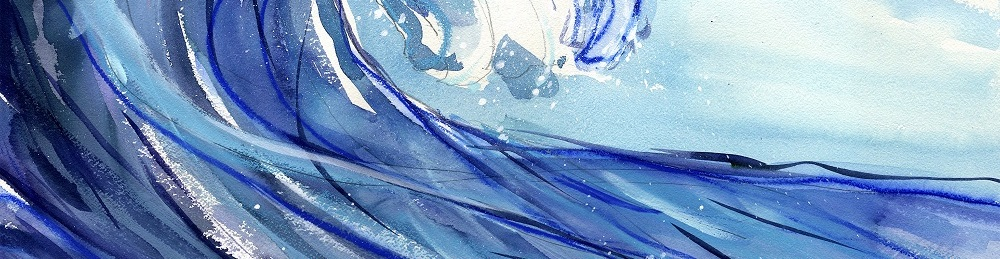
\includegraphics[width=.9\linewidth]{wave-simple}} 

\author{%
\begin{tabular}{c}
	Gabriel Peyr{\'e} \\ CNRS \& DMA \\
	 \'Ecole Normale Sup\'erieure \\
	 \url{gabriel.peyre@ens.fr}\\
	 \url{https://mathematical-tours.github.io}
\end{tabular}
}


\date{\today}

\begin{document}

\maketitle

% !TEX root = ../IntroImaging.tex

\chapter*{Presentation}


The four chapters of this text are independent and present gentle introductions to a few important mathematical foundations of data sciences:
\begin{itemize}
	\item Chapter~\ref{chap-shannon} presents Shannon theory of compression, and insists in particular on the entropy bound for coding of information.
	\item Chapter~\ref{chap-images} presents the basics of image processing, in particular some important processings (quantization, densoising, colors).
	\item Chapter~\ref{chap-sparsity} presents sampling theory, from Shannon classical sampling to compressed sensing. It also serves as a gentle introduction to the field of inverse problems regularization.
	\item Chapter~\ref{chap-ot} presents optimal transport and its applications to data sciences.
\end{itemize}
The exposition level for the first two chapters is elementary. The last chapter presents more advanced mathematical concepts and results. 


\tableofcontents
% !TEX root = ../FundationsDataScience.tex

\chapter{Shannon Theory}
\label{sec-shannon}

%
Shannon theory of information, published in 1948/1949, is made of three parts:
\begin{enumerate}
	\item Sampling: it studies condition under which sampling a continuous function to obtain a discrete vector is invertible. The discrete real values representing the signal are then typically quantized to a finite precision to obtain a set of symbols in a finite alphabet.  
	\item Source coding: it studies optimal ways to represent (code) such a set of symbols as a binary sequence. It leverages the statistical distributions to obtain the most possible compact code.  
	\item Channel coding (not studied here): it studies how to add some redundancy to the coded sequence in order to gain robustness to errors or attacks during transmission (flip of certain bits with some probability). It is often named ``error correcting codes theory''. 
\end{enumerate}
%
The main reference for this chapter is~\cite{mallat2008wavelet}.


%%%%%%%%%%%%%%%%%%%%%%%%%%%%%%%%%%%%%%%%%%%%%%%%%%%%%%%%%%%%%%%%%%%%
%%%%%%%%%%%%%%%%%%%%%%%%%%%%%%%%%%%%%%%%%%%%%%%%%%%%%%%%%%%%%%%%%%%%
%%%%%%%%%%%%%%%%%%%%%%%%%%%%%%%%%%%%%%%%%%%%%%%%%%%%%%%%%%%%%%%%%%%%
\section{Analog vs. Discrete Signals}

To develop numerical tools and analyze their performances, the mathematical modelling is usually done over a continuous setting (so-called ``analog signals''). 
%
Such continuous setting also aims at representing the signal in the physical world, which are inputs to sensors hardwares such as microphone, digital cameras or medical imaging devices. 
%
An analog signal is a 1-D function $f_0 \in \Ldeux([0,1])$ where $[0,1]$ denotes the domain of acquisition, which might for instance be time. An analog image is a 2D function $f_0 \in \Ldeux([0,1]^2)$ where the unit square $[0,1]^2$ is the image domain.

Although these notes are focussed on the processing of sounds and natural images, most of the methods extend to multi-dimensional datasets, which are higher dimensional mappings
\eq{
	f_0 : [0,1]^d \rightarrow [0,1]^s
}
where $d$ is the dimensionality of the input space ($d=1$ for sound and $d=2$ for images) whereas $s$ is the dimensionality of the feature space. For instance, gray scale images corresponds to $(d=2,s=1)$, 
videos to $(d=3, s=1)$, color images to $(d=2, s=3)$ where one has three channels $(R,G,B)$.
One can even consider multi-spectral images where $(d=2, s \gg 3)$ that is made of a large number of channels for different light wavelengths. Figures \ref{fig-examples-1} and \ref{fig-examples-2} show examples of such data.


\myfigure{
	\image{orthobases}{.35}{example-sound}
	\image{orthobases}{.28}{example-image}
	\image{orthobases}{.3}{example-video}
}{%
	Examples of sounds ($d=1$), image ($d=2$) and videos ($d=3$). %	
}{fig-examples-1}

\myfigure{
	\image{orthobases}{.4}{example-color}
	\image{orthobases}{.5}{example-multispectral}
}{%
	Example of color image $s=3$ and multispectral image ($s=32$). %	
}{fig-examples-2}


%%%%%%%%%%%%%%%%%%%%%%%%%%%%%%%%%%%%%%%%%%%
\subsection{Acquisition and Sampling}

Signal acquisition is a low dimensional projection of the continuous signal performed by some hardware device. This is for instance the case for a microphone that acquires 1D samples or a digital camera that acquires 2D pixel samples.
The sampling operation thus corresponds to mapping from the set of continuous functions to a discrete finite dimensional vector with $N$ entries.
\eq{
	f_0 \in \Ldeux([0,1]^d) \mapsto f \in \CC^N
}

\myfigure{
	\image{orthobases}{.4}{discretization-image}
	\image{orthobases}{.5}{discretization-sound}
}{%
	Image and sound discretization. %	
}{fig-discretization}

Figure \ref{fig-discretization} shows examples of discretized signals.

%%%%%%%%%%%%%%%%%%%%%%%%%%%%%%%%%%%%%%%%%%%
\subsection{Linear Translation Invariant Sampler}

A translation invariant sampler performs the acquisition as an inner product between the continuous signal and a constant impulse response $h$ translated at the sample location
\eql{\label{eq-linear-sampling}
	f_n = \int_{-S/2}^{S/2} f_0(x) h(n/N - x) \d x= f_0 \star h(n/N).
}
The precise shape of $h(x)$ depends on the sampling device, and is usually a smooth low pass function that is maximal around $x=0$. The size $S$ of the sampler determines the precision of the sampling device, and is usually of the order of $1/N$ to avoid blurring (if $S$ is too large) or aliasing (if $S$ is too small).

Section \ref{sec-sampling} details how to reverse the sampling operation in the case where the function is smooth.


%%%%%%%%%%%%%%%%%%%%%%%%%%%%%%%%%%%%%%%%%%%%%%%%%%%%%%%%%%%%%%%%%%%%
%%%%%%%%%%%%%%%%%%%%%%%%%%%%%%%%%%%%%%%%%%%%%%%%%%%%%%%%%%%%%%%%%%%%
%%%%%%%%%%%%%%%%%%%%%%%%%%%%%%%%%%%%%%%%%%%%%%%%%%%%%%%%%%%%%%%%%%%%
\section{Shannon Sampling Theorem}
\label{subsec-sampling}

%%%
\paragraph{Reminders about Fourier transform.}

For $f \in L^1(\RR)$, its Fourier transform is defined as
\eql{\label{eq-fourier-transform}
	\foralls \om \in \RR, \quad
	\hat f(\om) \eqdef \int_\RR f(x) e^{-\imath x \om} \d x.
}
One has $\norm{\hat f}^2 = (2\pi)^{-1} \norm{f}^2$, so that $f \mapsto \hat f$ can be extended by continuity to $L^2(\RR)$, which corresponds to computing $\hat f$ as a limit when $T \rightarrow +\infty$ of $\int_{-T}^T f(x) e^{-\imath x \om} \d x$.
%
When $\hat f \in L^1(\RR)$, one can invert the Fourier transform so that
\eql{\label{eq-i-ft}
	f(x) = \frac{1}{2\pi} \int_\RR \hat f(\om) e^{\imath x \om} \d \om, 
}
which shows in particular that $f$ is continuous with vanishing limits at $\pm\infty$. 

The Fourier transform $\Ff : f \mapsto \hat f$ exchanges regularity and decay. For instance, if $f \in C^p(\RR)$ with an integrable Fourier transform, then $\Ff(f^{(p)})(\om) = (\imath \om)^{p} \hat f(\om)$ so that $|\hat f(\om)|=O(1/|\om|^p)$. 
%
Conversely, 
\eql{\label{eq-fourier-regul}
	\int_\RR (1+|\om|)^{p} |\hat f(\om)| \d \om<+\infty
	\qarrq f \in C^p(\RR).
}
For instance, if $\hat f(\om)=O(1/|\om|^{p+2})$, one obtains that $f \in C^p(\RR)$. 

%%%
\paragraph{Reminders about Fourier series.}

We denote $\TT=\RR/2\pi\ZZ$ the torus.
%
A function $f \in L^2(\TT)$ is $2\pi$-periodic, and can be viewed as a function $f \in L^2([0,2\pi])$ (beware that this means that the boundary points are glued together), and its Fourier coefficients are
\eq{
	\foralls n \in \ZZ, \quad 
	\hat f_n \eqdef \frac{1}{2\pi}\int_0^{2\pi} f(x) e^{-\imath x n} \d x.
}
This formula is equivalent to the computation of an inner-product $\hat f_n = \dotp{f}{e_n}$ for the inner-product $\dotp{f}{g} \eqdef \frac{1}{2\pi} \int_\TT f(x) \bar g(x) \d x$. 
%
For this inner product, $(e_n)_n$ is orthonormal and is actually an Hilbert basis, meaning that one reconstructs with the following converging series 
\eql{\label{eq-fourier-series}
	f = \sum_{n \in \ZZ} \dotp{f}{e_n} e_n
}
which means $\norm{f-\sum_{n=-N}^N \dotp{f}{e_n} e_n}_{L^2(\TT)} \rightarrow 0$ for $N \rightarrow +\infty$.
%
The pointwise convergence of~\eqref{eq-fourier-series} at some $x \in \TT$ is ensured if for instance $f$ is differentiable. The series is normally convergent (and hence uniform) if for instance $f$ if of class $C^2$ on $\TT$ sin ce in this case, $\hat f_n = O(1/n^2)$. 
%
If there is a step discontinuities, then there is Gibbs oscillations preventing uniform convergence, but the series still converges to the half of the left and right limit.


%%%
\paragraph{Poisson formula.}

The poisson formula connects the Fourier transform and the Fourier series to sampling and periodization operators.
%
For some function $h(t)$ defined on $\RR$ (typically the goal is to apply this to $h=\hat f$), its periodization reads
\eql{\label{eq-periodizing}
	h_P(t) \eqdef \sum_n h(t-2\pi n).
} 
This formula makes sense if $h \in L^1(\RR)$, and in this case $\norm{h_P}_{L^1(\TT)} \leq \norm{h}_{L^1(\RR)}$ (and there is equality for positive functions). 
%
The Poisson formula, stated in Proposition~\ref{prop-poisson} bellow, corresponds to proving that the following diagram
\eq{
	\begin{array}{rcccl}
						& f(x)  &  \overset{\Ff}{\longrightarrow} &  \hat f(\om) &\\
		\text{sampling}& \downarrow & & \downarrow &\text{periodization} \\
						& (f(n))_n  &  \overset{\text{Fourier serie}}{\longrightarrow} &  \sum_n f(n) e^{-\imath \om n} &\\
	\end{array}
}
is actually commutative.

\begin{prop}[Poisson formula]\label{prop-poisson}
Assume that $\hat f$ has compact support and that $|f(x)| \leq C(1+|x|)^{-3}$ for some $C$. Then one has 
\eql{\label{eq-poisson-formula}
	\foralls \om \in \RR, \quad
	\sum_n f(n) e^{-\imath \om n} = \hat f_P(\om).
}
\end{prop}
\begin{proof}
	Since $\hat f$ is compactly supported, $\hat f_P$ is well defined (it involves only a finite sum) and since $f$ has fast decay, using~\eqref{eq-fourier-regul}, $(\hat f)_P$ is $C^1$. It is thus the sum of its Fourier series
	\eql{\label{eq-poisson-formula}
		(\hat f)_P(\om) = \sum_k c_k e^{\imath k \om},
	} 
	where
	\begin{align*}
		c_k = \frac{1}{2\pi} \int_0^{2\pi} (\hat f)_P(\om) e^{-\imath k \om} \d \om = 
		\frac{1}{2\pi} \int_0^{2\pi} \sum_n \hat f(\om-2\pi n) e^{-\imath k \om}  \d \om .
	\end{align*}
	One has 
	\eq{
		\int_0^{2\pi} \sum_n |\hat f(\om-2\pi n) e^{-\imath k \om}|  \d \om = \int_\RR |\hat f| 
	}
	which is bounded because $\hat f \in L^1(\RR)$ (it has a compact support and is $C^1$), so one can exchange the sum and integral
	\eq{
		c_k = \sum_n \frac{1}{2\pi} \int_0^{2\pi} \hat f(\om-2\pi  n) e^{-\imath k \om}  \d \om
		= \frac{1}{2\pi} \int_{\RR} \hat f(\om) e^{-\imath k \om}  \d \om
		= f(-k)
	}
	where we used the inverse Fourier transform formula~\eqref{eq-i-ft}, which is legit because $\hat f \in L^1(\RR)$.
\end{proof}

%%%
\paragraph{Shannon theorem.}

Shannon sampling theorem state a sufficient condition ensuring that the sampling operator $f \mapsto (f(ns))_n$ is invertible for some sampling step size $s>0$. 
%
It require that $\supp(\hat f) \subset [-\pi/s,\pi/s]$, which, thanks to formula~\eqref{eq-i-ft}, implies that $\hat f$ is $C^\infty$ (in fact it is even analytic). 
%
This theorem was first proved by Wittaker in 1915. It was re-proved and put in perspective in electrical engineering by Nyquist in 1928. It became famous after the paper of Shannon in 1949, which put forward its importance in numerical communications.
%
Figure~\ref{fig-sampling-aliasing} give some insight on how the proof works (left) and more importantly, on what happens when the compact support hypothesis fails (in which case aliasing occurs, see also Figure~\ref{fig-aliasing}). 

\myfigure{
	\image{1-shannon}{.8}{sampling-aliasing}
}{%
	Schematic view for the proof of Theorem~\ref{thm-shannon-sampling}. %	
}{fig-sampling-aliasing}





\begin{thm} \label{thm-shannon-sampling}
	If $|f(x)| \leq C(1+|x|)^{-3}$ for some $C$ and $\supp(\hat f) \subset [-\pi/s,\pi/s]$, then one has
	\eql{\label{eq-shannong-interp}
		\foralls x \in \RR, \quad 
		f(x) = \sum_n f(n s) \sinc(x/s-n) \qwhereq
		\sinc(u) = \frac{\sin(\pi u)}{\pi u}
	}
	with uniform convergence.
\end{thm}

\begin{proof} 
	The change of variable $g \eqdef f(s \cdot)$ results in $\hat g=1/s \hat f(\cdot/s)$, indeed, denoting $z=s x$
	\eq{
		\hat g(\om) = \int f(s x) e^{-\imath \om x} \d x = \frac{1}{s} \int f(z) e^{-\imath (\om/s) z} \d z = \hat f(\om/s)/s, 
	} 
	so that we can restrict our attention to $s=1$.
	%
	The compact support hypothesis implies $\hat f(\om) = 1_{[-\pi,\pi]}(\om) \hat f_P(\om)$.  
	Combining the inversion formula~\eqref{eq-i-ft} with Poisson formula~\eqref{eq-poisson-formula}
	\eq{
		f(x) = \frac{1}{2\pi} \int_{-\pi}^\pi \hat f_P(\om) e^{\imath \om x} \d \om
		= \frac{1}{2\pi} \int_{-\pi}^\pi \sum_n f(n) e^{\imath \om (x-n)} \d \om.
	} 
	Since $f$ has fast decay, $\int_{-\pi}^\pi \sum_n |f(n) e^{\imath \om (x-n)}| \d \om = \sum_n |f(n)| < +\infty$, so that one can exchange summation and integration and obtain
	\eq{
		f(x) = \sum_n f(n)  \frac{1}{2\pi} \int_{-\pi}^\pi e^{\imath \om (x-n)} \d \om = \sum_n f(n) \sinc(x-n).
	}
\end{proof}

\wrapf{1-shannon/sinc}{sinc kernel}
One issue with this reconstruction formula is that it uses a slowly decaying and very oscillating $\sinc$ kernels. In practice, one rarely uses such a kernel for interpolation, and one prefers smoother and more localized kernel. If $\supp(\hat f) \subset [-\pi/s',\pi/s']$ with $s'>s$ (i.e. have a more compact spectrum), one can re-do the proof of the theorem, and one gains some degree of freedom to design the reconstruction kernel, which now can be chosen smoother in Fourier and hence have exponential decay in time. 

%
Spline interpolation are defined by considering $\phi_0=1_{[-1/2,1/2]}$ and $\phi_k = \phi_{k-1} \star \phi_0$ which is a piecewise polynomial of degree $k$ and has bounded derivative of order $k$ (and is of class $C^{k-1}$) with compact support on $[-(k+1)/2,(k+1)/2]$. The reconstruction formula reads $f \approx \tilde f \eqdef \sum_n a_n \phi(\cdot-n)$ where $(a_n)_n$ is computed from the $(f(n))_n$ by solving a linear system (associated to the interpolation property $\tilde f(n)=f(n)$). It is only in the cases $k \in \{0,1\}$ (piecewise constant and affine interpolations) that one has $a_n=f(n)$.
%
In practice, one typically use the cubic spline interpolation, which corresponds to $k=3$.

\texttt{Associated code: test\_sampling.m}

\myfigure{
	\image{1-shannon}{.6}{spline}
}{%
	Cardinal splines as bases functions for interpolation. %	
}{fig-aliasing}



This theorem also explains what happens if $\hat f$ is not supported in $[-\pi/s,\pi/s]$. This leads to aliasing, and high frequency outside this interval leads to low frequency artifacts often referred to as ``aliasing''. If the input signal is not bandlimitted, it is thus very important to pre-filter it (smooth it) before sampling to avoid this phenomena (of course this kills the high frequencies, which are lost), see Figure~\ref{fig-aliasing}. 

\myfigure{
	\image{1-shannon}{.6}{aliasing}
}{%
	Aliasing in the simple case of a sine wave (beware however that this function does not have compact support). %	
}{fig-aliasing}

%%%
\paragraph{Quantization.}

Once the signal have been sampled to obtain a discrete vector, in order to store it and transmit it, it is necessary to quantize the value to some finite precision. 
% 
Section~\ref{sec-transform-coding} presents transform coding, which is an efficient family of compression schemes which operate the quantization over some transformed domain (which correspond to applying a linear transform, usually orthogonal, to the sampled values). This is useful to enhance the performance of the source coding scheme. It is however common to operate directly the quantization over the sampled value. 

Considering for instance a step size $s=1/N$, one samples $(u_n \eqdef f(n/N))_{n=1}^{N} \in \RR^N$ to obtain a finite dimensional data vector of length $N$. Note that dealing with finite data corresponds to restricting the function $f$ to some compact domain (here $[0,1]$) and is contradictory with Shannon sampling theorem, since a function $f$ cannot have a compact support in both space and frequency (so perfect reconstruction never holds when using finite storage).

\wrapf{1-shannon/quantizer}{}

Choosing a quantization step $T$, quantization $v_n = Q_T(u_n) \in \ZZ$ rounds to the nearest multiple of $T$, i.e. 
\eq{
	v = Q_T(u) \quad\Leftrightarrow\quad
	v-\frac{1}{2} \leq u/T < v+\frac{1}{2},
}
see Fig.~\ref{fig-quantizer}. De-quantization is needed to restore a signal, and the best reconstruction (in average or in worse case) is defined by setting $D_T(v) \eqdef T v$. Quantizing and then de-quantizing introduce an error bounded by $T/2$, since $|D_T(Q_T(u))-u| \leq T/2$. 
%
Up to machine precision, quantization is the only source of error (often called ``lossy compression'') in Shannon's standard pipeline.


\myfigure{
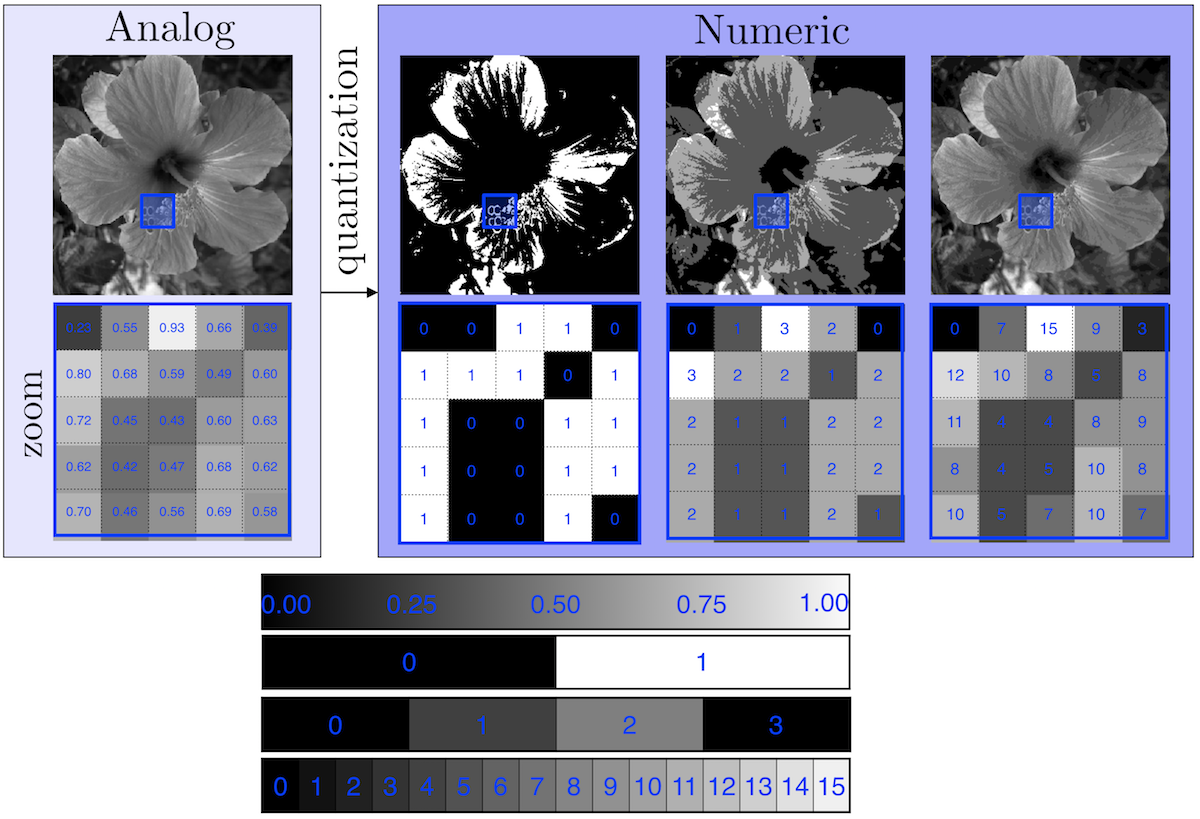
\includegraphics[width=.8\linewidth]{1-shannon/quantize/quantization}
%\tabquatre{
%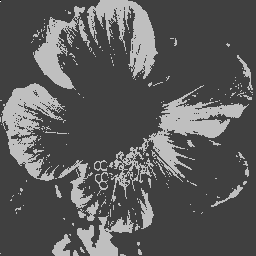
\includegraphics[width=.2\linewidth]{1-shannon/quantize/quantize-2}&
%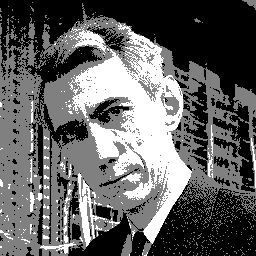
\includegraphics[width=.2\linewidth]{1-shannon/quantize/quantize-3}&
%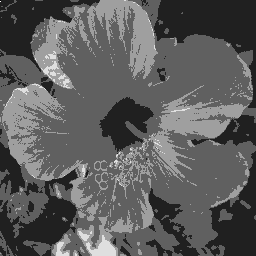
\includegraphics[width=.2\linewidth]{1-shannon/quantize/quantize-4}&
%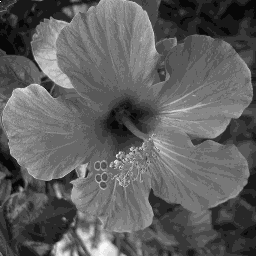
\includegraphics[width=.2\linewidth]{1-shannon/quantize/quantize-16}\\
%$2$ graylevels &
%$3$ graylevels &
%$4$ graylevels &
%$16$ graylevels 
%}
}{Quantizing an image using a decaying $T=1/K$ where $K \in \{2,3,4,16\}$ is the number of graylevels and the original image is normalized so that $0 \leq f_0 < 1$. 
}{fig-section3-quantize}

%%%%%%%%%%%%%%%%%%%%%%%%%%%%%%%%%%%%%%%%%%%%%%%%%%%%%%%%%%%%%%%%%%%%
\section{Shannon Source Coding Theorem}
\label{sec-shannon-source}

\newcommand{\Symb}{s}

%%%
\paragraph{Uniform coding.}

We consider an alphabet $(\Symb_1,\ldots,\Symb_K)$ of $K$ symbols. For instance, if one samples and quantize a bounded signal $0 \leq f_0 < 1$ using a step size $1/K$, then one can consider $\Symb_k=k$ to be integer symbols. For text, these symbols include the letter plus extra punctuation symbols and blank. 
%
It is of course possible to code a sequence of such symbols using a uniform code (e.g. using the base 2 expansion) with $\lceil \log_2(K) \rceil$ bit per symbols.
For instance if $K=4$ and the symbols are $\{0,1,2,3\}$, then the code words are $(c_0=00,c_1=01,c_2=10,c_3=11)$. 

This uniform coding strategy is however extremely inefficient if the symbols are not uniformly distributed (i.e. if some symbols are more frequent than other, which is likely to be the case). We aim at designing better codes.

%%%
\paragraph{Prefix coding.}
 

A code $c_k=c(\Symb_k)$ associate to each symbol $\Symb_k$ a code word $c_k \in \{0,1\}^\NN$ with a varying length $|c_k| \in \NN^*$. 
%
A prefix code $c_k=c(\Symb_k)$ is such that no word $c_k$ is the beginning of another word $c_k'$. This is equivalent to be able to embed the $(c_k)_k$ as leaves of a binary tree $T$, with the code being output of a traversal from root to leaves (with a convention that going to a left (resp. right) child output a 0 (resp. a 1). 
%
We denote $c=\text{Leaves}(T)$ such prefix property. 


\myfigure{
\image{1-shannon}{.35}{tree/prefix-coding}
\qquad
\image{1-shannon}{.35}{tree/tree-example}
}{%
Left: complete tree of all codes of length 3; right: example of prefix code.
}{fig-tree-prefix}

This tree-based representation is useful to decode a binary stream by simply performing tree traversal. One follows the tree, from top to bottom, and outputs a symbol each time a leaf is reached (and then re-start at the top). 

The following fundamental lemma describes the set of prefix codes using an inequality.

\begin{lem}[Kraft inequality]\label{lem-kraft}
	(i) For a code $c$, if there exists a tree $T$ such that $c=\text{Leaves}(T)$ then
	\eql{\label{eq-kraft-ineg}
		\sum_k 2^{-|c_k|} \leq 1.
	}
	(ii) Conversely, if $(\ell_k)_k$ are such that
	\eql{\label{eq-kraft-ineg-2}
		\sum_k 2^{-\ell_k} \leq 1
	}
	then there exists a code $c=\text{Leaves}(T)$ such that $|c_k|=\ell_k$.
\end{lem} 

\begin{proof}
	$\Rightarrow$ We suppose $c=\text{Leaves}(T)$. We denote $m=\max_k |c_k|$ and consider the full binary tree.
	%
	Bellow each $c_k$, one has a sub-tree of height $m-|c_k|$, see Figure~\ref{fig-fourier-wav}, left. This sub-tree has $2^{m-|c_k|}$ leaves. Since all these sub-trees do not overlap, the total number of leaf do not exceed the total number of leaves $2^m$ of the full binary tree, hence
	\eq{
		\sum_k 2^{m-|c_k|} \leq 2^m, 
	}
	hence~\eqref{eq-kraft-ineg}. 
	
	\myfigure{
	\image{1-shannon}{.35}{kraft-ineq-1}\quad
	\image{1-shannon}{.45}{kraft-ineq-2}
}{%
	Left: full binary tree obtained by completing the tree associated to the code $(c_1=0, c_2=10, c_3=110, c_4=111)$. 
	%
	Right: packing sub-trees associated to code length to form the left part of the full tree. %	
}{fig-fourier-wav}

	
	$\Leftarrow$ Conversely, we assume~\eqref{eq-kraft-ineg} holds. Without loss of generality, we assume that $|c_1| \geq \ldots \geq |c_K|$. We start by putting a sub-tree of height $2^{m-|c_1|}$. Since the second tree is smaller, one can put it immediately aside, and continue this way, see Figure~\ref{fig-fourier-wav}, right. Since  $\sum_k 2^{m-|c_k|} \leq 2^m$, this ensure that we can stack side-by-side all these sub-tree, and this defines a proper sub-tree of the full binary tree. 
\end{proof}


%%
\paragraph{Probabilistic modeling.}

We aim at designing the most possible compact code $c_k$. 
%
We assume at our disposal some probability distribution over this alphabet, which is just an histogram $p=(p_1,\ldots,p_K) \in \RR_+^K$ in the simplex, i.e. $\sum_k p_k=1$. 
%
In practice, this probability is usually the empirical probability of appearance of the symbols $x_k$ in the data to be coded. 

\wrapf{1-shannon/entropie/entropie-fonction}{}

The entropy of such an histogram is 
\eq{
	H(p) \eqdef -\sum_k p_k \log_2(p_k)
}
with the convention $0\log_2(0)=0$. 

Denoting $h(u)=-u \log(u)$, $h'(u)=-\log(u)-1$, $h''(u)=-1/u<0$ so that $H$ is strictly concave. The definition of the entropy extends to continuous density $f(x)$ for $x$ on some measure space with reference measure $\d x$ (e.g. Lebesgue on $\RR^d$) by setting $H(f)=-\int f(x) \log(f(x)) \d x$. 

\myfigure{
\tabquatre{
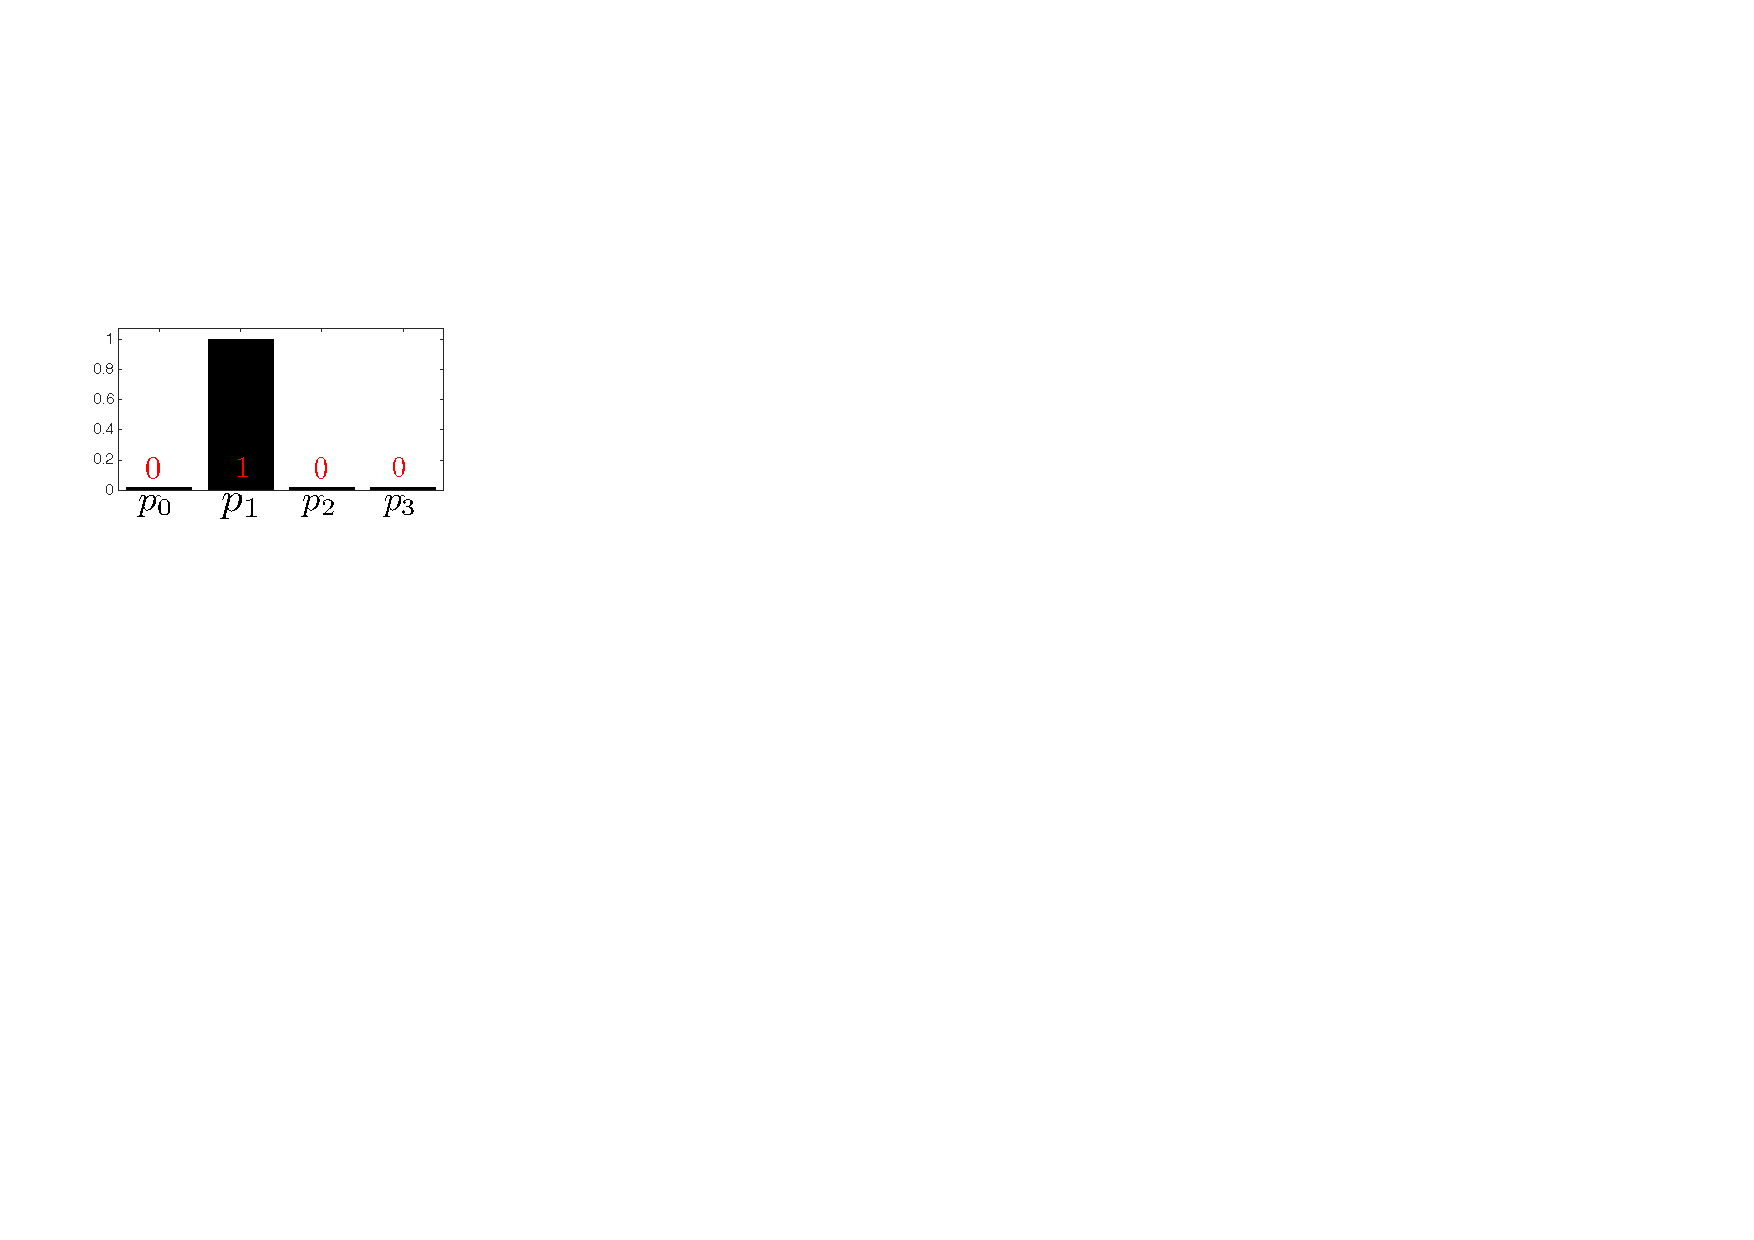
\includegraphics[width=.25\linewidth]{1-shannon/entropie/histo-1}&
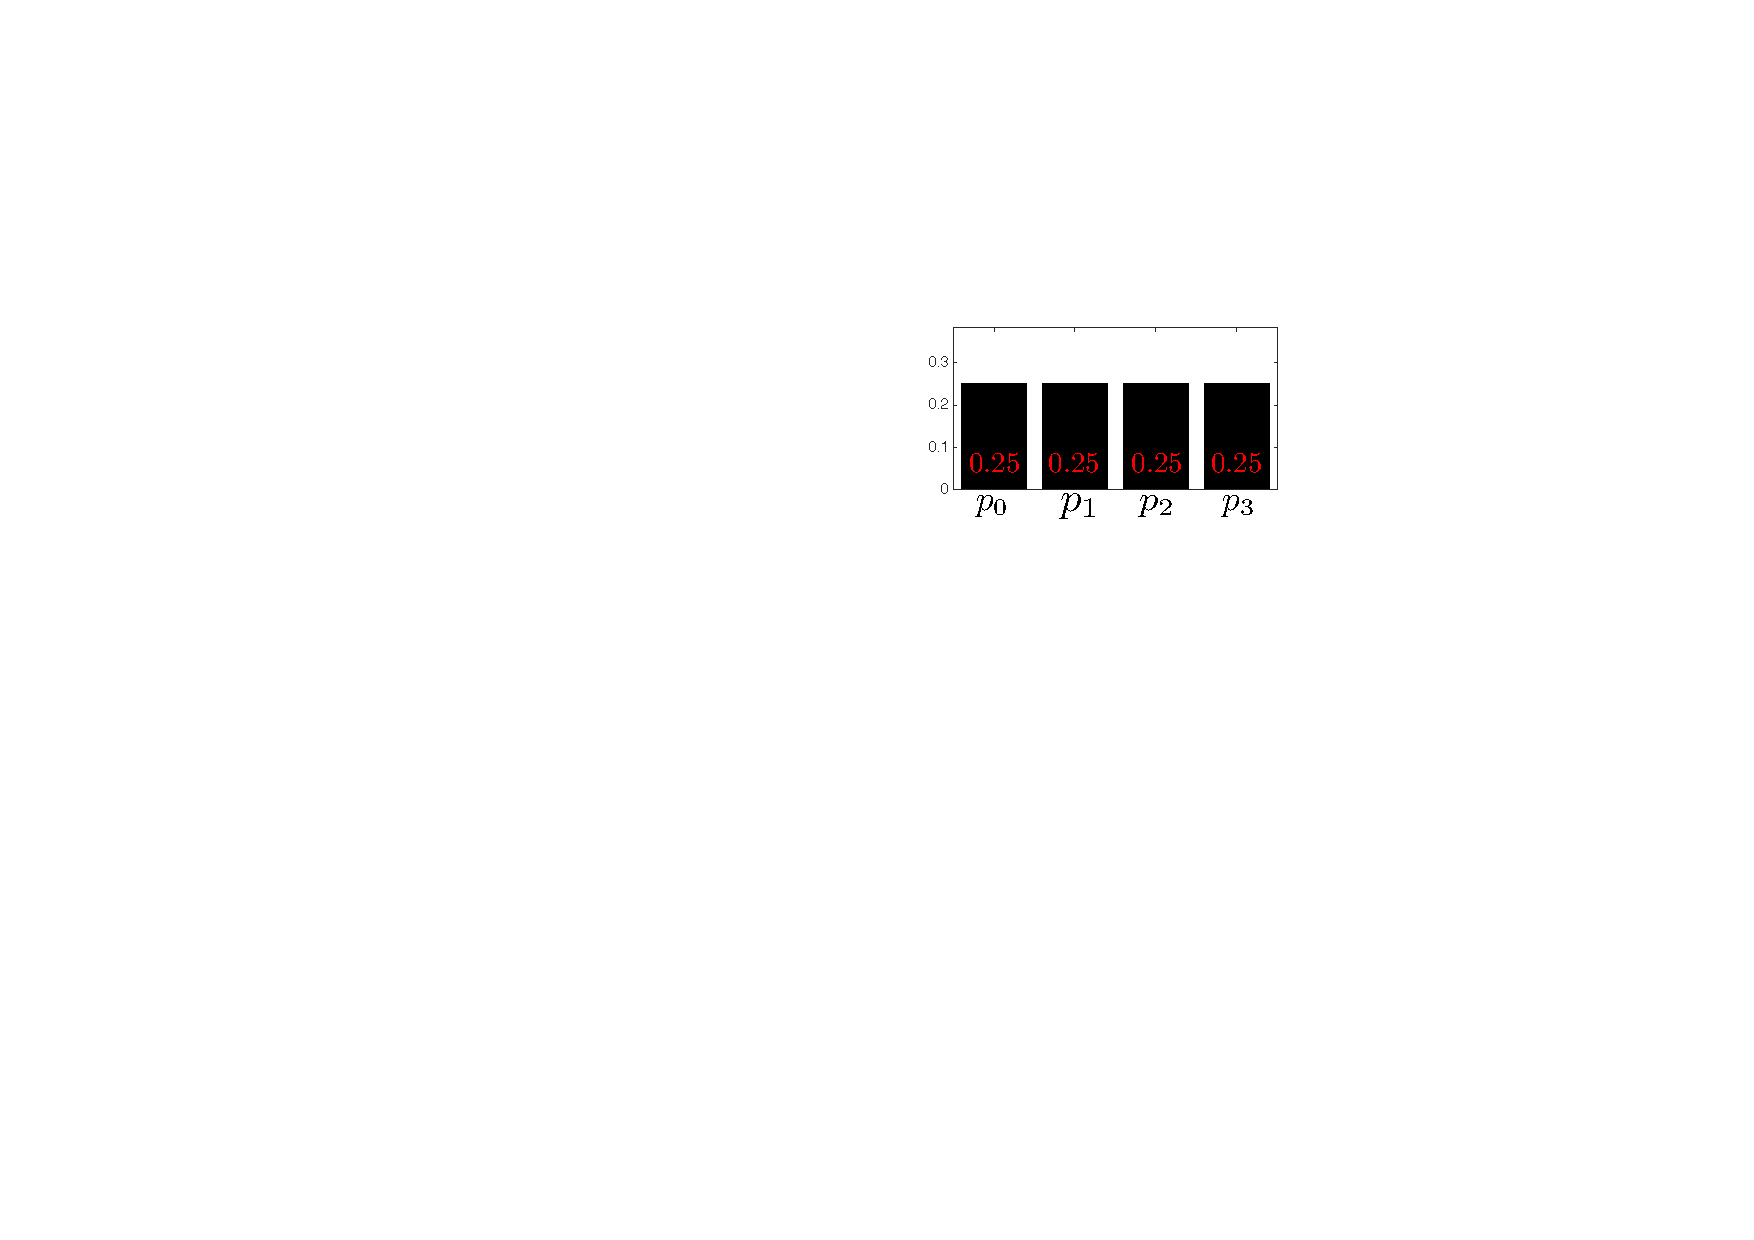
\includegraphics[width=.25\linewidth]{1-shannon/entropie/histo-3}&
\includegraphics[width=.25\linewidth]{1-shannon/entropie/histo-sub}\\
$H(p)=0$ & $H(p)=\log_2(2)=1$ &  $H(p) = 1.62$
}
}{Three examples of probability distributions with corresponding entropies.}{fig-histo-entropy}


\myfigure{
	\image{1-shannon}{.35}{entropy-extrema}
}{%
	Linked extra for the entropy. %	
}{fig-entropy-extrema}



\begin{lem} One has
\eq{
	0 \leq H(p) \leq \log_2(K).
}
\end{lem}


\begin{proof}
	We consider the following constrained optimization problem
	\eq{
		\min_p \enscond{ f(p) }{ g(p) = \sum_k p_k =1 }
	}
	where $f=-H$, see Fig.~\ref{fig-entropy-extrema}. According to the linked extrema theorem, at an optimum $p^\star$, $\nabla f(p^\star)=\la \nabla g(p^\star)$ for some $\la \in \RR$, so that here $\log(p_k^\star)+1 = \la$, i.e. $p_k^\star=c$ is constant, and since 
	$\sum_k p_k^\star=1$, 	
	one has $p_k^*=1/K$ and thus $H(p)=\log_2(K)$.
\end{proof}


%%
\paragraph{Shannon theorem.}

%
Assuming that $(p_k)_k$ is the empirical probability of appearance of the symbols $x_k$ in the data to be coded, the average symbol length associated to some code $c$ is 
\eq{
	L(c) \eqdef \sum_k p_k |c_k|. 
}
The goal is to design the best possible $c$ so that $L(c)$ is as small as possible.
%
Shannon theorem of entropic coding, proved bellow, give both lower and upper bound for this question. 

\begin{thm}
	(i) If $c=\text{Leaves}(T)$ for some tree $T$, then 
	\eq{
		L(c) \geq H(p).
	}
	(ii) Conversely, there exists a code $c$ with $c=\text{Leaves}(T)$ such that 
	\eq{
		L(c) \leq H(p)+1.
	}
\end{thm} 

\begin{proof}
	First, we consider the following optimization problem
	\eql{\label{eq-proof-shannon}
		\umin{ \ell = (\ell_k)_k } \enscond{ f(\ell) \eqdef \sum_k \ell_k p_k }{ g(\ell) \eqdef  \sum_k 2^{-\ell_k} \leq 1 }.
	}
	We fist show that at an optimal $\ell^\star$, the constraint is saturated, i.g. $g(\ell^\star)=1$. Indeed, if $g(\ell^\star)=2^{-u} < 1$, with $u>0$, we define $\ell_k' \eqdef \ell_k^\star-u$, which satisfies $g(\ell') = 1$ and also $f(\ell')=\sum_k (\ell_k-u) p_k < f(\ell^\star)$, which is a contradiction.
	So we can restrict in~\eqref{eq-proof-shannon} the constraint to $g(\ell)=1$ and apply the linked extrema theorem, which shows that necessarily, there exists $\la \in \RR$ with $\nabla f(\ell^\star)=\nabla g(\ell^\star)$, i.e.  $(p_k)_k = -\la \ln(2) (2^{-\ell_k^\star})_k$. Since 
	\eq{
		1 = \sum_k p_k = -\la \ln(2) \sum_k 2^{-\ell_k} = - \la \ln(2) 
	}
	we deduce that $\ell^\star_k = -\log(p_k)$. 
	
	(i) If $c=\text{Leave}(T)$, the by Kraft inequality~\eqref{eq-kraft-ineg}, necessarily $\ell_k=|c_k|$ satisfy the constraints of~\eqref{eq-proof-shannon}, and thus $H(p) = f(\ell^\star) \leq f(\ell) = L(\ell)$.
	
	(ii) We define $\ell_k \eqdef \lceil -\log_2(p_k) \rceil \in \NN^*$. Then $\sum_k 2^{-\ell_k} \leq \sum_k 2^{\log_2(p_k)} = 1$, so that these lengths satisfy~\eqref{eq-kraft-ineg-2}. Thanks to Proposition~\ref{lem-kraft} (ii), there thus exists a prefix code $c$ with $|c_k|=\lceil -\log_2(p_k) \rceil$. Furthermore
	\eq{
		L(c) = \sum_k p_k \lceil -\log_2(p_k) \rceil \leq \sum_k p_k ( -\log_2(p_k) +1) = H(p)+1.
	}
\end{proof}

Note that this proof is constructing, i.e. it gives an algorithm that construct an almost optimal $c$, and this code is often called the Shannon-Fano code. It is usually a good code, although it is not necessarily the optimal code with the smallest $L(c)$. Such an optimal code can easily be computed in almost linear time (only sorting of the probability is needed, so it is $K(\log(K))$) by Huffman's dynamic programming algorithm (invented in 1952). The proof of correctness of this algorithm is however a bit tedious. Figure~\ref{fig-huff-code} shows an example of application of this algorithm.


\texttt{Associated code: coding/test\_text.m}

In practice, such an entropic coding, although optimal, is not very efficient when one of the symbol has a large probability $p_k$. This is because then $2^{-p_k} \ll 1$ but one cannot allocate a fractional number of bit. This is why $L(c)$ can be as large as $H(p)+1$. A simple workaround is to artificially increase the size of the alphabet from $K$ to $K^r$ by grouping together sets of $r$ consecutive symbols, and thus reducing the gap to $H(p)+1/r$. Constructing the code and coding however becomes very slow for large $r$. The standard way to achieve this without explicitly doing the grouping is by using arithmetic coding, invented in 1976, which using interval arithmetic to allocate fractional number of bits and leveraging the fact that one usually code large sequence, thus approaching to arbitrary precision Shannon bound $H(p)$ as the length of the data increases.


\myfigure{
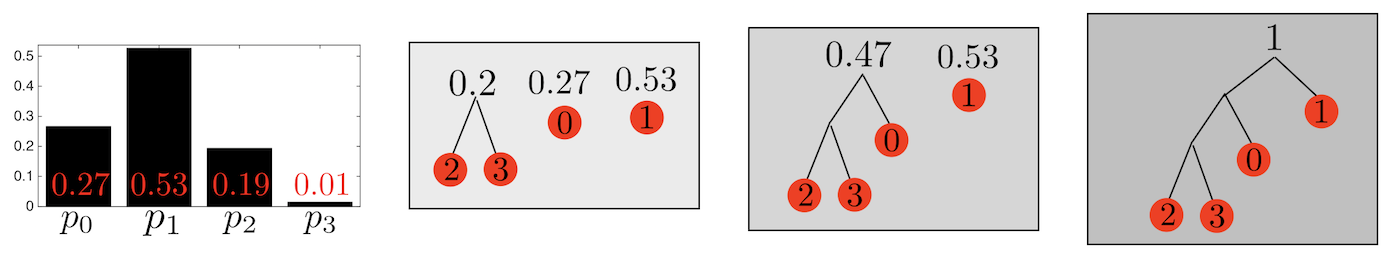
\includegraphics[width=.8\linewidth]{1-shannon/huff-code}
}{Huffman coding algorithm in action.}{fig-huff-code}

Note that while we give some statistical and probabilistic interpretation of entropy (measure of uncertainty) and of Shannon theorem, this theory is fully deterministic and give a bound for the actual length $N L(c)$ of coding some sequence of length $N$ if the probability $p$ are the empirical probability of the sequence.

If one choose a different probability $q$ and use it to code the sequence, one necessarily obtain a worse average coding length, and this is reflected by the positivity of the so-called relative entropy (beware that it is a convex function while the entropy is concave), which is often called the Kulback-Leibler divergence
\eq{
	\text{KL}(p|q) = -\sum_k p_k \log q_k - H(p)   = \sum_k p_k \log \frac{p_k}{q_k} \geq 0.
}
This KL divergence is similar to a distance in the sense that $\text{KL}(p|q)=0$ if and only if $p=q$ (note however that KL is not symmetric and does not satisfies the triangular inequality). It also has the remarkable property that it is jointly convex in $(p,q)$. It is of paramount importance to compare probability distributions and measures, and form the basis of the fields of information theory and information geometry. 


%%
\paragraph{Doing better.}

One can wonder if it is possible to go bellow the entropy bound. By the virtue of Shannon theorem, it is not possible if only can only code in sequential order the symbols themselves. From a statistical perspective, it is as if the symbols where considered to be independent. If there is some redundancy in the sequence of symbol (for instance if they are discretization of a smooth function, so that to consecutive symbols are likely to be equal), it is possible to re-transform (in a bijective way) the sequence to make them ``more independent''. A simple illustration of this idea is given in Figure~\ref{fig-codage-differences}, where one computes successive difference of a 1D sequence of symbols (beware to also retain the initial symbol to be able to do the decoding.

\myfigure{
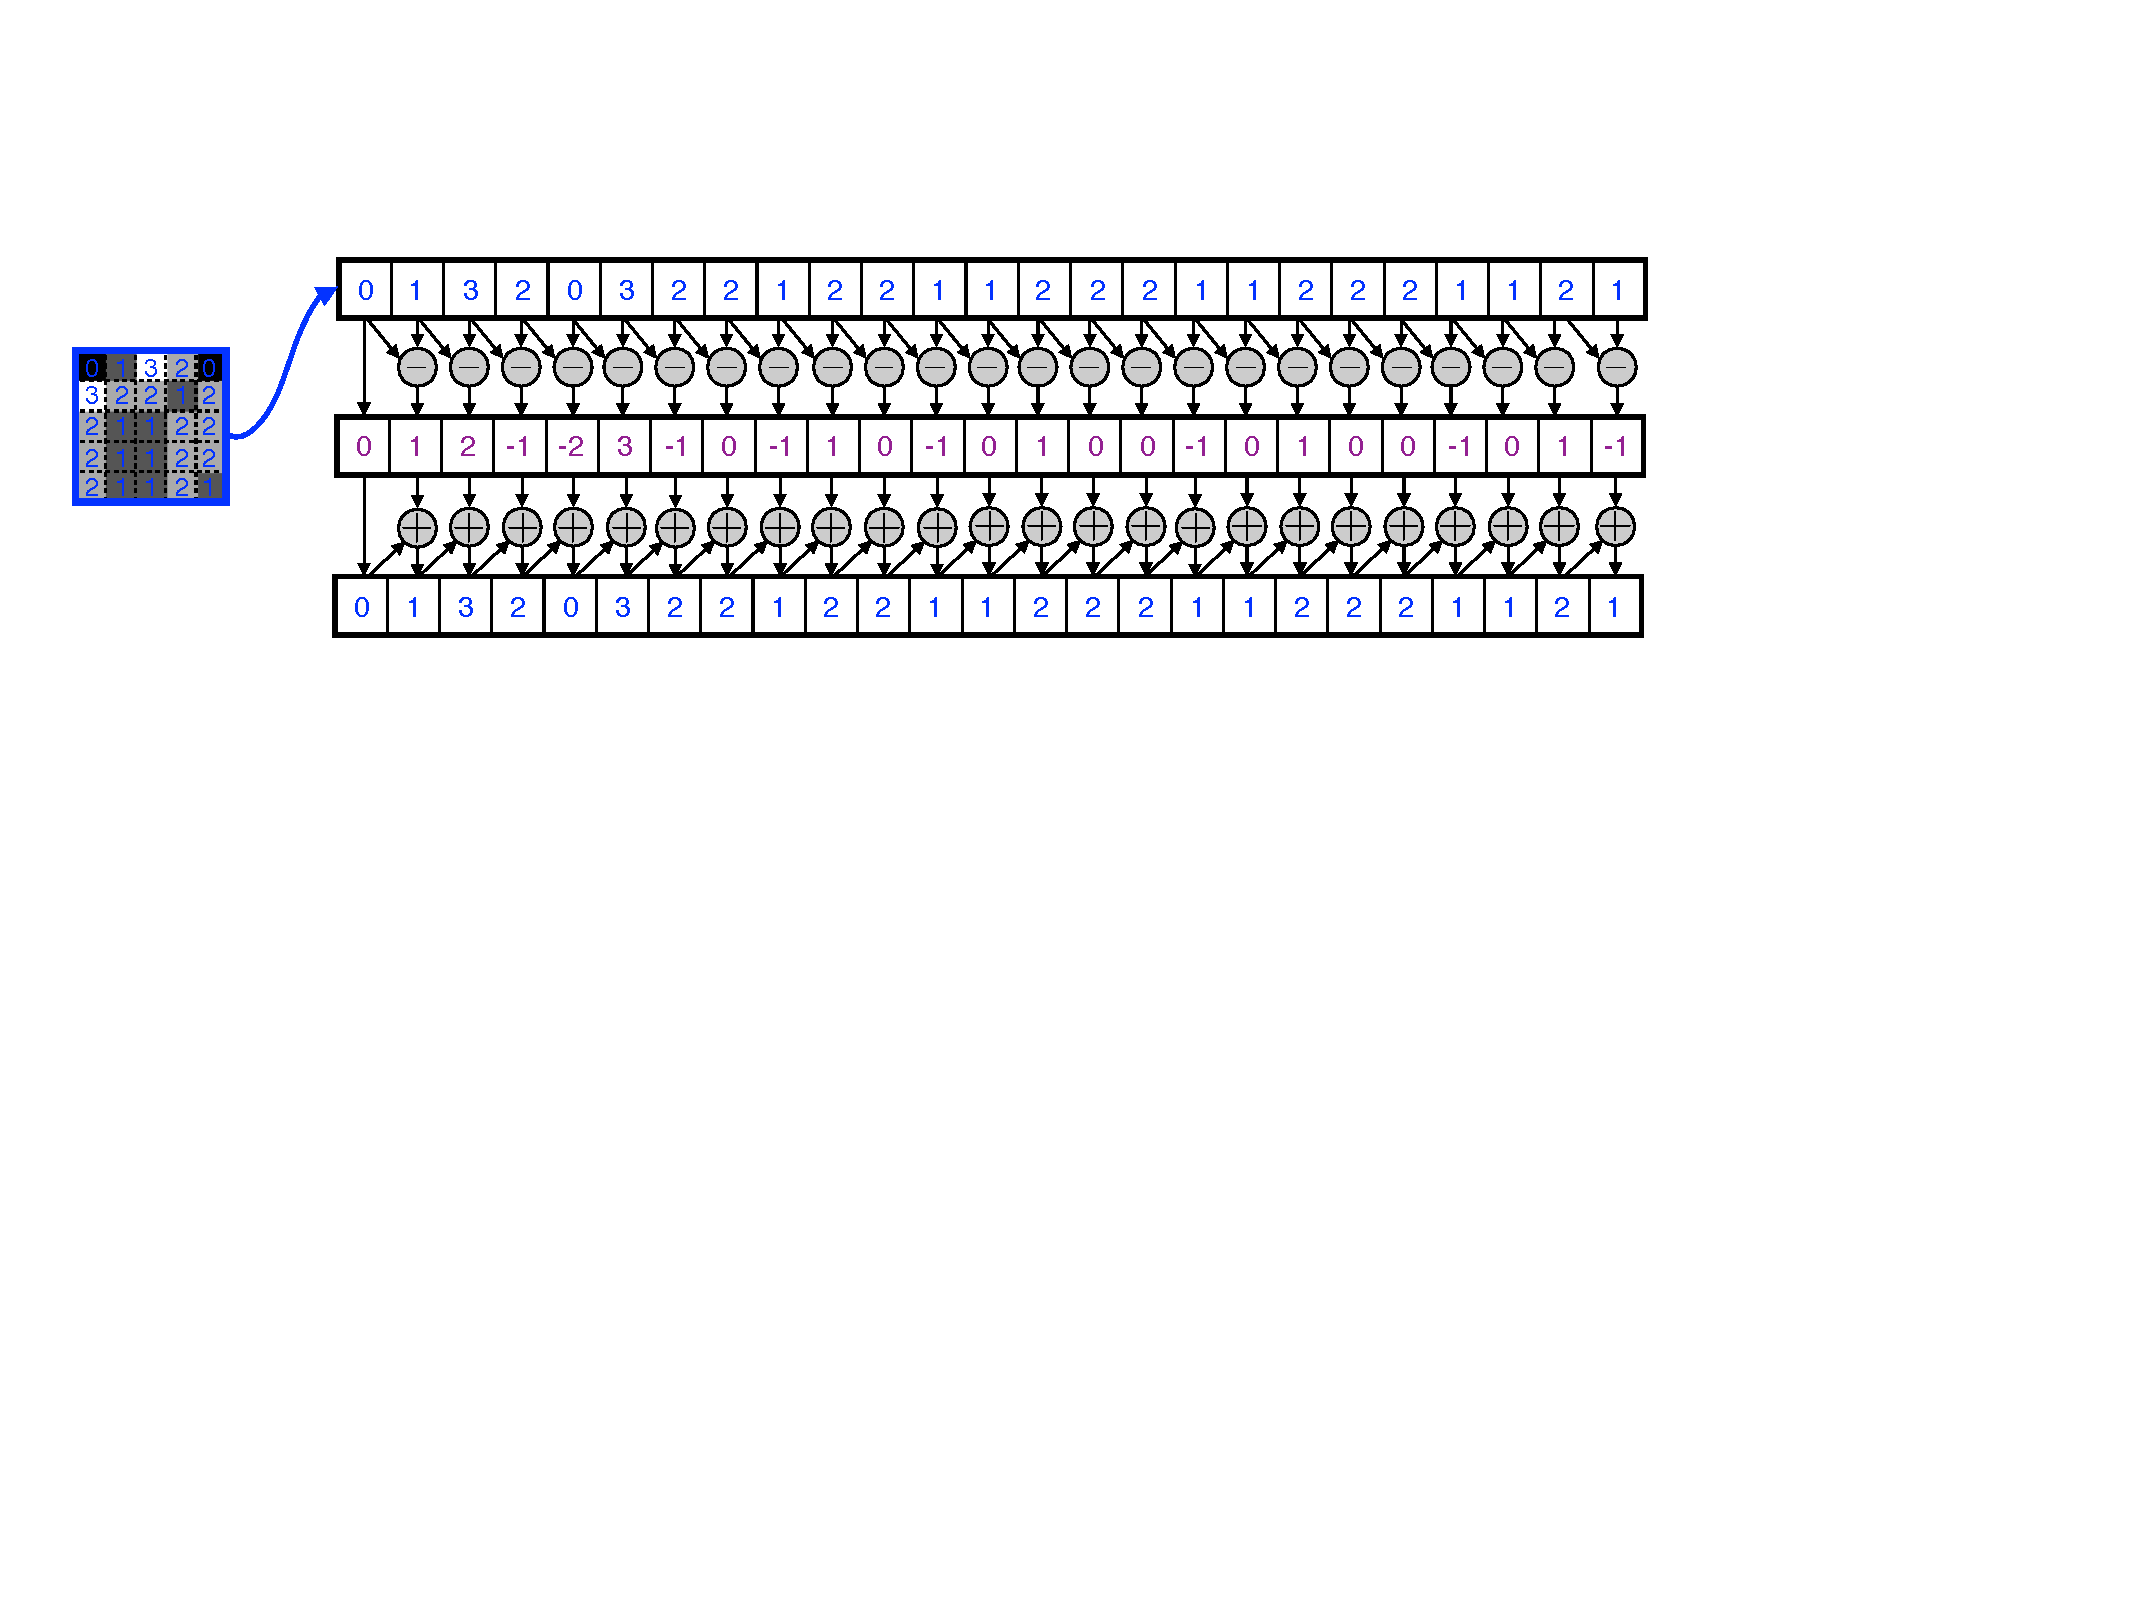
\includegraphics[width=.8\linewidth]{1-shannon/differences/differences}
%
\tabtrois{
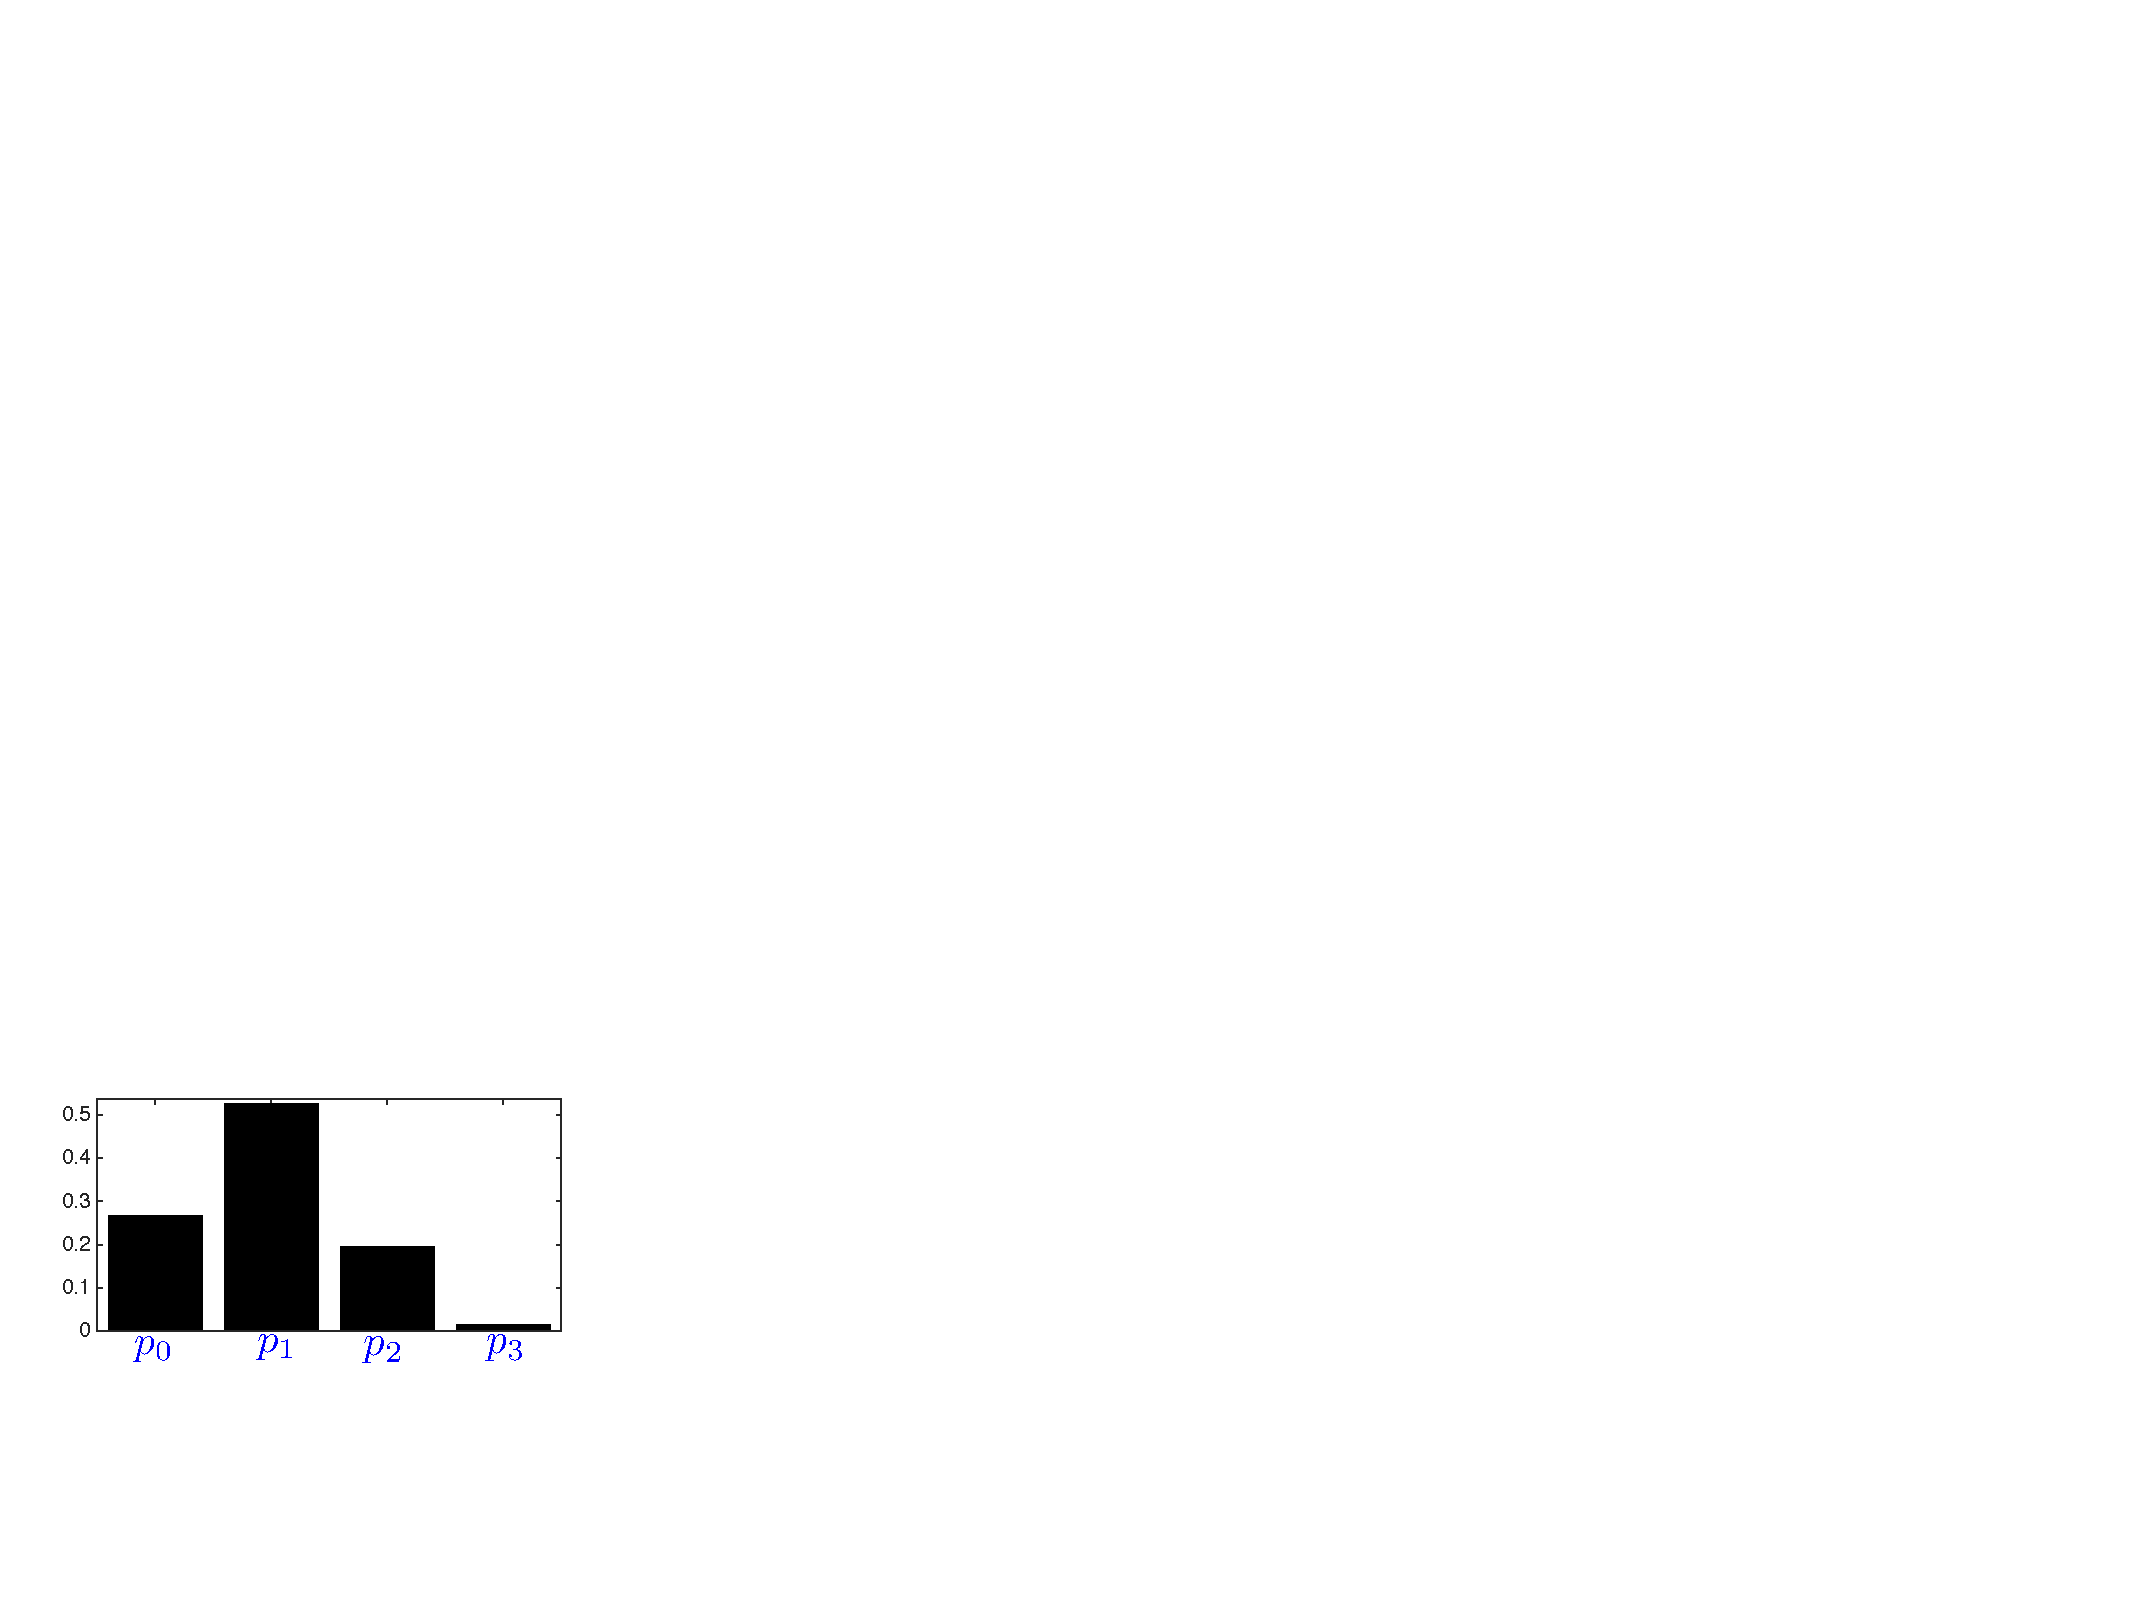
\includegraphics[width=.25\linewidth]{1-shannon/differences/histo-pix}&
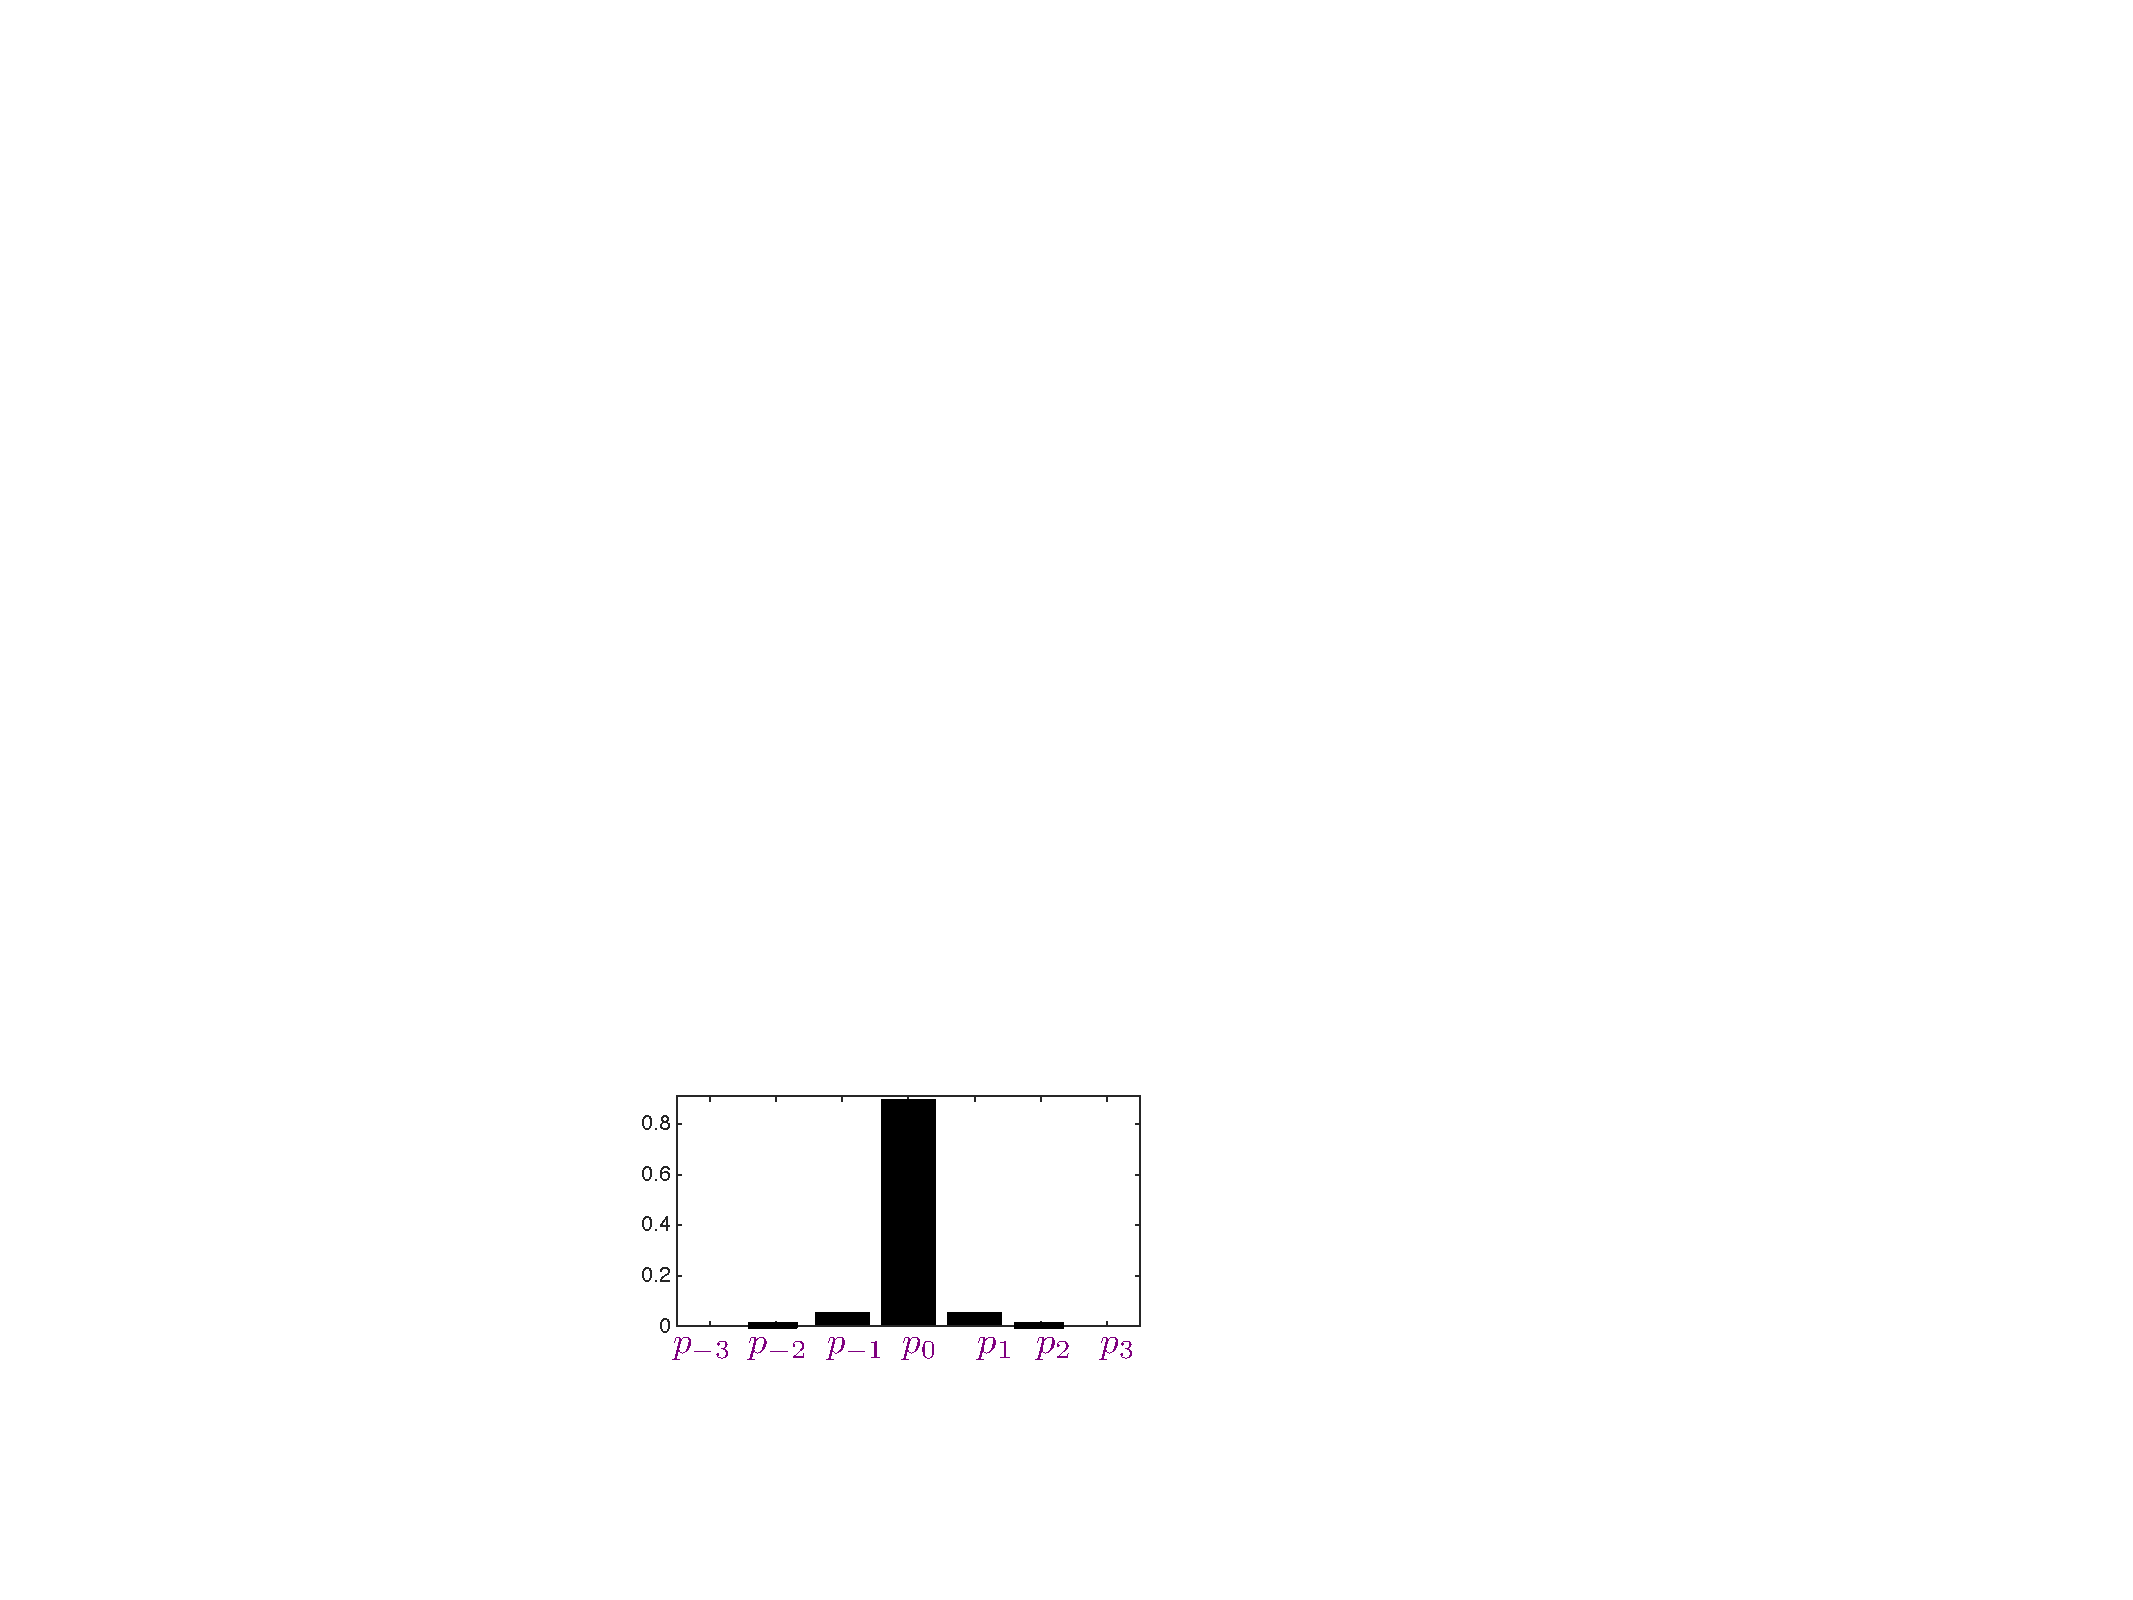
\includegraphics[width=.25\linewidth]{1-shannon/differences/histo-diff}&
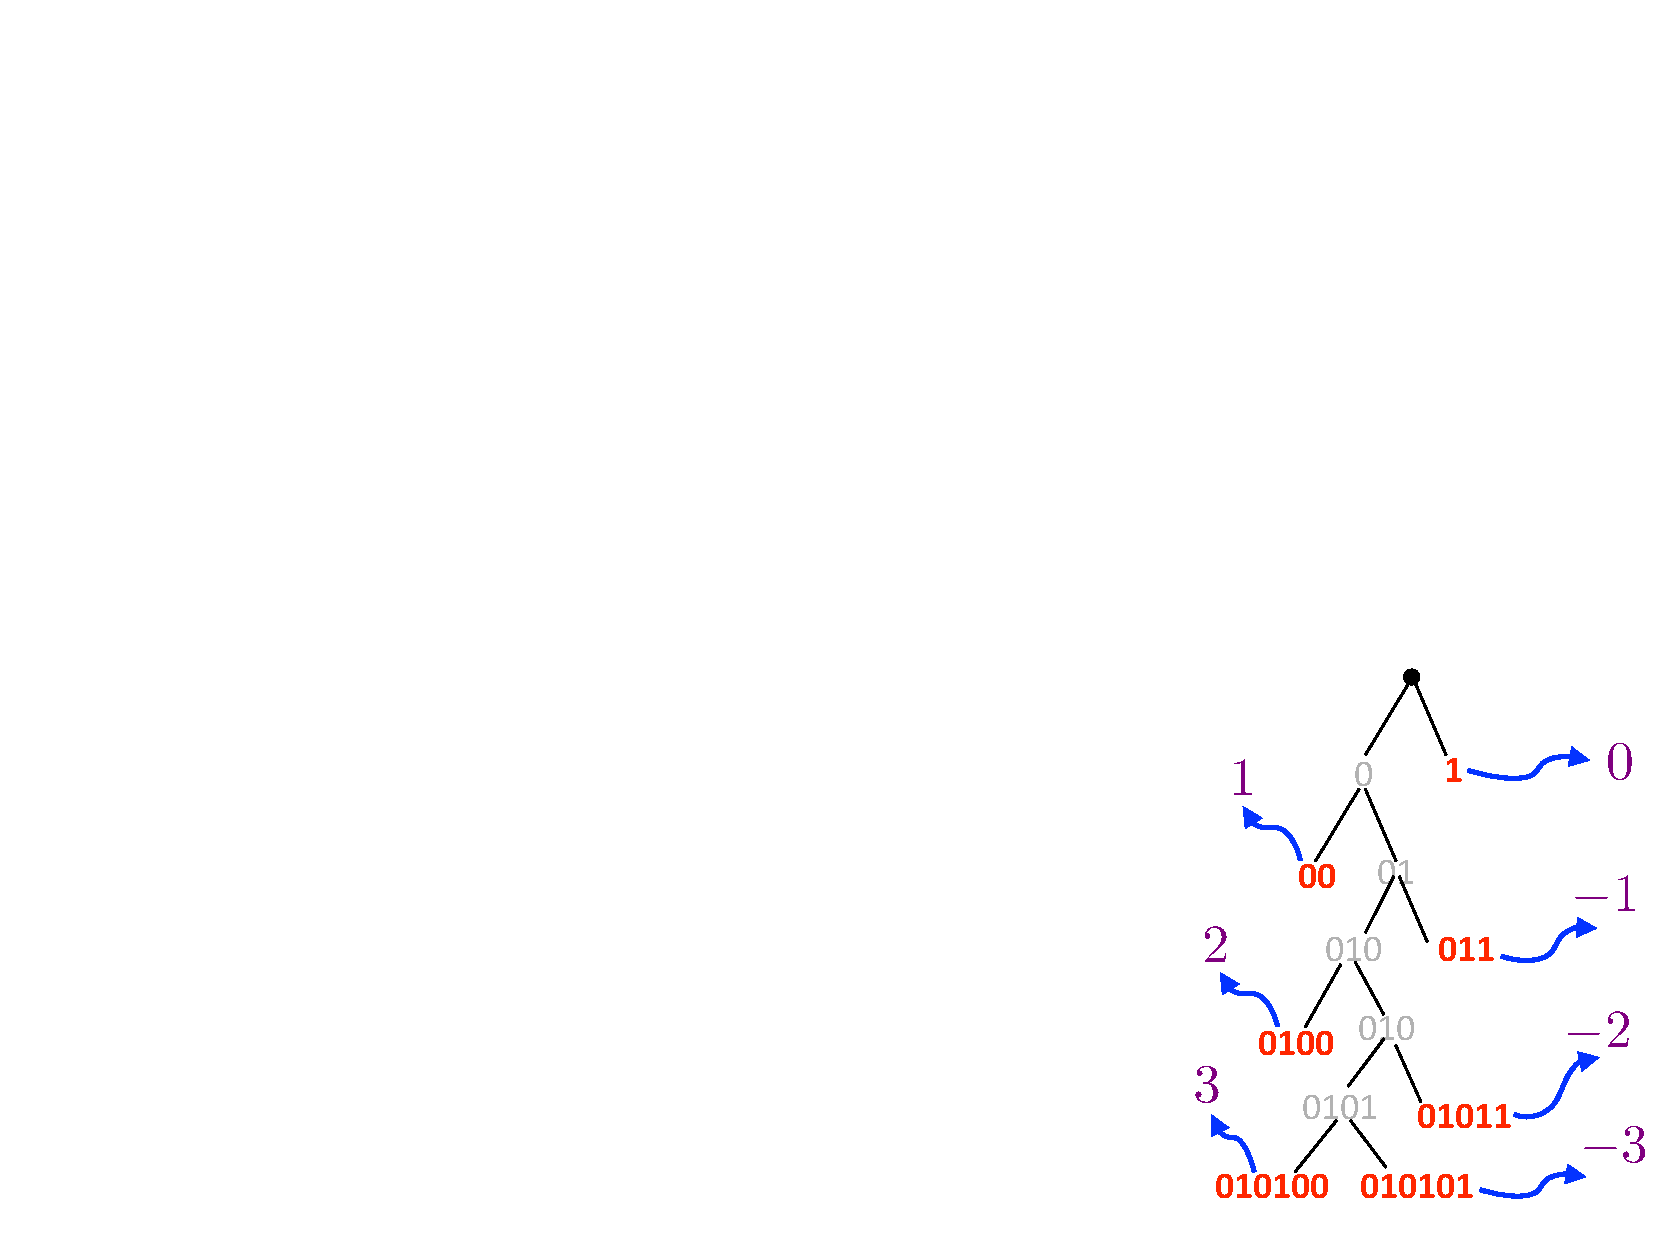
\includegraphics[width=.2\linewidth]{1-shannon/differences/arbre-difference}\\
$H(p) \approx 1.54, L(c) \approx 1.67 $ & $H(p) \approx 0.61, L(c) \approx 1.16 $ & Coding Tree
}
}{Top: retransformation by successive differences.
%
Bottom: comparison of histograms of pixel values and differences, and a code tree for these differences.
%
}{fig-codage-differences}

Another, more systematic way to leverage such temporal redundancy is by performing run-length-coding, which operate by grouping together sequence of similar symbols and thus coding first a symbol and then the length of the associated group (which is coded entropically). If the sequence is generated by a Markov chain, this method can be shown to asymptotically reach the Shannon bound where now the entropy is the entropy associated to the distribution of the Markov chain on infinite sequences (which can be computed as the limit of the entropy for finite sequences).




% !TEX root = ../IntroImaging.tex

\chapter{Image Processing}
\label{chap-images}

\newcommand{\FootLink}[1]{\footnote{\url{#1}}}
\newcommand{\myparagraph}[1]{\vspace{2mm}\noindent\textbf{#1}}
\newcommand{\lien}[2]{#2}

%\newcommand{\bs}{\_}

\newcommand{\BetweenImageSpace}{\hspace{3mm}}

\newcommand{\image}[1]{\includegraphics[width=0.32\linewidth]{#1}}
\newcommand{\imageM}[1]{\includegraphics[width=0.4\linewidth]{#1}}
\newcommand{\imageL}[1]{\includegraphics[width=0.6\linewidth]{#1}}
\newcommand{\imageQuad}[8]{
\begin{tabular}{@{}c@{\BetweenImageSpace{}}c@{}}
\image{#1} & \image{#2}\\
#5 & #6 \\
\image{#3} & \image{#4}\\
#5 & #6 
\end{tabular}
}
\newcommand{\imageTri}[6]{
\begin{tabular}{@{}c@{\BetweenImageSpace{}}c@{\BetweenImageSpace{}}c@{}}
\image{#1} & \image{#2} & \image{#3}\\
#4 & #5 & #6 \\
\end{tabular}
}
\newcommand{\imageDuo}[4]{
\begin{tabular}{@{}c@{\BetweenImageSpace{}}c@{}}
\image{#1} & \image{#2} \\
#3 & #4  \\
\end{tabular}
}

\newcommand{\myfigure}[3]{
    \begin{figure}[ht]
    \begin{center}
        #1                          % usual include graphics
    \end{center}
    \vspace{-4mm}
        \caption{\textit{#2}}       % caption
    \label{#3}          % label
    \end{figure}
}



Digital cameras take precise photographs of the world around us. The user wants to be able to store his photos on his hard drive with minimum memory requirement. He also wishes to be able to reprocess them in order to improve their quality. This article presents the mathematical and computer tools used to perform these different tasks. 

%%%%%%%%%%%%%%%%%%%%%%%%%%%%%%%%%%%%%%%%%%%%%%%%%%%%%%%%%%%%%%
%%%%%%%%%%%%%%%%%%%%%%%%%%%%%%%%%%%%%%%%%%%%%%%%%%%%%%%%%%%%%%
%%%%%%%%%%%%%%%%%%%%%%%%%%%%%%%%%%%%%%%%%%%%%%%%%%%%%%%%%%%%%%
\section{The pixels of an image}

A \lien{https://en.wikipedia.org/wiki/Digital_image}{digital image}
in gray levels is an array of values. Each
box of this table, which stores a value, is called a
\lien{https://en.wikipedia.org/wiki/Pixel}{pixel}.
By noting $n$ the number of rows and $p$ the number of columns in the image,
we manipulate an array of $n \times p$ pixels. Figure \ref{fig-section1-original-zoom}, left, shows a visualization of a square table with $n = p = 240$, which represents $240\times 240$ = 57600 pixels. The
\lien{https://en.wikipedia.org/wiki/Digital_camera}{digital cameras}
can record much larger images,
with several millions of pixels.

The values of the pixels are stored in
\lien{http://en.wikipedia.org/wiki/Computer}{a computer} or
a digital camera in the form of
\lien{https://en.wikipedia.org/wiki/Integer}{relative integers} between entre 0 et $255=2^8-1$,
making 256 possible values for each pixel. The value 0 is black, and the value 255 is white. The intermediate values correspond to
\lien{https://en.wikipedia.org/wiki/Grayscale}{gray levels}
ranging from black to white. Figure \ref{fig-section1-original-zoom} shows a subset of $6 \times 6$ pixels taken from the previous image. You can see both the values that make up the table and the gray levels that allow you to display the image on the screen.

\myfigure{
\imageL{section1-original-zoom}
}{Sub-image of size $5 \times 5$}{fig-section1-original-zoom}

%%%%%%%%%%%%%%%%%%%%%%%%%%%%%%%%%%%%%%%%%%%%%%%%%% %%%%%%%%%%%%
%%%%%%%%%%%%%%%%%%%%%%%%%%%%%%%%%%%%%%%%%%%%%%%%%% %%%%%%%%%%%%
\section{Image Storage}

%%%%%%%%%%%%%%%%%%%%%%%%%%%%%%%%%%%%%%%%%%%%%%%%%% %%%%%%%%%%%%
\subsection{Binary Codes}

Storing large images on the
\lien{https://en.wikipedia.org/wiki/Hard_disk_drive}{hard drive}
of a computer takes
a significant amount of places. Integer numbers are stored
in \lien{https://en.wikipedia.org/wiki/Binary_number}{binary},
in the form of a succession
of 0 and 1. Each 0 and each 1 corresponds to an elementary unit
of information, called bit.
To obtain the binary expression of a pixel having the value 179,
it is necessary to decompose this value as a sum of powers of two.
We thus obtain
\[ 
	179=2^7+2^5+2^4+2+1, 
\]
where care has been taken to order the powers of two in decaying order. In order to make the binary more explicit,
we add ``$1 \times$" before each power that appears in the expression,
and ``$0\times$" before the powers that do not appear
\[ 179=1 \times 2^7 + 0 \times 2^6 + 1 \times 2^5 + 1 \times 2^4 + 
  0 \times 2^3 + 0 \times 2^2 + 1 \times 2^1 + 1 \times 2^0. \]
Using such a decomposition, the value of each pixel, which is a number between 0 and 255, requires
$\log_2(256) = 8\text{bits}$. 
The binary writing of the value 179 of the pixel is thus $(1,0,1,1,0,0,1,1)$.
Any value between 0 and 255 can be written in this way, which requires the use of 8 bits. Indeed,
there are 256 possible values, and $256 = 2^8$. To store the complete image, it is therefore necessary to use $n \times p \times 8 \text{bits}$.
For the image shown in the previous figures, it is thus necessary to use
\[
	256 \times 256 \times 8 = 524288 \text{bits}. 
\]
Equivalently, this image requires 57.6kb (kilobytes), since a kilobyte is equal to $8$ bits.


%%%%%%%%%%%%%%%%%%%%%%%%%%%%%%%%%%%%%%%%%%%%%%%%%% %%%%%%%%%%%%
\subsection{Sub-sampling an Image}


\myfigure{
\imageTri
%{section2-subsample-2}
{section2-subsample-4}
{section2-subsample-8}
{section2-subsample-16}
%{Une ligne/colonne sur 2}
{One row / column of 4}
{One row / column out of 8}
{One row / column of 16}
}{Subsampling of an image}{fig-section2-subsample}

In order to reduce the required storage space of an image, the number of pixels can be reduced.
The easiest way to do this is to delete rows and columns in the original image. Figure \ref{fig-section2-subsample}, at the top left, shows what is obtained if one row is kept out of 4 and one column out of 4. We thus have divided by $4 \times 4 = 16$ the number of pixels of the image, and thus also divided by 16 the number of bits required to store the image on
a hard disc. In fig. \ref{fig-section2-subsample}, one can see the results obtained by removing more and more rows and columns. Of course, the quality of the image degrades quickly.

%%%%%%%%%%%%%%%%%%%%%%%%%%%%%%%%%%%%%%%%%%%%%%%%%% %%%%%%%%%%%%
\subsection{Quantizing an image}

Another way to reduce the memory space required for storage
is to use fewer integers for each value. For example, we can use only integers between 0 and 3, which will give an image with only 4 levels of gray. One can convert the original image to an image with 4 levels of values by performing the replacements:
\begin{rs}
\item the values in $0,1,\ldots, 63$ are replaced by the value 0 (black),
\item the values in $64,1,\ldots, 127$ are replaced by the value 1 (light gray),
The values in $128.1,\ldots, 191$ are replaced by the value 2 (dark gray),
\item the values in $192,\ldots, 255$ are replaced by the value 3 (white).
\end{rs}
Such an operation is called \lien{https://en.wikipedia.org/wiki/Quantization}{quantization}. Figure~\ref{fig-section3-quantize}, in the center, shows the resulting image with 4 grayscale levels.

We have already seen that we can represent any value between 0 and 255 using 8 bits using binary coding. In the same way,
one can check that any value between 0 and 3 can be represented using 2 bits.
This thus results in a reduction of a factor 8/2=4 of the memory footprint necessary
for storing the image on a hard disk. Figure \ref{fig-section3-quantize} shows the results obtained using less and less gray levels.

\myfigure{
\imageDuo
%{section3-quantize-2}
%{section3-quantize-3}
{section3-quantize-4}
{section3-quantize-16}
%{16 niveaux de gris}
%{3 niveaux de gris}
{4 gray levels}
{16 gray levels}
}{Quantizing an image
}{fig-section3-quantize}
 
As with the reduction of the number of pixels, the reduction of the number
gray levels greatly affects the quality of the image.
In order to minimize the size of an image without changing its quality,
more complex methods of
\lien{https://en.wikipedia.org/wiki/Image_compression}{image compression}.
The most effective method is JPEG-2000. It uses the theory of wavelets.




%%%%%%%%%%%%%%%%%%%%%%%%%%%%%%%%%%%%%%%%%%%%%%%%%% %%%%%%%%%%%%
%%%%%%%%%%%%%%%%%%%%%%%%%%%%%%%%%%%%%%%%%%%%%%%%%% %%%%%%%%%%%%
%%%%%%%%%%%%%%%%%%%%%%%%%%%%%%%%%%%%%%%%%%%%%%%%%% %%%%%%%%%%%%
\section{Noise Removal}

%%%%%%%%%%%%%%%%%%%%%%%%%%%%%%%%%%%%%%%%%%%%%%%%%% %%%%%%%%%%%%
\subsection{Local Averaging}

Images are sometimes of poor quality. A typical example of a defect
is the noise which appears when a picture is under-exposed,
that is if there is not enough light. This noise corresponds to small
random fluctuations of the gray levels. Figure~\ref{fig-section5-moyenne}, on the left, shows such 
a noisy image.


\myfigure{
\imageM{section5-moyenne-numbers}
}{Pixels neighborhood.
}{fig-section5-moyenne-numbers}

In order to remove the noise in the images, it is necessary to
modify the pixel values.
The simplest operation is to replace the value
$a$ of each pixel by the average of
$a$ and the values $b, c, d, e, f, g, h, i$ of the 8 pixels that surround $a$. Figure \ref{fig-section5-moyenne-numbers} shows an example of a neighborhood of 9 pixels. A modified image is thus obtained by replacing $a$ by
\[\frac{a + b + c + d + e + f + g + h + i}{9}, \]
since the average of 9 values is averaged.
%
In our example, this average is
\[ \frac{190+192+79+54+47+153+203+189+166}{9} \approx 141. \]
By performing this operation for each pixel, a large part of 
the noise is removed, because this noise is made up of random fluctuations, which are
decreased by averaging. Figure \ref{fig-section5-moyenne}, top left, shows the effect of such a calculation. All the noise was not removed by this operation. In order to remove more
of noise, one can average more values around each pixel.
%
Figure \ref{fig-section5-moyenne} shows the result obtained by increasing the average
of values.


\myfigure{
\imageTri
{section5-moyenne-1}
{section5-moyenne-2}
{section5-moyenne-3}
%{section5-moyenne-4}
{Mean on 9 pixels}
{Mean on 25 pixels}
{Mean on 49 pixels}
%{Moyenne sur 81 pixels}
}{Mean with increasing width
}{fig-section5-moyenne}

Pixel averaging is very effective in removing noise in
images, unfortunately it also destroys much of the
the information of the image. It can indeed be seen that the images
obtained by averaging are blurry.
This is particularly visible near contours, which are not sharp.

%%%%%%%%%%%%%%%%%%%%%%%%%%%%%%%%%%%%%%%%%%%%%%%%%% %%%%%%%%%%%%
\subsection{Local Median}

To reduce this blur, the mean can be replaced by the median. In the example of the neighborhood of 9 pixels used in the previous section, the 9 sorted values are:
\[47, 54, 79, 153, 166, 189, 190, 192, 203. \]
The median of these nine values is 166. In order to remove more noise, it is enough to calculate the median over a larger number of neighboring pixels, as shown in Figure \ref{fig-section6-mediane}.
One can observe that this method is more efficient than the mean calculation 
because the resulting images are less blurry. However, just as
with the calculation of averages, if we take neighborhoods that are too large, we lose
also information of the image, especially the edges of the objects are degraded.


\myfigure{
\imageTri
{section6-mediane-1}
{section6-mediane-2}
{section6-mediane-3}
%{section6-mediane-4}
{Median on 9 pixels}
{Median on 25 pixels}
{Median on 49 pixels}
%{M�diane sur 81 pixels}
}{Median filtering with increasing windowing size.
}{fig-section6-mediane}




%%%%%%%%%%%%%%%%%%%%%%%%%%%%%%%%%%%%%%%%%%%%%%%%%% %%%%%%%%%%%%
%%%%%%%%%%%%%%%%%%%%%%%%%%%%%%%%%%%%%%%%%%%%%%%%%% %%%%%%%%%%%%
%%%%%%%%%%%%%%%%%%%%%%%%%%%%%%%%%%%%%%%%%%%%%%%%%% %%%%%%%%%%%%
\section{Detecting Edges of Objects}

In order to locate objects in the images, it is necessary to
detect their edges. These edges correspond to
areas of the image where pixel values change rapidly. It is the case
for example when passing from the boat (which is dark,
ie. with small values) to the sea (which is clear, therefore with
large values).

In order to know if a pixel with a value $a$ is along an edge of an object, the values $b, c, d, e$ of its four neighbors are taken into account, which have a common side with it (Figure \ref{fig-section7-contours-numbers}). This allows the edges of objects to be detected as accurately as possible.


\myfigure{
\imageM{section7-contours-numbers}
}{Example of a neighborhood of 5 pixels.
}{fig-section7-contours-numbers}


A value $\ell$ is calculated according to the formula
\[ \ell = \sqrt{ (b-d)^2 + (c-e)^2 }.  \]
In our example, we thus obtain
\[ \ell= \sqrt{�(192 - 153)^2 + (189 - 54)^2 } = \sqrt{19746} \approx 141. \]
It may be noted that if $\ell = 0$, then $b = c$
and $d = e$. On the contrary, if
$\ell$ is large, this means that the neighboring pixels have very high values
different, the pixel considered is therefore probably on the edge of an object.

Figure \ref{fig-section7-contours} shows an image whose pixel value is $\min(\ell, 255)$.
It is necessary to take the minium with 255, because the value of $\ell$ can exceed the maximum displayable value (255, which corresponds to white). These values are displayed with black when $\ell = 0$, in white when $\ell$ is high, and gray levels are used for the intermediate values. It can be seen that in the image on the right, the outlines of the objects appear white, as they correspond to  large values of $\ell$.

\myfigure{
\imageDuo
{section7-image}
{section7-contours}
{Original Image}
{Contour map $\ell$}
}{Edge detection.
}{fig-section7-contours}

%%%%%%%%%%%%%%%%%%%%%%%%%%%%%%%%%%%%%%%%%%%%%%%%%%%%%%%%%%%%%%
%%%%%%%%%%%%%%%%%%%%%%%%%%%%%%%%%%%%%%%%%%%%%%%%%%%%%%%%%%%%%%
%%%%%%%%%%%%%%%%%%%%%%%%%%%%%%%%%%%%%%%%%%%%%%%%%%%%%%%%%%%%%%
\section{Color Images}


%%%%%%%%%%%%%%%%%%%%%%%%%%%%%%%%%%%%%%%%%%%%%%%%%% %%%%%%%%%%%%
\subsection{RGB Space}

A
\lien{https://en.wikipedia.org/wiki/Color_space}{color image}
is actually composed of three independent images,
in order to represent the
\lien{https://en.wikipedia.org/wiki/RGB_color_model}{red, green, and blue}.
Each of these three
images is called a
\lien{https://en.wikipedia.org/wiki/Channel_(digital_image)}{color channel}.
This representation in red, green and blue mimics the
human visual system.
Figure~\ref{fig-canaux-coul} shows the three constituent channels of the image shown on the left of Figure~\ref{fig-luminance}.

\myfigure{
\imageDuo
{section8-image}
{section8-luminance}
{Original image}
{Luminance}
}{Color image.
}{fig-luminance}


Each pixel of the color image thus contains three numbers $(r, v, b)$,
each being an integer between 0 and 255.
If the pixel is equal to $(r, v, b) = (255,0,0)$, it contains only information
red, and is displayed as red.
Similarly, the pixels of $(0,255,0)$ and $(0,0,255)$ are
respectively displayed green and blue.


\myfigure{
\imageTri
{section8-rouge}
{section8-vert}
{section8-bleu}
{Red canal }
{Green canal}
{Blue canal}
}{Color channels
}{fig-canaux-coul}


A color image can be displayed on the screen.
from its three channels $(r, v, b)$ using the rules of
\lien{https://en.wikipedia.org/wiki/Additive_color}{additive color synthesis}. These rules correspond to the way in which light rays combine, hence the qualifier \guill{additive}.
Figure \ref{fig-section8-synthese}, left, shows the composition rules
this additive synthesis of colors.
For example, a pixel with the values
$(r, v, b) = (255,0,255)$ is a mixture of red and green,
displayed as yellow.


\myfigure{
\imageDuo
{section8-synthese-additive}
{section8-synthese-soustractive}
{Additive synthesis}
{Subtractive synthesis}
}{Color Synthesis
}{fig-section8-synthese}


%%%%%%%%%%%%%%%%%%%%%%%%%%%%%%%%%%%%%%%%%%%%%%%%%% %%%%%%%%%%%%
\subsection{CMJ Space}

Another common representation for color images uses
as background colors cyan, magenta and yellow. It is calculated
the three numbers $(c, m, j)$ corresponding to each of these three channels
from the red, green and blue channels $(r, v, b)$ as follows
\[c = 255-r, \quad m = 255-v, \quad j = 255-b. \]
For example, a pixel of pure blue
$(r, v, b) = (0,0,255)$ will become
$(c, m, j) = (255,255,0)$. Figure~\ref{fig-canaux-cmj} shows the three channels
$(c, m, j)$ of a color image.

\myfigure{
\imageTri
{section8-cyan}
{section8-magenta}
{section8-jaune}
{Cyan canal}
{Magenta canal}
{Yellow canal}
}{Channels CMJ
}{fig-canaux-cmj}


In order to display a color image on the screen from the three channels $(c, m, j)$, the \lien{https://en.wikipedia.org/wiki/Subtractive_color}{subtractive color synthesis} must be used. Figure \ref{fig-section8-synthese}, right, shows the composition rules of this subtractive synthesis. They correspond in painting to the absorption of light by colored pigments, hence the qualifier \guill{subtractive}. Cyan, magenta and yellow are called primary colors.

It is thus possible to store on a hard disk a color image by storing the
three channels, corresponding to the $(r, g, b)$ or $(c, m, j)$.
%
One can change color images in a similar way as graylevel image, by changing each channel.


%%%%%%%%%%%%%%%%%%%%%%%%%%%%%%%%%%%%%%%%%%%%%%%%%%%%%%%%%%%%%%
%%%%%%%%%%%%%%%%%%%%%%%%%%%%%%%%%%%%%%%%%%%%%%%%%%%%%%%%%%%%%%
%%%%%%%%%%%%%%%%%%%%%%%%%%%%%%%%%%%%%%%%%%%%%%%%%%%%%%%%%%%%%%
\section{Changing the Contrast of an Image}

%%%%%%%%%%%%%%%%%%%%%%%%%%%%%%%%%%%%%%%%%%%%%%%%%% %%%%%%%%%%%%
\subsection{Luminance}

One calculates a grayscale image from a color image
as the mean of the three channels. Thus, for each pixel, a value
\[a = \frac{r + v + b}{3} \]
is computed which is called luminance
of the color. Figure \ref{fig-luminance} shows the transition from a color image to a luminance image in grayscales. 


%%%%%%%%%%%%%%%%%%%%%%%%%%%%%%%%%%%%%%%%%%%%%%%%%% %%%%%%%%%%%%
\subsection{Grayscale contrast manipulations}

It is possible to make various changes to the image in order to
modify his contrast. We consider here a grayscale image.
A simple manipulation consists in replacing each value $a$ of a pixel of an image by $255-a$, which corresponds to the opposite gray intensity. The white becomes black and vice-et-versa, giving a similar effect to that
of the negative of film for cameras, see figure \ref{fig-section4-square}, left.

The image is lightened or darkened using an increasing function from $[0,255]$ to itself, which is applied to the $a$ values of the pixels. One can darken the image by using the square function. More precisely, we define the new value of a pixel of the image as $a^2/255$ (see figure \ref{fig-section4-square} in the center). Since the result is not generally an integer, it is rounded to the nearest integer. Similarly, for lightening the image, the value $a$ of each pixel is replaced by the rounding of $\sqrt{255 a} $. Figure \ref{fig-section4-square}, on the right, shows the obtained result. It will be noted that these two operations (square lightening and square root darkening) are inverse to one another.

% It will be noted that these two operations (square lightening and square root darkening) are inverse to one another.


\myfigure{
\imageTri{section4-negatif}
{section4-square}
{section4-sqrt}
{Negative}
{Square}
{Square root}
}{Changing the contrast.
}{fig-section4-square}


%%%%%%%%%%%%%%%%%%%%%%%%%%%%%%%%%%%%%%%%%%%%%%%%%% %%%%%%%%%%%%
\subsection{Manipulations of Color Contrast}

In order to manipulate the contrast of a color image, it is important to respect the color tones as much as possible. It is therefore simpler to manipulate only the luminance component $a = (r + v + b) / 3$, while maintaining the residue $(r-a, v-a, b-a)$ constant. For example, a change in contrast can be defined by raising the luminance $a$ to the $\ ga> 0$ in order to obtain
\[
	\tilde a = 255 \times \pa{ \frac{a}{255} }^{\ga} = 255 \times \text{exp}\pa{  \ga \times \text{ln}
		\pa{ \frac{a}{255} }  },
\]
(with Convention $\tilde a = 0$ when $a = 0$). It is noted that for $\ga = 1/2$ (respectively $\ga = 2$) the contrast change is found by squaring (respectively square root) introduced in the previous section. And of course, for $\ga = 1$, the luminance is unchanged.

% As $\ga$ is not necessarily an integer, it is important to use the exponential and the logarithm to define this change.

This change in contrast is then reflected on the color image by defining three channels $(\tilde r, \tilde v, \tilde b)$ of a new image by
\[
	\choice{
	\tilde r = \max(0, \min(255, r + \tilde a - a)),\\ 
	\tilde v = \max(0, \min(255, v + \tilde a - a)),\\
	\tilde b = \max(0, \min(255, b + \tilde a - a)).
	}	
\]
It is important to take the maximum with 0 and the minimum with 255 so that the result remains in the range $[0.255]$, and is displayed correctly. Figure \ref{fig-contrast-color} shows the result for different values of $\ga$. For $\ga <1$, the image looks clearer, while for $\ga> 1$, the image is darkened.

\newcommand{\imgsix}[1]{\includegraphics[width=0.16\linewidth]{#1}}

\myfigure{
\begin{tabular}{@{}c@{\hspace{1mm}}c@{\hspace{1mm}}c@{\hspace{1mm}}c@{\hspace{1mm}}c@{\hspace{1mm}}c@{}}
\imgsix{section4-constrast-1}&
\imgsix{section4-constrast-2}&
\imgsix{section4-constrast-3}&
\imgsix{section4-constrast-4}&
\imgsix{section4-constrast-5}&
\imgsix{section4-constrast-6}\\
$\ga=0,5$& 
$\ga=0,75$&
$\ga=1$&
$\ga=1,5$&
$\ga=2$&
$\ga=3$
\end{tabular}
}{Changing the contrast of a color image.
}{fig-contrast-color}





%%%%%%%%%%%%%%%%%%%%%%%%%%%%%%%%%%%%%%%%%%%%%%%%%%%%%%%%%%%%%%
%%%%%%%%%%%%%%%%%%%%%%%%%%%%%%%%%%%%%%%%%%%%%%%%%%%%%%%%%%%%%%
%%%%%%%%%%%%%%%%%%%%%%%%%%%%%%%%%%%%%%%%%%%%%%%%%%%%%%%%%%%%%%
\section{Images and Matrices}

%%%%%%%%%%%%%%%%%%%%%%%%%%%%%%%%%%%%%%%%%%%%%%%%%% %%%%%%%%%%%%
\subsection{Symmetry and Rotation}

An image is an array of numbers, with $n$ lines and $p$
columns. It is therefore easy to perform
some
\lien{https://en.wikipedia.org/wiki/Geometric_transformation}{geometric transformations}
on the image. The values of the pixels that make up this table (denoted $A$) can be
represented as $A = (a_{i,j})_{i,j}$
or index $i$ describes the set of numbers $\{1,\dots, n\}$
(the integers between 1 and n) and the index
$j$ the numbers $\{1,\dots, p\}$.
$a_{i,j}$ is said to be the value of the pixel at position $(i,j)$.

The array of pixels thus indexed is represented as
\[
A = 
\begin{pmatrix}
a_{1,1} &           &           &   & a_{1,p}\\
       &           &  \vdots   &   &  \\
	   &           & a_{i-1,j} &   & \\
\ldots & a_{i,j-1} & a_{i,j}   & a_{i,j+1} & \ldots\\
	   &           & a_{i+1,j} &   & \\
       &           &  \vdots   &   &  \\
a_{n,1} &           &           &   & a_{n,p}\\
\end{pmatrix},
\]
This corresponds to the representation of the image in the form of a matrix. Transposing this matrix corresponds to symmetry with respect to the main diagonal. This transposition is carried out on each of the three color components (see figure \ref{fig-geometric}, on the left).


\myfigure{
\imageTri
{section10-original}
{section10-transpose}
{section10-rotation}
{Matrice $A$}
{Matrix $B$ (transposed)}
{Matrix $C$ (rotation)}
}{Transpose and rotate.
}{fig-geometric}

It is also possible to carry out a rotation by
a quarter turn clockwise on the image. This is obtained by defining a matrix $C = (c_{i,j})_{j, i}$ of
$p$ lines and $n$
columns by $c_{j, i} = a_{n-i+1,j} $.
Figure \ref{fig-geometric}, right, shows the action of this rotation on an image.



%%%%%%%%%%%%%%%%%%%%%%%%%%%%%%%%%%%%%%%%%%%%%%%%%%%%%%%%%%%%%%
\subsection{Interpolation Between Two Images}

It is possible to carry out a
\lien{https://en.wikipedia.org/wiki/Dissolve_(filmmaking)}{transition between two images}
$A$ and $B$. It is therefore assumed that the two images have the same number $n$ of lines
and the same number $p$ of columns. $A = (a_{i,j})_{i,j}$ the pixels of image $A$ and
$B = (b_{i,j})_{i,j}$ the pixels of the image $B$.

For a value $t$ set between $0$ and $1$, the image
$C = (c_{i,j})_{i,j}$ is defined as
\[c_{i,j} = (1-t) a_{i,j} + t b_{i,j} .\]
It is the formula of a
\lien{https://en.wikipedia.org/wiki/Linear_interpolation}{linear interpolation}
between the two images. For a color image, this formula is applied to each of the
channels R, V and B.


It can be seen that for $t = 0$, the image $C$ is equal to the image
$A$. For $t = 1$, the image $C$ is equal to the image
$B$. When the value $t$ increases from 0 to 1, one thus obtains a fading
effect, since the image, which at first is close to image $A$
resembles more and more the image $B$. Figure \ref{fig-interp} shows the result obtained for 6 values of $t$ distributed between 0 and 1.

\myfigure{
\begin{tabular}{@{}c@{\hspace{1mm}}c@{\hspace{1mm}}c@{\hspace{1mm}}c@{\hspace{1mm}}c@{\hspace{1mm}}c@{}}
\imgsix{section11-interp-1}&
\imgsix{section11-interp-2}&
\imgsix{section11-interp-3}&
\imgsix{section11-interp-4}&
\imgsix{section11-interp-5}&
\imgsix{section11-interp-6}\\
Image $A$, t=0 & 
t=0.2 &
t=0.4 &
t=0.6 &
t=0.8 &
Image $B$, t=1
\end{tabular}
}{Linear interpolation.
}{fig-interp}



%%%%%%%%%%%%%%%%%%%%%%%%%%%%%%%%%%%%%%%%%%%%%%%%%% %%%%%%%%%%%%
%%%%%%%%%%%%%%%%%%%%%%%%%%%%%%%%%%%%%%%%%%%%%%%%%% %%%%%%%%%%%%
%%%%%%%%%%%%%%%%%%%%%%%%%%%%%%%%%%%%%%%%%%%%%%%%%% %%%%%%%%%%%%
\section*{Conclusion}

Mathematical processing of images is a very active field, where the theoretical advances are obtained using fast computational algorithms. These algorithms have important applications for the manipulation of digital contents. This article, however, only scratched the surface of the immense list of treatments that can be subjected to an image. We refer to the website \textit{A Numerical Tour of Signal Processing}\FootLink{http://www.numerical-tours.com/} for many more examples of image processing and links to other resources available online.


%%%%%%%%%%%%%%%%%%%%%%%%%%%%%%%%%%%%%%%%%%%%%%%%%%%%%%%%%%%%%%
%%%%%%%%%%%%%%%%%%%%%%%%%%%%%%%%%%%%%%%%%%%%%%%%%%%%%%%%%%%%%%
%%%%%%%%%%%%%%%%%%%%%%%%%%%%%%%%%%%%%%%%%%%%%%%%%%%%%%%%%%%%%%

\section*{Glossary}

\newcommand{\gloss}[1]{\item \textbf{#1}}

\begin{rs}
\gloss{random}: unpredictable value, such as noise disturbing images of bad qualities.
\gloss{Bit}: a basic unit for storing information in the form of 0 and 1 in a computer.
\gloss{Channel}: one of three elementary images that make up a color image.
\gloss{Edges}: the area of an image where the values of the pixels change rapidely, which corresponds to the contours of the objects that make up the image.
\gloss{Noise}: small perturbations that degrade the quality of an image.
\gloss{Square}:  the square $b$ of a value $a$ is $a \times a$. It is noted $a^2$.
\gloss{Contrast}: informal quantity that indicates how much difference there is between light and dark areas of an image.
\gloss{Image compression}: a method to reduce the amount of memory required to store an image on the hard disk.
\gloss{Binary coding}: writing of numeric values using only 0 and 1.
\gloss{Blur}: degradation of an image that makes the contours of objects unclear, and therefore difficult to locate precisely.
\gloss{Fade}: linear interpolation between two images.
\gloss{Color image}: a set of three grayscale images, which can be displayed on a color screen.
\gloss{Digital image}: an array of values that can be displayed on the screen by assigning a gray level to each value.
\gloss{Inverse}: operation that returns an image to its original state.
\gloss{JPEG-2000}: recent image compression method that uses a wavelet transform.
\gloss{Luminance}: average of the different channels in an image, which indicates the light output of the pixel.
\gloss{Matrix}: array of values, represented as $(a_{i,j})_{i,j}$.
\gloss{Median}: central value when sorting a set of values.
\gloss{Average}: the average of a set of values is their sum divided by their number.
\gloss{Grayscale}: grayscale used to display a digital image on the screen.
\gloss{integers}: numbers 0, 1, 2, 3, 4 ...
\gloss{Byte}: set of eight consecutive bits.
\gloss{Wavelets}: image transformation that is used by image compression JPEG-2000 method.
\gloss{Ascending order}: classifying a set of values from the smallest to the largest.
\gloss{Pixel}: a single element in the array of values that corresponds to a digital image.
\gloss{Quantization}: a method to reduce the set of possible values of a digital image.
\gloss{square root}: the square root $b$ of a positive value $a$ is the positive value $b$ such that $a = b \times b$. It is denoted $\sqrt{a}$.
\gloss{Resolution}: the size of an image (number of pixels).
\gloss{Exposed}: photograph of a scene too dark for which the photographic lens did not stay open long enough.
\gloss{Additive synthesis}: rule to construct any color from the three colors red, green and blue. This is the rule that governs the mixing of the colors of light beams when  illuminating a white wall.
\gloss{Subtractive synthesis}: rule to construct any color from the three cyan, magenta and yellow colors. This is the rule that governs the mixing of colors in paint.
\end{rs}
 


% !TEX root = ../IntroImaging-FR.tex


\chapter{Parcimonie, probl�mes inverses et �chantillonnage compress�}
\label{chap-sparsity}



Les standards actuels pour compresser de la musique, de l'image ou de la vid�o (MP3, JPG ou MPEG) utilisent tous des m�thodes issues de l'approximation non-lin�aire. Ces m�thodes calculent une approximation des donn�es initiales � l'aide d'une combinaison lin�aire d'un faible nombre de fonctions �l�mentaires (comme par exemple des sinuso�des ou des ondelettes). 
%
Ces m�thodes, initialement utilis�es pour l'approximation, le d�bruitage ou la compression, ont �t� appliqu�es plus r�cemment � des probl�mes plus difficiles, tels que l'augmentation de la r�solution ou l'inversion d'op�rateurs en imagerie m�dicale. Ces extensions n�cessitent la r�solution de probl�mes d'optimisation de grande dimension, et sont le sujet d'une intense activit� de recherche.
%
Une des derni�res avanc�es dans ce domaine, l'�chantillonnage compress�, utilise la th�orie des matrices al�atoires afin d'obtenir des garanties th�oriques pour la performance de ces techniques. L'�chantillonnage compress� permet d'envisager sous un angle nouveau la th�orie de l'�chantillonnage et de la compression de Claude Shannon. La compressibilit� des donn�es autorise en effet d'effectuer simultan�ment l'�chantillonnage et la compression des donn�es. 

Cet article pr�sente les concepts math�matiques cl�s qui ont permis l'�volution depuis l'�chantillonnage classique de Shannon vers l'�chantillonnage compress�. La notion de d�composition parcimonieuse, qui permet de formaliser l'id�e de compressibilit� de l'information, en est le fil directeur.



%%%%%%%%%%%%%%%%%%%%%%%%%%%%%%%%%%%%
\section{L'�chantillonnage classique}
\label{sec-echantillonnage}

Dans le monde num�rique, la plupart des donn�es (son, image, vid�o, etc.) sont discr�tis�es afin de les stocker, les transmettre et les modifier. 
%
A partir d'un signal \textit{analogique}, qui est repr�sent� par une fonction continue $s \mapsto \tilde f(s)$, l'appareil de mesure calcule un ensemble de $Q$ valeurs \textit{discr�tis�es} $f = (f_q)_{q=1}^Q \in \RR^Q$.
%
Ainsi, $Q$ est le nombre d'�chantillons temporels pour un morceau audio ou bien le nombre de pixels pour une image. 
%
La figure~\ref{fig-samples} montre des exemples de donn�es discr�tis�es.
%
Dans le cas d'une image, $\tilde f(s)$ repr�sente la quantit� de lumi�re arrivant en un point $s \in \RR^2$ du plan focal de l'appareil photo, et $f_q = \int_{c_q} \tilde f(s) \text{d} s$ est la quantit� de lumi�re totale illuminant la surface $c_q$ d'un capteur CCD index� par $q$. 
%
Pour simplifier, nous faisons ici l'hypoth�se de donn�es scalaires (par exemple un son mono,  une image ou une vid�o en niveaux de gris), mais les techniques d�crites ici peuvent s'�tendre au cas de donn�es vectorielles (son st�r�o, image couleur).


\begin{figure}\centering
\begin{tabular}{@{}c@{\hspace{5mm}}c@{}}
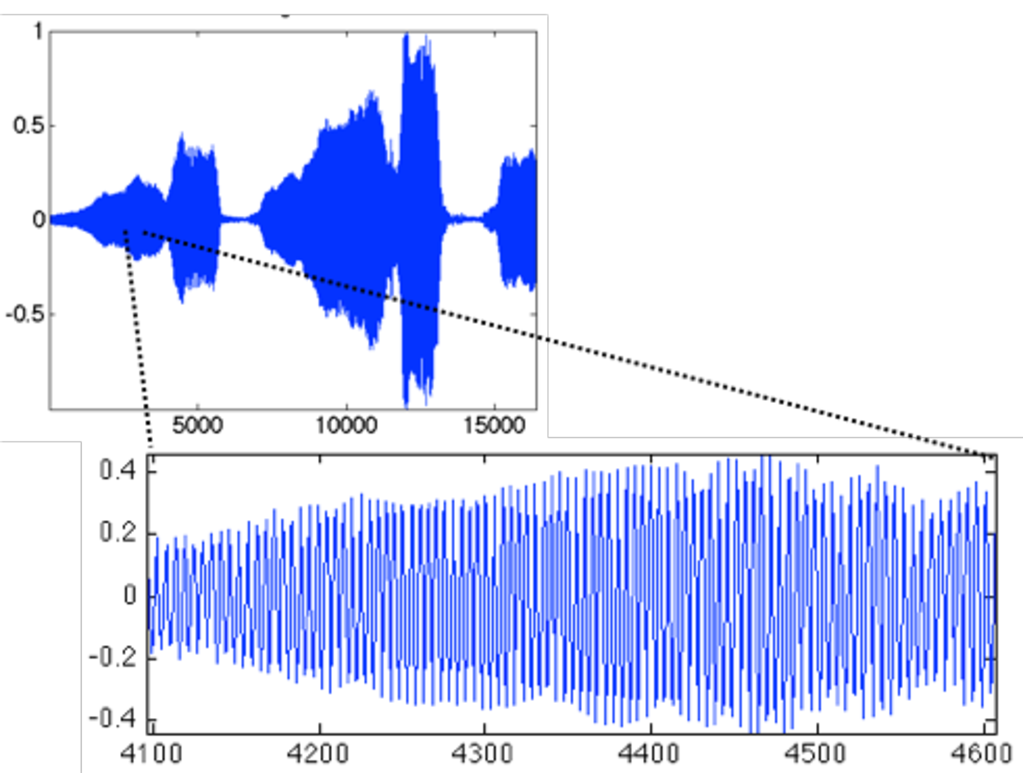
\includegraphics[width=.45\linewidth]{discrete/signal} &
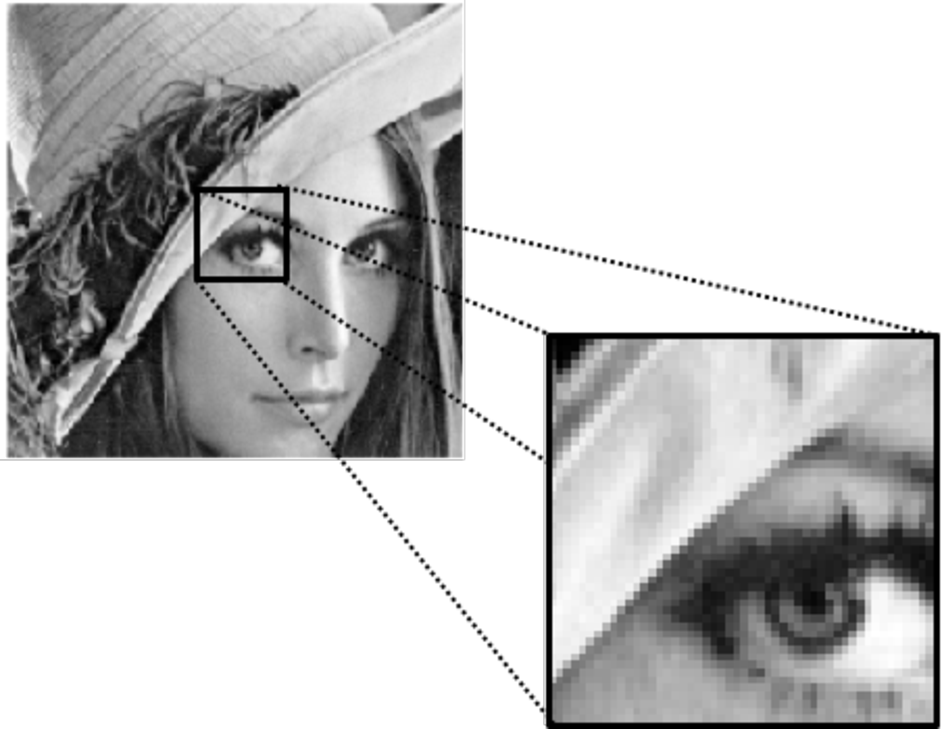
\includegraphics[width=.45\linewidth]{discrete/image}
\end{tabular}
\caption{\label{fig-samples}Exemples d'un signal sonore (donn�es 1D) et d'une image (donn�es 2D) discr�tis�s.}
\end{figure}


C'est la th�orie �labor�e par Claude Shannon~\cite{Shannon1948} qui a pos� les fondations de l'�chantillonnage (l'utilisation d'un vecteur discret $f$ afin de repr�senter fid�lement une fonction continue $\tilde f$) mais �galement celles de la compression sans perte.
%
Nous allons voir comment les recherches actuelles ont permis de b�tir sur ces fondations des m�thodes de compression avec pertes (i.e. avec un l�g�re d�gradation de la qualit�), ainsi que de revisiter l'�chantillonnage classique pour donner naissance � l'�chantillonnage compress�. 


%%%%%%%%%%%%%%%%%%%%%%%%%%%%%%%%%%%%
\section{Approximation non-lin�aire et compression}


%%%%%
\paragraph{Approximation non-lin�aire.}

La dimension $Q$ de ces donn�es est en g�n�ral tr�s grande (de l'ordre du million pour une image, du milliard pour une vid�o) et il est n�cessaire de calculer une repr�sentation plus �conome afin de pouvoir stocker $f$ ou bien le transmettre sur un r�seau. 
%
Toutes les m�thodes de compression avec perte modernes (MP3, JPEG, MPEG, etc.) utilisent pour ce faire des d�compositions parcimonieuses (c'est-�-dire compos�e de peu de coefficients non-nuls) dans un dictionnaire $\Psi = (\psi_n)_{n=1}^N$ compos� d'atomes �l�mentaires $\psi_n \in \RR^Q$.
%
On recherche ainsi � approcher $f$ � l'aide d'une combinaison lin�aire 
\eq{
	f \approx  \Psi x \eqdef \sum_{n=1}^N x_n \psi_n \in \RR^Q
}
o� les $x = (x_n)_{n=1}^N \in \RR^N$ sont les coefficients que l'on va stocker o� transmettre. Afin que cette repr�sentation soit �conome, et que le stockage prenne peu de place, il est n�cessaire qu'un maximum de coefficients $x_n$ soient nuls, de sorte que l'on n'ait � stocker que les coefficients non nuls. Etant donn� un budget $M>0$ de coefficients non-nuls, on cherche la meilleure combinaison possible afin d'approcher en norme $\ell^2$ les donn�es de d�part. On cherche ainsi � r�soudre le probl�me d'optimisation
\eql{\label{eq-pbm-approx}
	x^\star \in \uargmin{x \in \RR^N} \enscond{  \norm{f - \Psi x}_2  }{ \norm{x}_0 \leq M }
	\qouq
	\norm{f}_2^2 \eqdef \sum_{q=1}^Q |f_q|^2.
}
Ici, on a not� $\norm{x}_0 \eqdef \sharp\enscond{n}{x_n \neq 0}$ le nombre de coefficients non-nuls de $x$, qui est une mesure de comptage que l'on appelle souvent par abus de langage la \guill{pseudo-norme} $\ell^0$ (qui n'est pas une norme !). Cet abus de langage sera expliqu� � la section~\ref{sec-pb-inv}, voir en particulier la figure~\ref{fig-boules}.

Le probl�me~\eqref{eq-pbm-approx} est en g�n�ral impossible � r�soudre : c'est un probl�me de nature combinatoire, qui, sans hypoth�se suppl�mentaire sur $\Psi$, n�cessite l'exploration de toutes les combinaisons de $M$ coefficients non-nuls. Il a �t� prouv� que ce probl�me est en effet NP-difficile~\cite{Natarajan95}. 





%%%%%
\paragraph{Approximation dans une base orthonormale.}

Il y a cependant un cas de figure simple, qui est tr�s utile pour la compression : c'est le cas o� $\Psi$ est une base orthonorm�e de $\RR^Q$, c'est � dire que $Q=N$ et  
\eq{
	\dotp{\psi_n}{\psi_{n'}} = \choice{
		1 \qsiq n = n', \\
		0 \quad\text{sinon.}
	}
	\qouq
	\dotp{f}{g} \eqdef \sum_{q=1}^Q f_q g_q.
}
Ce cas est celui que l'on rencontre le plus souvent pour la compression de donn�es, et on peut citer par exemple les bases orthogonales de Fourier discr�tes, de cosinus locaux (utilis�s pour MP3, JPG et MPG) et d'ondelettes (utilis�es pour JPEG2000), voir le livre~\cite{mallat2009a-wav}. 
%
Dans ce cas, on a l'identit� de Parseval qui correspond � la d�composition de $f$ dans une base orthonorm�e
\eql{\label{eq-expansion-bon}
	f = \sum_{n=1}^N \dotp{f}{\psi_n} \psi_n 
	\qetq
	\norm{f - \Psi x}_2^2 = \sum_{n=1}^N | \dotp{f}{\psi_n} - x_n |^2.
}
Ces formules montrent que la solution de~\eqref{eq-pbm-approx} se calcule tr�s simplement. 
%
En effet, pour minimiser $\norm{f - \Psi x}_2$, pour chaque $x_n$ non-nul, il convient de choisir $x_n = \dotp{f}{\psi_n}$. 
%
Et comme on se fixe un budget maximum de $M$ coefficients non nuls, il faut choisir les $M$ plus grands coefficients $|\dotp{f}{\psi_n}|$ dans la formule~\eqref{eq-expansion-bon}. Math�matiquement, si on note $|\dotp{f}{\psi_{n_1}}| \geq |\dotp{f}{\psi_{n_2}}| \geq \ldots$ un classement des coefficients par ordre d�croissant, alors une solution $x^\star$ de~\eqref{eq-pbm-approx} est donn�e par  
\eql{\label{eq-formule-thresh}
	x^\star_n = \choice{
		\dotp{f}{\psi_{n}} \qsiq n \in \{n_1,\ldots,n_M\}, \\
		0 \quad\text{sinon.}		
	}
}

\newcommand{\myPic}[1]{\includegraphics[trim=50 50 30 30,clip,width=.24\linewidth]{approx/#1}}
\begin{figure}\centering
\begin{tabular}{@{}c@{\hspace{1mm}}c@{\hspace{1mm}}c@{\hspace{1mm}}c@{}}
\myPic{cameraman} &
\myPic{cameraman-4} &
\myPic{cameraman-8} &
\myPic{cameraman-16} \\
$f$ & 
$\Psi x^\star, M=N/4$ & 
$\Psi x^\star, M=N/8$ &  
$\Psi x^\star, M=N/16$ 
\end{tabular}
\caption{\label{fig-approx}Exemples d'approximation $f \approx \Psi x^\star$ avec $M=\norm{x^\star}_0$ qui varie, pour une image $f \in \RR^N$ de $N=256^2$ pixels. }
\end{figure}


La figure~\ref{fig-approx} montre des approximations $f \approx \Psi x^\star$ ainsi calcul�es, avec un nombre $M = \norm{x^\star}_0$ variable de coefficients.
%
Ces approximations sont r�alis�es � l'aide d'une base orthogonale d'ondelettes $\Psi$, dite base de Daubechies 4, qui sont semblables aux fonctions utilis�es dans le standard de compression d'image JPEG2000, et sont populaires car il existe un algorithme rapide pour calculer les produits scalaires $( \dotp{f}{\psi_{n}} )_n$ en un temps de calcul proportionnel � $Q$ (voir le livre~\cite[Chap. 7]{mallat2009a-wav} pour une description compl�te de la th�orie et la pratique num�rique des ondelettes). 
%
On peut voir que la qualit� de l'image reconstruite $\Psi x^\star$ se d�grade lorsque $M$ diminue, mais on peut quand m�me r�duire consid�rablement la quantit� d'information � stocker (le taux de compression $M/Q$ est petit), tout en gardant une qualit� visuelle acceptable. 
%
Cette observation fondamentale correspond au fait (observ� en pratique) que les images usuelles sont tr�s bien approch�es par une combinaison lin�aire \guill{parcimonieuse} de la forme $\Psi x^\star$ avec $\norm{x^\star}_0 \leq M$. 
%
Il est important de remarquer que, bien que le calcul de $\Psi x^\star$ � partir $x^\star$ est une formule \textit{lin�aire}, le calcul de $x^\star$ � partir de $f$ est \textit{non-lin�aire}, comme on peut le voir dans la formule~\eqref{eq-formule-thresh}. Le passage de $f$ � son approximation $\Psi x^\star$ est appel� une approximation non-lin�aire.  
%
La justification th�orique de cette observation est l'objet d'�tude de la th�orie de l'approximation non-lin�aire, qui cherche � prouver que $\norm{f-\Psi x^\star}$ d�croit rapidement lorsque $M$ augmente sous certaines hypoth�ses de r�gularit� sur $f$, par exemple si on suppose que l'image est lisse par morceaux, voir~\cite[Chap. 9]{mallat2009a-wav}.

% (maintenant bien compris math�matiquement et observ� en pratique)


Afin d'obtenir un r�el algorithme de compression, il convient ensuite d'utiliser une technique permettant de convertir les $M$ coefficients $(x_{n_1},\ldots,x_{n_2})$ en �criture binaire et �galement de stocker les indices non-nuls $(n_1,\ldots,n_M)$. Ceci se fait simplement � l'aide de techniques issues de la th�orie de l'information, en particulier les m�thodes de codage entropique, voir~\cite[Chap. 10]{mallat2009a-wav}. 
%
% Cette technique d'approximation est �galement utile pour enlever du bruit dans des images, � la suite des travaux pionniers de Donoho et Jonhstone. 

%%%%%%%%%%%%%%%%%%%%%%%%%%%%%%%%%%%%%%%%%%%%%
\section{Probl�mes inverses et parcimonie}
\label{sec-pb-inv}

%%%%%
\paragraph{Probl�mes inverses.}

Avant de pouvoir stocker des donn�es $f$, il est la plupart du temps n�cessaire d'effectuer une �tape pr�liminaire de restauration, qui consiste � am�liorer la qualit� des donn�es � partir d'observations de basse qualit�, c'est-�-dire de basse r�solution, possiblement floues, ent�ch�es d'erreurs et bruit�es. Afin de prendre en compte toute la cha�ne de formation des donn�es, on mod�lise math�matiquement le processus d'acquisition sous la forme 
\eql{\label{eq-fwd-model}
	y = \Phi f + w \in \RR^P
}
o� $y \in \RR^P$ sont les $P$ observations mesur�es par l'appareil, $w \in \RR^P$ est un bruit de mesure (inconnu), $f \in \RR^Q$ est l'image (inconnue) que l'on souhaite r�cup�rer, et $\Phi : \RR^Q \rightarrow \RR^P$ est un op�rateur mod�lisant l'appareil d'acquisition, et que l'on suppose \textit{lin�aire}. Ceci signifie que l'on peut consid�rer $\Phi$ comme �tant une (gigantesque) matrice $\Phi \in \RR^{P \times Q}$.  Il est important de noter que la plupart du temps, on ne stocke jamais explicitement cette matrice $\Phi$, elle est manipul�e de fa�on implicite � l'aide d'op�rations rapides (convolution, masquage, etc.). 


\begin{figure}\centering
\begin{tabular}{@{}c@{\hspace{4mm}}c@{\hspace{4mm}}c@{}}
\includegraphics[width=.25\linewidth]{operators/lena-original} &
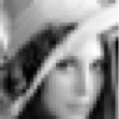
\includegraphics[width=.25\linewidth]{operators/lena-blurring} &
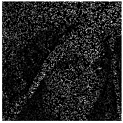
\includegraphics[width=.25\linewidth]{operators/lena-inpainting} \\
Image originale $f$ & $\Phi f$ (flou) & $\Phi f$ (masquage)  
\end{tabular}
\caption{Observations (sans bruit, $w=0$) $y=\Phi f$ dans le cas de la convolution ($\Phi f = \phi \star f$ est une convolution par un filtre passe-bas $\phi$) et des donn�es manquantes ($\Phi=\diag(\mu_q)_{q=1}^Q$ est un op�rateur de masquage).  \label{fig-exemple-ip} }
\end{figure}



Ce mod�le, qui peut para�tre assez restrictif (en particulier l'hypoth�se de lin�arit�) permet de mod�liser une quantit� surprenante de situations que l'on rencontre en pratique. On peut par exemple citer : 
\begin{itemize}
	\item le d�bruitage : $\Phi = \Id_{\RR^Q}$, $P=Q$ et on est dans la situation (la plus simple) dans laquelle on ne cherche qu'� enlever le bruit $w$ ; 
	 \item la d�convolution (voir figure~\eqref{fig-exemple-ip}, milieu) : $\Phi f = \phi \star f$ est une convolution par un filtre $\phi$ mod�lisant par exemple le flou d'un appareil photo (soit un flou de boug�, soit un flou d� � la mise au point) ; 
	 \item les donn�es manquantes (voir figure~\eqref{fig-exemple-ip}, droite) : $\Phi=\diag(\mu_q)_{q=1}^Q$ est un op�rateur de masquage diagonal, tel que $\mu_q=1$ si la donn�es index�e par $q$ (par exemple un pixel) est observ�e, et $\mu_q=0$ si la donn�e est manquante ; 
	 \item l'imagerie tomographique : $\Phi$ est un op�rateur lin�aire plus complexe, calculant des int�grales le long de lignes droites (la transform�e de Radon), voir \cite[Sect. 2.4]{mallat2009a-wav}.
\end{itemize}
Il existe quantit� d'autres exemples (en imagerie m�dicale, sismique, astrophysique, etc.), et � chaque fois, calculer une bonne approximation de $f$ � partir de $y$ est tr�s difficile. En effet, � l'exception du cas \guill{facile} du d�bruitage (i.e. $\Phi=\Id_{\RR^Q}$), on ne peut pas utiliser la formule $\Phi^{-1} y = f + \Phi^{-1} w$, soit parce que $\Phi$ n'est pas inversible (par exemple pour les donn�es manquantes), soit parce que $\Phi$ a des valeurs propres tr�s petites (pour la d�convolution ou la tomographie), de sorte que $\Phi^{-1}w$ va �tre tr�s grand, et donc $\Phi^{-1} y$ est une approximation tr�s mauvaise de $f$.


%%%%%
\paragraph{R�gularisation parcimonieuse.}

Pour rem�dier � ce probl�me, il faut remplacer $\Phi^{-1}$ par une \guill{inverse} approch�e qui prend en compte des hypoth�ses suppl�mentaires sur le signal $f$ que l'on cherche. Les m�thodes r�centes, qui donnent les meilleurs r�sultats sur des donn�es complexes, utilisent une inverse approch�e qui est non-lin�aire. Ceci peut sembler contradictoire car $\Phi$ est lin�aire, mais l'utilisation de m�thodes non-lin�aires est cruciale pour tirer parti d'hypoth�ses r�alistes sur les donn�es complexes telles que des images. 
%
En s'inspirant des techniques d'approximation et de compression discut�es dans la section pr�c�dente, les m�thodes actuelles cherchent � exploiter le fait que l'on peut bien approcher $f$ � l'aide d'une approximation parcimonieuse $\Psi x$ avec $\norm{x}_0 \leq M$. Etant donn� un param�tre $M>0$, on va chercher � approcher $f$ par $f^\star = \Psi x^\star$ o� $x^\star$ est une solution de 
\eql{\label{eq-pbm-l0}
	x^\star \in \uargmin{x \in \RR^N} \enscond{  \norm{y - \Phi \Psi x}_2  }{ \norm{x}_0 \leq M }
}
On voit que~\eqref{eq-pbm-l0} est quasi-identique �~\eqref{eq-pbm-approx}, sauf que l'on a remplac� $f \in \RR^Q$ (que l'on ne conna�t pas) par $y\in \RR^P$, et que l'on a remplac� la matrice $\Psi \in \RR^{Q \times N}$ par le produit matriciel $\Phi \Psi \in \RR^{P \times N}$. Dans le cas particulier du d�bruitage, $\Phi=\Id_{\RR^Q}$, les probl�mes~\eqref{eq-expansion-bon} et~\eqref{eq-pbm-l0} sont �quivalents et ont la m�me solution, de sorte que l'approximation non-lin�aire permet de r�soudre le probl�me de d�bruitage.

Dans le cas d'un op�rateur $\Phi$ quelconque, le probl�me~\eqref{eq-pbm-l0} est cependant un probl�me d'optimisation extr�mement difficile � r�soudre. En effet, m�me si $\Psi$ est une base orthonorm�e, en g�n�ral (sauf dans le cas du d�bruitage $\Phi=\Id_{\RR^Q}$), la matrice $\Phi \Psi$ n'est pas orthogonale, de sorte que la formule~\eqref{eq-formule-thresh} n'est pas applicable, et~\eqref{eq-pbm-l0} est un probl�me de recherche combinatoire NP-difficile.


%%%%%
\paragraph{R�gularisation $\ell^1$.}

L'approximation des solutions du probl�me~\eqref{eq-pbm-l0} � l'aide de m�thodes efficaces est un des sujets de recherche les plus actifs en traitement de donn�es (et plus g�n�ralement en math�matiques appliqu�es, imagerie, statistique et apprentissage) de ces vingt derni�res ann�es. Il existe de nombreuses m�thodes, parmi lesquelles les algorithmes gloutons (voir par exemple~\cite{MallatMP}) et les m�thodes par relaxation convexe. Nous allons nous attarder principalement sur cette deuxi�me classe de m�thodes. 
%
Une fa�on (heuristique) d'introduire ces techniques consiste � remplacer $\norm{\cdot}_0$ dans le probl�me~\eqref{eq-pbm-l0} par la fonction~${\norm{\cdot}_\al^\al}$, qui est d�finie, pour $\al>0$, par
\eq{
	\norm{x}_{\al}^\al \eqdef \sum_{n=1}^N |x_n|^\al.
}
La figure~\ref{fig-boules} montre dans le cas (irr�aliste, mais bien pratique pour faire un dessin) de $N=2$ coefficients, les boules unit�s $B_\al \eqdef \enscond{x}{\norm{x}_\al \leq 1}$ associ�es � ces fonctionnelles $\norm{\cdot}_\al$. On peut ainsi voir que $B_\al$ \guill{tend} vers la \guill{boule} unit� associ�e � la mesure de comptage $\norm{\cdot}_0$ � mesure que $\al$ tend vers $0$, c'est-�-dire que
\eq{
	B_\al \overset{\al \rightarrow 0}{\longrightarrow} B_0 \eqdef \enscond{ x \in [-1,1]^N }{ \norm{x}_0 \leq 1 },
}
la convergence de ces ensembles (que l'on visualise bien sur la figure) �tant au sens par exemple de la distance de Hausdorff. 
%
La boule limite $B_0$ est constitu�e de vecteurs extr�mement parcimonieux, puisqu'ils sont compos�s d'une seule composante non-nulle.



\begin{figure}\centering
\begin{tabular}{@{}c@{\hspace{1mm}}c@{\hspace{1mm}}c@{\hspace{1mm}}c@{\hspace{1mm}}c@{}}
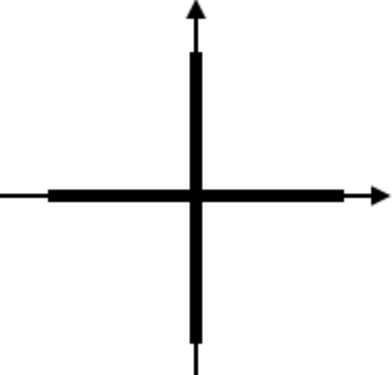
\includegraphics[width=.19\linewidth]{balls/l0} &
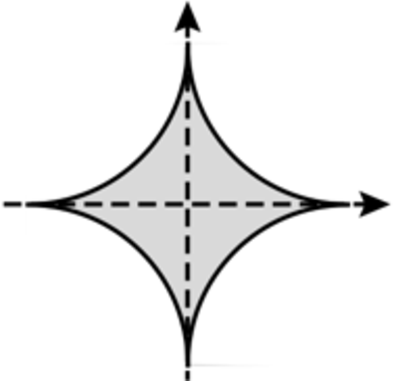
\includegraphics[width=.19\linewidth]{balls/l12} &
\includegraphics[width=.19\linewidth]{balls/l1} &
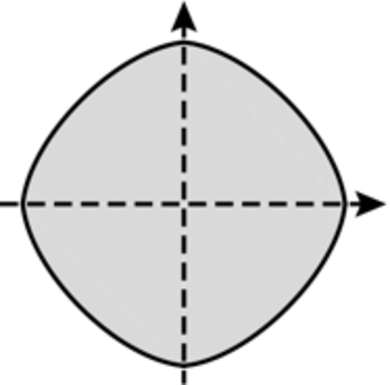
\includegraphics[width=.19\linewidth]{balls/l32} &
\includegraphics[width=.19\linewidth]{balls/l2} \\
$\al=0$ & $\al=1/2$ & $\al=1$ & $\al=3/2$ & $\al=2$
\end{tabular}
\caption{\label{fig-boules}Boules $B_\al$ pour diff�rentes valeurs de $\al$. }
\end{figure}


On est alors amen� � prendre en compte deux �l�ments contradictoires pour choisir une valeur de $\al$ :
\begin{itemize}
	\item Afin d'avoir une fonctionnelle privil�giant au maximum les vecteurs parcimonieux, on souhaite utiliser une valeur de $\al$ la plus faible possible pour remplacer $\norm{\cdot}_0$ par $\norm{\cdot}_\al$. 
	\item Afin de pouvoir calculer la solution de~\eqref{eq-pbm-l0} avec $\norm{\cdot}_\al$ � la place de $\norm{\cdot}_0$, il est important que la fonctionnelle $\norm{\cdot}_\al$ soit \textit{convexe}. La convexit� est en effet essentielle afin d'obtenir un probl�me qui ne soit pas NP-difficile et pouvoir b�n�ficier d'algorithmes rapides de calcul. Ces algorithmes trouvent une solution exacte $x^\star$ en temps polynomial ou bien convergent rapidement vers cette solution.
\end{itemize}
La contrainte de convexit� de $\norm{\cdot}_\al$ impose que l'ensemble $B_\al$ soit convexe, ce qui, de fa�on �quivalente, signifie que $\norm{\cdot}_\al$ doit �tre une \textit{norme}. Ceci impose que $\al \geq 1$. La prise en compte de ces deux contraintes m�ne ainsi naturellement au choix \guill{optimal} $\al=1$, de sorte que l'on va consid�rer le probl�me d'optimisation convexe (c'est-�-dire que l'on cherche � minimiser une fonction convexe sur un ensemble convexe)
\eql{\label{eq-pbm-l1}
	x^\star \in \uargmin{x \in \RR^N} \enscond{  \norm{y - \Phi \Psi x}_2  }{ \norm{x}_1 = \sum_{n=1}^N |x_n| \leq \tau }, 
}
de sorte que l'image calcul�e comme solution est $f^\star = \Psi x^\star$.
%
On peut noter que l'on a utilis� ici un param�tre $\tau > 0$ qui joue un r�le similaire au param�tre $M$ qui appara�t dans~\eqref{eq-pbm-l0}.
%
La question du choix de ce param�tre $\tau$ est cruciale. Si le bruit $w$ est petit, alors on souhaite que $\Phi f^\star = \Phi\Psi x^\star$ soit proche de $y$, et donc on va choisir $\tau$ grand. Au contraire, si le bruit $w$ est important, afin d'obtenir un effet de d�bruitage plus important, on va r�duire la valeur de $\tau$. Le choix d'un $\tau$ \guill{optimal} est un probl�me de recherche difficile, et il n'existe pas de r�ponse \guill{universelle}, les strat�gies existantes d�pendent fortement de l'op�rateur $\Phi$ ainsi que de la famille d'atomes~$\Psi$.

Le probl�me~\eqref{eq-pbm-l1} a initialement �t� propos� par des ing�nieurs dans les domaines de l'imagerie sismique (voir par exemple~\cite{santosa1986linear}), et il a �t� introduit conjointement en traitement du signal sous le nom \guill{basis pursuit}~\cite{chen1999atomi} et en statistique sous le nom \guill{Lasso}~\cite{tibshirani1996regre}. 


\begin{figure}\centering
\begin{tabular}{@{}c@{\hspace{4mm}}c@{\hspace{4mm}}c@{}}
\includegraphics[width=.25\linewidth]{inpainting/lena-original}&
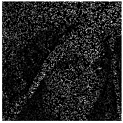
\includegraphics[width=.25\linewidth]{inpainting/lena-observations}&
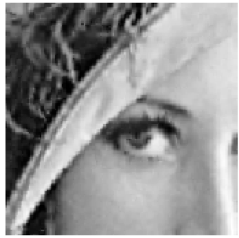
\includegraphics[width=.25\linewidth]{inpainting/lena-reconstructed}\\
$f$ original & Observations $y$ & Reconstruction $f^\star$
\end{tabular}
\caption{Exemples de reconstruction avec donn�es manquantes, $\Phi=\diag(\mu_q)_{q=1}^Q$ avec $\mu_q \in \{0,1\}$ et un nombre de donn�es observ�es $\sharp\enscond{q}{\mu_q=1}/Q = 10\%$.  \label{fig-inpainting} }
\end{figure}

Le probl�me~\eqref{eq-pbm-l1}, bien que convexe, reste un probl�me difficile � r�soudre � cause de la non-diff�rentiabilit� de la norme ${\norm{\cdot}_1}$ et de la grande taille des donn�es ($N$ est tr�s grand). C'est le prix � payer pour obtenir des r�sultats de bonne qualit�. Comme nous allons l'expliquer dans le paragraphe qui suit, c'est en effet la non-diff�rentiabilit� de ${\norm{\cdot}_1}$ qui permet d'obtenir de la parcimonie. Le d�veloppement d'algorithmes efficaces pour r�soudre~\eqref{eq-pbm-l1} est un domaine de recherche tr�s actif, et nous renvoyons �~\cite[section 6]{2014-vaiter-ps-review} pour un tour d'horizon de ces m�thodes. La figure~\ref{fig-inpainting} montre un exemple d'interpolation de donn�es manquantes r�alis�e en r�solvant~\eqref{eq-pbm-l1} dans une famille $\Psi$ d'ondelettes invariantes par translation.


%%%%
\paragraph{De l'intuition � l'analyse th�orique des performances.}


La figure~\ref{fig-l1-vs-l2} montre intuitivement pourquoi la solution $x^\star$ calcul�e en rempla�ant $\norm{\cdot}_0$ par $\norm{\cdot}_\al$ dans~\eqref{eq-pbm-l0} est meilleure (au sens qu'elle est plus parcimonieuse) si on choisit $\al=1$ (c'est-�-dire si on r�sout~\eqref{eq-pbm-l1}) que si on choisit $\al=2$ (une conclusion similaire est obtenue pour d'autres valeurs de $\al>1$). 
% 
La figure est fait dans le cas (tr�s simple) de $N=2$ coefficients et $P=1$ observations. Le point crucial, qui rend la solution de~\eqref{eq-pbm-l1} parcimonieuse, est que la boule $B_1$ associ�e � la norme $\ell^1$ est \guill{pointue} de sorte que la solution $x^\star$ est situ�e le long des axes. Ceci n'est pas le cas pour la boule $B_2$ associ�e � la norme $\ell^2$, qui donne une solution $x^\star$ qui n'est pas le long des axes, et n'est donc pas parcimonieuse.
%
Ce ph�nom�ne, d�j� visible en dimension 2, est en fait accentu� lorsque la dimension augmente, de sorte que l'approximation obtenue en rempla�ant $\norm{\cdot}_0$ par $\norm{\cdot}_1$ devient meilleure en grande dimension. 
% 
Ce ph�nom�ne est appel� par David Donoho la \guill{b�n�diction de la grand dimension}~\cite{DonohoCurse} : bien que les donn�es deviennent tr�s co�teuses et complexes � traiter (la \guill{mal�diction de la dimension}) on dispose de techniques efficaces pour les analyser si elles sont suffisamment parcimonieuses. 
%
Rendre cette intuition rigoureuse est cependant difficile, et c'est l'objet de recherches encore en cours pour des op�rateurs $\Phi$ tels que des convolutions~\cite{candes-towards2013,2015-duval-focm}. L'analyse dans le cas des op�rateurs que l'on rencontre par exemple en imagerie m�dicale est un probl�me math�matique ouvert.


\begin{figure}\centering
\begin{tabular}{@{}c@{\hspace{4mm}}c@{}}
\includegraphics[width=.35\linewidth]{l1-vs-l2/l1} &
\includegraphics[width=.35\linewidth]{l1-vs-l2/l2} \\
Minimisation $\ell^1$ & Minimisation $\ell^2$
\end{tabular}
\caption{Comparaison de la minimisation avec des contraintes de type $\norm{x}_\al \leq \tau$  pour $\al�\in \{1,2\}$.
%
Une solution $x^\star$ est obtenue lorsque l'on trouve un tube $\enscond{x}{\norm{\Phi x-y} \leq \epsilon}$ assez grand (i.e. en faisant croitre progressivement $\epsilon$) tel qu'il soit tangent en $x^\star$ � la boule $\enscond{x}{\norm{x}_\al \leq \tau}$.  \label{fig-l1-vs-l2} }
\end{figure}



%%%%%%%%%%%%%%%%%%%%%%%%%%%%%%%%%%%%%%%%%%%%%
\section{L'�chantillonnage compress�}

Il existe une classe particuli�re d'op�rateurs $\Phi$ pour laquelle il est possible d'analyser tr�s pr�cis�ment les performances obtenues lorsque l'on r�sout~\eqref{eq-pbm-l1}. Il s'agit du cas o� $\Phi$ est tir� al�atoirement selon certaines distributions de matrices al�atoires. Utiliser des matrices al�atoires peut sembler �trange, car les op�rateurs mentionn�s plus haut (convolution,  tomographie, etc.) ne le sont pas du tout. 
%
En fait, ce choix est motiv� par une application concr�te propos�e conjointement par Cand�s, Tao et Romberg~\cite{candes2006stable} ainsi que Donoho~\cite{donoho2006compressed}, et que l'on appelle commun�ment \guill{�chantillonnage compress�} (\guill{compressed sensing} en anglais). 



%%%%
\paragraph{Appareil photo \guill{pixel unique}.}

Afin de rendre l'explication plus parlante, nous allons aborder le prototype d'appareil photo \guill{pixel unique} (\guill{single pixel cam�ra} en anglais) d�velopp� � Rice University~\cite{DuarteSinglePixel}, et qui est illustr� par la figure~\ref{fig-single-pixel} (gauche). 
%
Il s'agit de d�velopper une nouvelle classe d'appareils photos permettant de r�aliser � la fois \textit{l'�chantillonnage} et la \textit{compression} d'une image. Au lieu de d'abord �chantillonner tr�s finement (i.e. avec $Q$ tr�s grand) le signal analogique $\tilde f$ pour obtenir une image $f \in \RR^Q$ puis de compresser �norm�ment (i.e. avec $M$ petit)  en utilisant~\eqref{eq-formule-thresh}, on aimerait disposer directement d'une repr�sentation �conomique $y \in \RR^P$ de l'image, avec un budget $P$ aussi proche de $M$ et tel que l'on soit capable de \guill{d�compresser} $y$ pour obtenir une bonne approximation de l'image $f$.

L'appareil \guill{pixel unique} permet de r�aliser l'�chantillonnage compress� d'une sc�ne observ�e $\tilde f$ (la lettre \guill{R}�sur la Figure~\ref{fig-single-pixel}), qui est une fonction continue indiquant la quantit� de lumi�re $\tilde f(s)$ atteignant chaque point $s \in \RR^2$ du plan focal de la camera. 
%
Pour ce faire, la lumi�re est focalis�e contre un jeu de $Q$ micro-miroirs tapissant le plan focal. Ces micro-miroirs ne sont pas des capteurs. Contrairement � l'�chantillonnage classique (d�crit � la section~\ref{sec-echantillonnage}), ils n'enregistrent aucune information, mais ils peuvent chacun �tre positionn� pour refl�ter ou absorber la lumi�re. 
%
Pour r�aliser l'enregistrement complet, on change tr�s rapidement $P$ fois les configurations des micro-miroirs. Pour $p=1,\ldots,P$, on note ainsi $\Phi_{p,q} \in \{0,1\}$ suivant que le micro-miroir � la position $q$ a �t� mis en position absorbante (valeur 0) ou r�fl�chissante (valeur 1) � l'�tape $p$ de l'acquisition. 
%
La lumi�re totale r�fl�chie � l'�tape $p$ est ensuite accumul�e en un capteur unique (d'o� le nom de \guill{pixel unique}, en fait il s'agit plut�t d'un \guill{capteur unique}), not� \guill{PD} sur la figure, ce qui r�alise une somme lin�aire des intensit�s r�fl�chies pour obtenir la valeur $y_p \in \RR$ enregistr�e. 
%
Au final, si l'on note (comme  � la section~\ref{sec-echantillonnage}) $f_q = \int_{c_q} \tilde f(s) \text{d} s$ l'intensit� de lumi�re qui arrive sur la surface $c_q$ du miroir index� par $q$, l'�quation qui relie l'image discr�te $f \in \RR^Q$ \guill{vue par les miroirs}�aux $P$ mesures $y \in \RR^P$ est 
\eq{
	\foralls p = 1,\ldots,P, \quad
	y_p = \sum_q \Phi_{p,n} \int_{c_n} \tilde f(s) \text{d} s = (\Phi f)_p, 
}
ce qui correspond exactement �~\eqref{eq-fwd-model}.
%
Il est important de noter que les miroirs n'enregistrent rien, donc en particulier, l'image discr�te $f$ n'est jamais calcul�e ou enregistr�e, l'appareil calculant directement la repr�sentation compress�e $y$ depuis le signal analogique $\tilde f$. 
%
Le terme $w$ mod�lise ici les imperfections d'acquisition (bruit de mesure). L'�chantillonnage compress� correspond donc au passage de la sc�ne observ�e $\tilde f$ au vecteur directement compress� $y$. La \guill{d�compression} correspond � la r�solution d'un probl�me inverse, qui a pour but de retrouver une bonne approximation de $f$ (l'image discr�te \guill{id�ale} telle que vue par les micro-miroirs) � partir de $y$.


\begin{figure}\centering
\begin{tabular}{@{}c@{\hspace{1mm}}c@{\hspace{1mm}}c@{}}
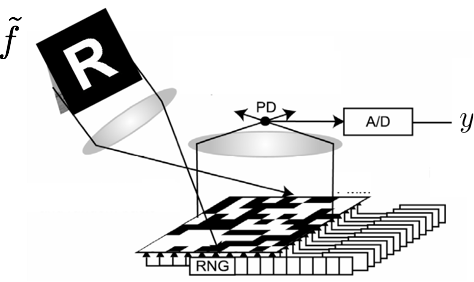
\includegraphics[width=.45\linewidth]{single-pixel/single-pixel-schema}&

\includegraphics[width=.25\linewidth]{single-pixel/reconstruction-1}&

\includegraphics[width=.25\linewidth]{single-pixel/reconstruction-6}\\
Sch�ma de l'appareil & $f$ &  $f^\star$, $P/Q=6$
\end{tabular}
\caption{Gauche : sch�ma de la m�thode d'acquisition par pixel unique.
%
Centre : image $f \in \RR^Q$ \guill{id�ale} observ�e dans le plan focal des micro-miroirs. 
% 
Droite : image $f^\star=\Psi x^\star$ reconstruite � partir d'observation $y \in \RR^P$ avec un facteur de compression $P/Q=6$.
\label{fig-single-pixel} }
\end{figure}




%%%%
\paragraph{Garanties th�oriques.}

Une particularit� importante de ce probl�me inverse est que l'on peut choisir comme on le souhaite les configurations des micro-miroirs, ce qui revient � dire que l'on peut choisir librement la matrice $\Phi \in \{0,1\}^{P \times Q}$. La question est donc de faire le meilleur choix, de sorte que l'on puisse r�soudre efficacement le probl�me inverse. Si l'on fait l'hypoth�se que le signal $f$ � reconstruire est compressible dans une base orthonorm�e $\Psi$ (c'est-�-dire que $f \approx \Psi x_0$ avec $M \eqdef \norm{x_0}_0$ petit), alors de nombreux travaux, � commencer par~\cite{candes2006stable,donoho2006compressed}, ont montr� que la m�thode~\eqref{eq-pbm-l1} �tait efficace si l'on choisit $\Phi$ comme une r�alisation de certaines matrices al�atoires. Pour le cas de l'appareil photo � pixel unique, on peut ainsi tirer chaque $\Phi_{p,n}$ al�atoirement avec une probabilit� de $1/2$ pour les valeurs $0$ et $1$. 
%
En pratique, on utilise un g�n�rateur pseudo-al�atoire, de sorte qu'� la fois la personne qui compresse les donn�es et la personne qui va les d�compresser conna�ssent parfaitement la matrice $\Phi$ (car elles peuvent se communiquer la graine du g�n�rateur). 
%
La figure~\ref{fig-single-pixel} (droite) montre un exemple de reconstruction obtenue pour le cas de l'appareil �  pixel unique avec un tel choix al�atoire de matrice $\Phi$, avec pour dictionnaire $\Psi$ une famille d'ondelettes invariantes par translation (voir~\cite[Sect. 5.2]{mallat2009a-wav} pour une description de cette famille).

Il a ainsi �t� montr� par~\cite{candes2006stable,donoho2006compressed} qu'il existe une constante $C$ telle que si l'on note $f = \Psi x_0$ o� $x_0$ sont les coefficients de l'image � retrouver, o� $\Psi$ est une base orthogonale (donc en particulier $Q=N$), et si le nombre $P$ de mesures v�rifie
\eql{\label{eq-cs-contrainte}
	\frac{P}{M} \geq C  \log\pa{\frac{N}{M}} \qouq M \eqdef \norm{x_0}_0
}
alors une solution $f^\star =\Psi x^\star$ calcul�e par~\eqref{eq-pbm-l1} tend vers $f$ lorsque le bruit $w$ tend vers $0$ et $\tau$ tend vers $+\infty$. Ce r�sultat est vrai \guill{avec forte probabilit�} sur le tirage al�atoire de la matrice $\Phi$, c'est-�-dire une probabilit� tendant rapidement vers 1 lorsque $N$ augmente. En particulier, s'il n'y a pas de bruit, $w=0$, en prenant $\tau \rightarrow +\infty$, la m�thode permet de retrouver exactement $f$ si $P$ v�rifie~\eqref{eq-cs-contrainte}. 
%
Cette th�orie permet aussi de prendre en compte des donn�es \guill{compressibles}, c'est � dire si l'on suppose uniquement que $f$ est proche de (mais pas n�cessairement �gal �) $\Psi x_0$ avec $M \eqdef \norm{x_0}_0$ petit.


De fa�on intuitive, ce r�sultat th�orique signifie que l'�chantillonnage compress� arrive � faire quasiment \guill{aussi bien} en calculant $\Psi x^\star$ � partir de $y$ (en r�solvant~\eqref{eq-pbm-l1}) qu'une m�thode de compression usuelle (MP3, JPEG, JPEG2000, MPEG, etc.) qui connaitrait exactement le signal $f$ et calculerait la meilleure approximation $\Psi x_0$ avec $M \eqdef \norm{x_0}_0$ coefficients (en r�solvant~\eqref{eq-pbm-approx} via la formule~\eqref{eq-expansion-bon}). 
%
La signification pr�cise du qualificatif \guill{aussi bien} correspond au  facteur multiplicatif $C  \log(N/M)$, qui borne $P/M$. Ce facteur correspond au \guill{surco�t} de la m�thode d'�chantillonnage compress� (qui calcule $P$ mesures) par rapport � une m�thode de compression usuelle (qui calcule $M$ coefficients). 
%
Malgr� ce surco�t, la m�thode de l'�chantillonnage compress� pr�sente de nombreux avantages : gain de temps et d'�nergie (on fait en m�me temps l'�chantillonnage et la compression), codage \guill{d�mocratique} (tous les coefficients $y_n$ jouent le m�me r�le, et donc aucun n'a de r�le pr�pond�rant, contrairement au codage des coefficients de $x_0$ qui ont une importance proportionnelle � leur amplitude), codage automatiquement crypt� (si on ne conna�t pas $\Phi$, on ne peut pas retrouver $f$ � partir de $y$). La valeur de la constante $C$ d�pend du sens que l'on donne au terme \guill{avec forte probabilit�}. Si cette probabilit� porte uniquement sur $\Phi$, mais doit �tre vraie pour tous les $x_0$ (analyse au pire cas), alors elle est tr�s grande (voir~\cite{dossal-laa-09}). Si par contre on veut qu'elle porte � la fois sur $\Phi$ et sur $x_0$ (pour que le r�sultat th�orique soit vrai pour presque tous les signaux) alors on peut montrer que par exemple, pour $N/P=4$ (compression d'un facteur $4$), on a $C  \log(N/M) \sim 4$ (voir~\cite{chandrasekaran2012convex}), ce qui reste un surco�t cons�quent, mais qui est acceptable pour certaines applications.

L'appareil photo \guill{pixel unique} est une d�clinaison particuli�re de la technique d'�chantillonnage compress�.  Les applications � la photographie sont limit�es, car les capteurs CCD des appareils photos sont performants et peu chers. L'�chantillonnage compress� aura probablement un impact pour des applications o� les mesures sont difficiles � acqu�rir ou co�tent chers. Une autre source d'applications potentielles est l'imagerie m�dicale, par exemple par r�sonance magn�tique. Dans ces domaines, il est cependant impossible d'obtenir des matrices totalement al�atoires, de sorte que l'on ne peut pas appliquer directement la th�orie de l'�chantillonnage compress�. Des r�sultats encourageants sur ces applications ont cependant �t� obtenus, voir par exemple~\cite{AdcockBreaking,Chauffert14}. 


%%%%%%%%%%%%%%%%%%%%%%%%%%%%%%%%%%%%%%%%%%%%%
\section{Conclusion}

Les avanc�es r�centes de l'analyse de donn�es ont permis d'�tendre le champ d'application de la compression afin de traiter des probl�mes inverses difficiles en imagerie, mais aussi dans d'autres domaines (syt�me de recommandation, analyse de r�seaux, etc.). Ces avanc�es ont �t� rendues possibles par l'utilisation d'un spectre tr�s large de techniques en math�matiques appliqu�es, qui couvre � la fois l'analyse harmonique, l'approximation non-lin�aire, l'optimisation non-lisse et les probabilit�s, mais �galement l'analyse fonctionnelle et les EDPs (qui n'ont pas �t� mentionn�es dans cet article). Les m�thodes parcimonieuses associ�es � la r�gularisation $\ell^1$ ne sont pourtant que la partie �merg�e de l'iceberg, et des r�gularisations plus fines permettent d'obtenir de meilleurs r�sultats en prenant en compte les structures g�om�triques complexes des donn�es. Pour plus de d�tails sur ces derni�res avanc�es, nous recommandons la lecture de l'article~\cite{2014-vaiter-ps-review}, ainsi que la visite du site web \guill{Numerical Tours of Signal Processing}~\cite{2011-peyre-cise}, qui pr�sente de nombreux codes informatiques pour r�aliser les exp�riences num�riques pr�sent�es ici, ainsi que de nombreuses autres. 

%%%%%%%%%%%%%%%%%%%%%%%%%%%%%%%%%%%%%%%%%%%%%
\paragraph{Remerciements}

Je tiens � remercier Charles Dossal, Jalal Fadili, Samuel Vaiter, St�phane Seuret et le relecteur anonyme pour leur aide pr�cieuse. 



% !TEX root = ../TransportFR.tex


\newcommand{\Blu}[1]{{\color{blue}#1}}
\newcommand{\Red}[1]{{\color{red}#1}}
\newcommand{\iC}{\Red{i}}
\newcommand{\jC}{\Blu{j}}
\newcommand{\aC}{\Red{a}}
\newcommand{\bC}{\Blu{b}}


\ifdefined\otarticle
\newcommand{\myparagraph}[1]{\subsection{#1}}
\else
\newcommand{\myparagraph}[1]{\paragraph{#1}}
\chapter{Le transport optimal numérique et ses applications}
\fi

\label{chap-ot}


%%%%%%%%%%%%%%%%%%%%%%%%%%%%%%%%%%%%%%%%%%%%%%
\section{Le Transport Optimal de Monge}

Gaspard Monge, en plus d'être un grand mathématicien, a participé activement à la révolution Française, et a créé l'\'Ecole Polytechnique ainsi que l'\'Ecole Normale Supérieure. Motivé par des applications militaires, il a formulé en 1781 le problème du transport optimal~\cite{Monge1781}~: il s'est posé la question du calcul de la façon la plus économique de transporter de la terre entre deux endroits pour faire des remblais. Dans son texte original, il a fait l'hypothèse que le coût du déplacement d'une unité de masse est égal à la distance parcourue, mais on peut utiliser n'importe quel coût adapté au problème à résoudre. 

%%%%%%%%%%%%%%%%%%%%%%%%%%%%%%%%%%%%%%%%%%%%%%%%%%%%%
\myparagraph{Le problème de Monge}

Pour illustrer le problème et sa formulation mathématique, intéressons-nous à la façon optimale de distribuer les croissants depuis les boulangeries vers les cafés, le matin dans Paris. Pour simplifier, nous allons supposer qu'il y a uniquement six boulangeries et cafés, que l'on peut voir à la figure~\ref{fig:image-cafe} (les boulangeries sont en \Red{rouge} et les cafés en \Blu{bleu}). 
%
On suppose que toutes les boulangeries produisent le même nombre de croissants et que tous les cafés demandent également ce même nombre de croissant.
%
Le coût à minimiser est le temps total des trajets, et l'on note $C_{\iC,\jC}$ le temps entre la boulangerie $\iC \in \{1,\ldots,6\}$  et le café $\jC \in \{1,\ldots,6\}$. Par exemple, on a $C_{\Red{3},\Blu{4}}=10$, ce qui signifie qu'il y a dix minutes de trajet entre la boulangerie numéro $\Red{3}$ et le café numéro $\Blu{4}$. 

\begin{figure}\centering
    \begin{tabular}{@{}c@{\hspace{1mm}}c@{\hspace{4mm}}c@{\hspace{1mm}}c@{}}
        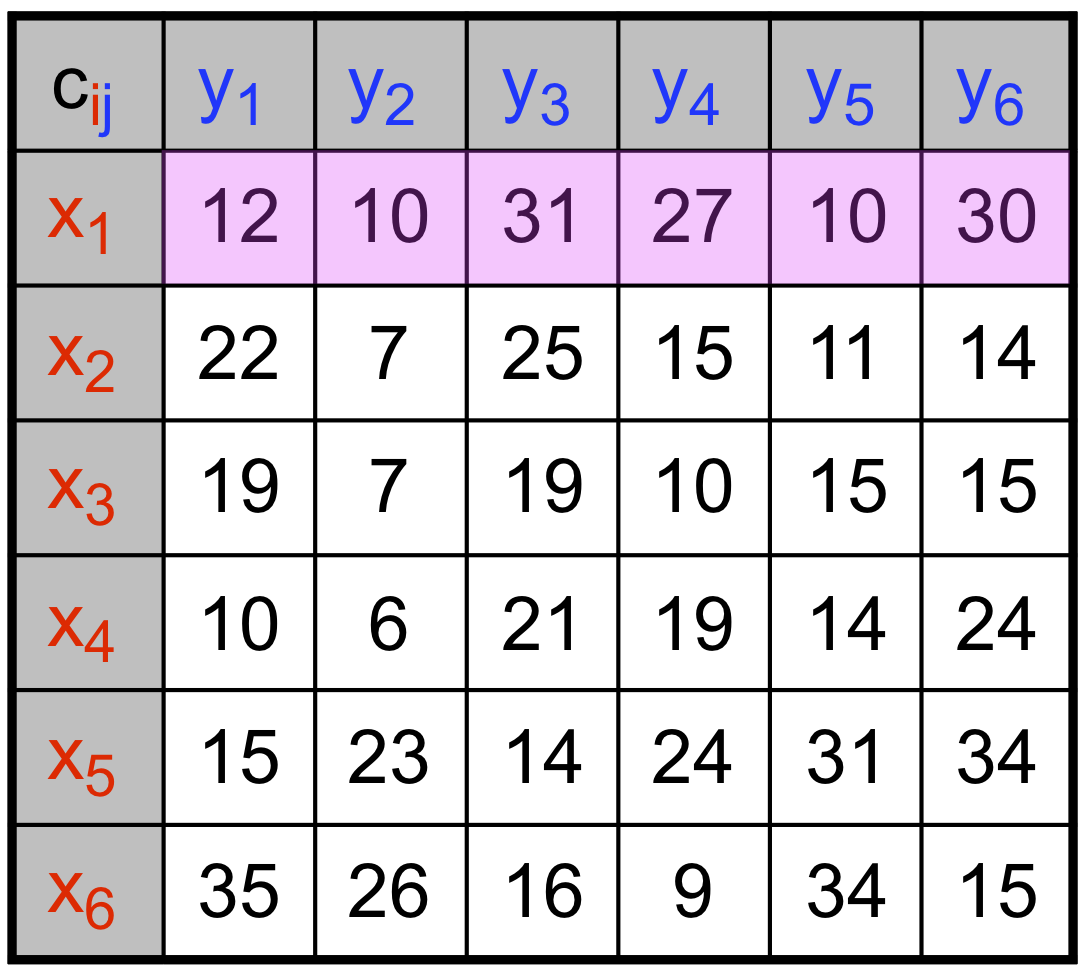
\includegraphics[width=.22\linewidth]{transport/cafe-paris/map-paris-0-couts} 
        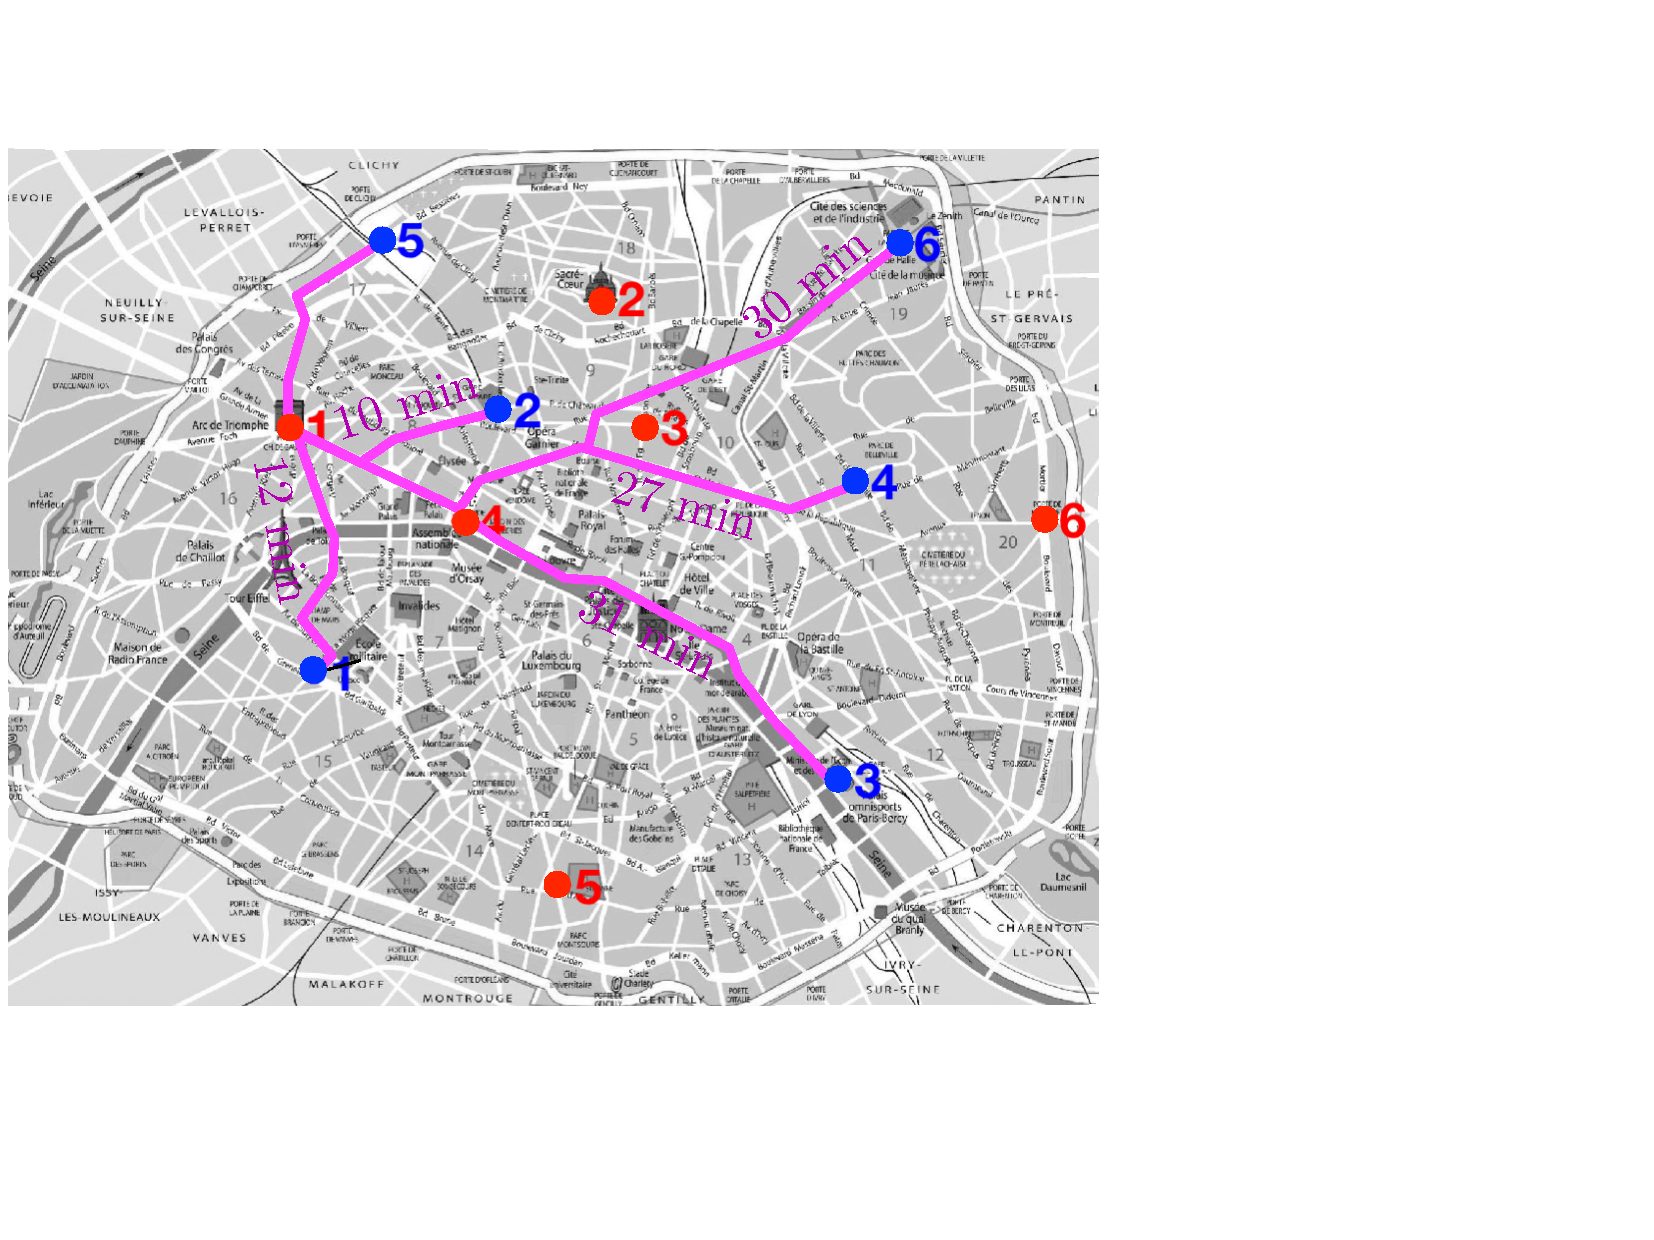
\includegraphics[width=.27\linewidth]{transport/cafe-paris/map-paris-0} 
        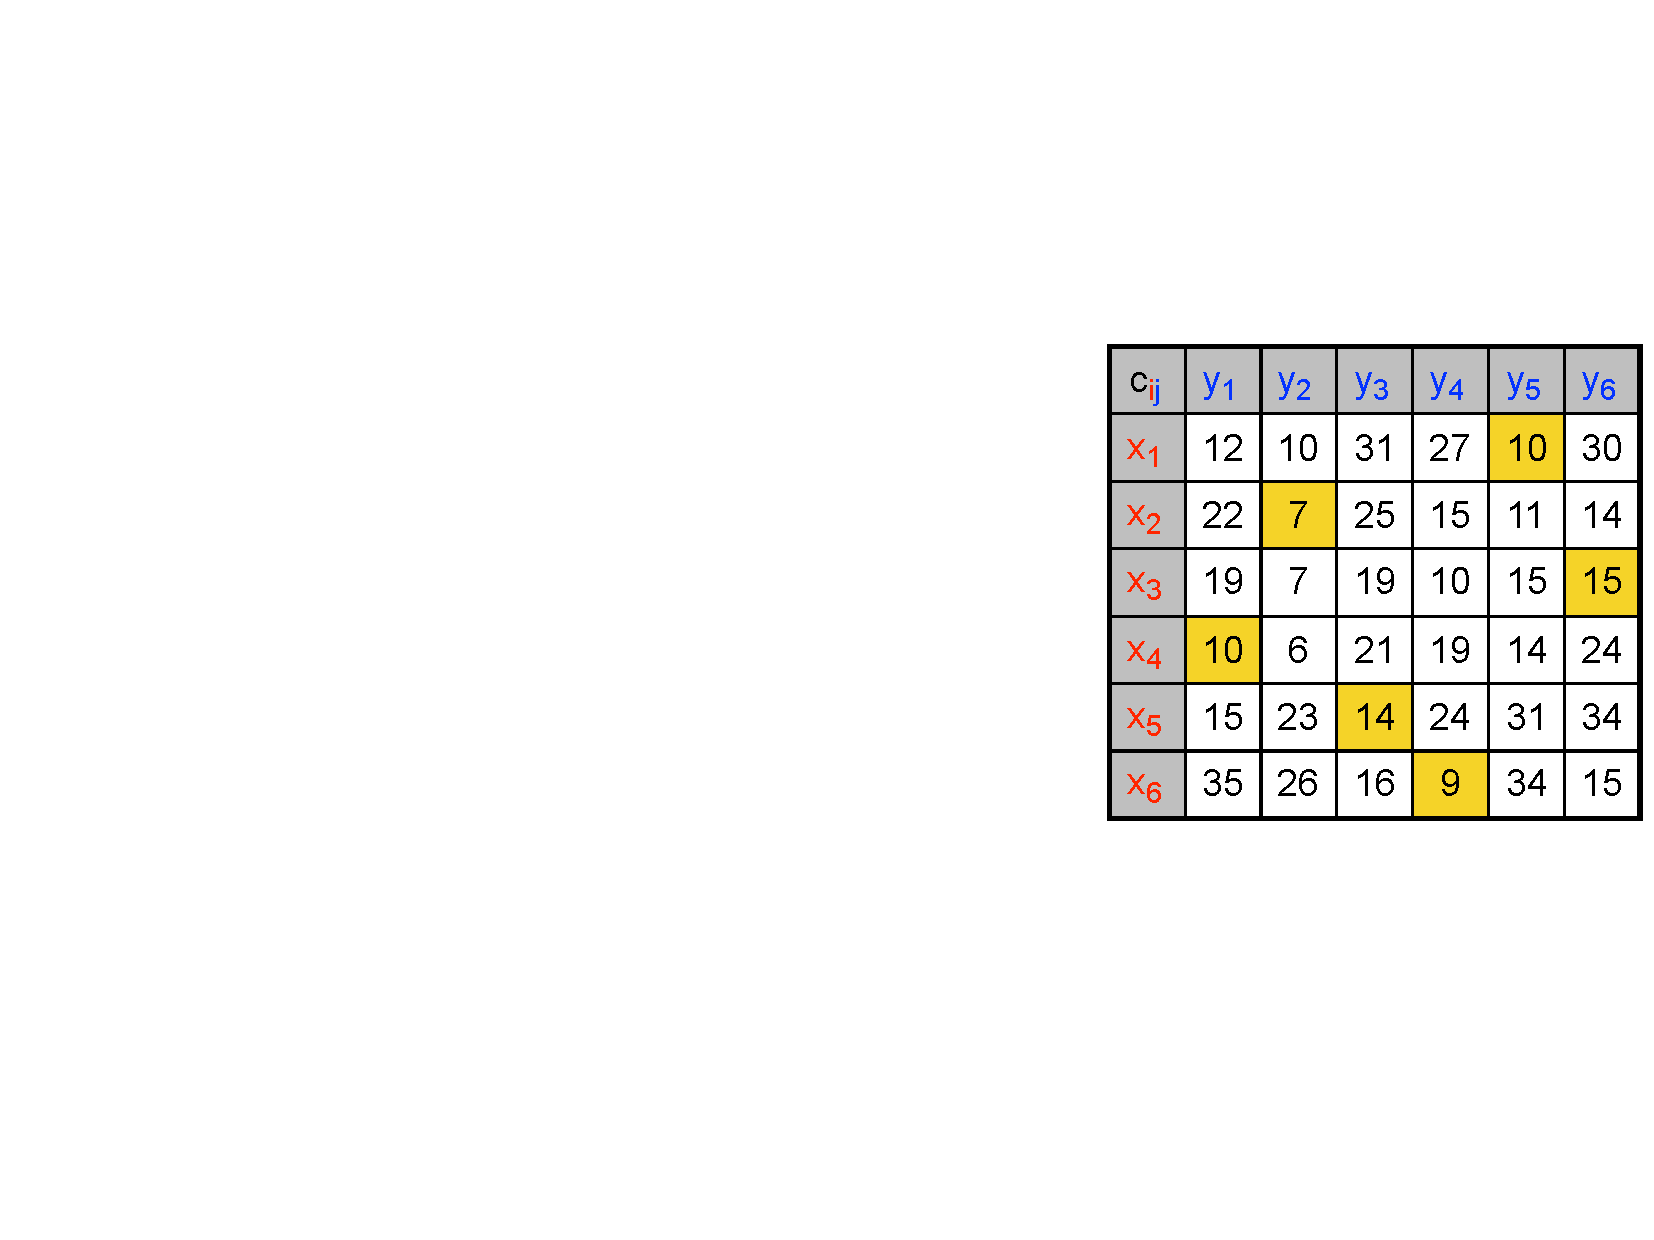
\includegraphics[width=.22\linewidth]{transport/cafe-paris/map-paris-1-couts} 
        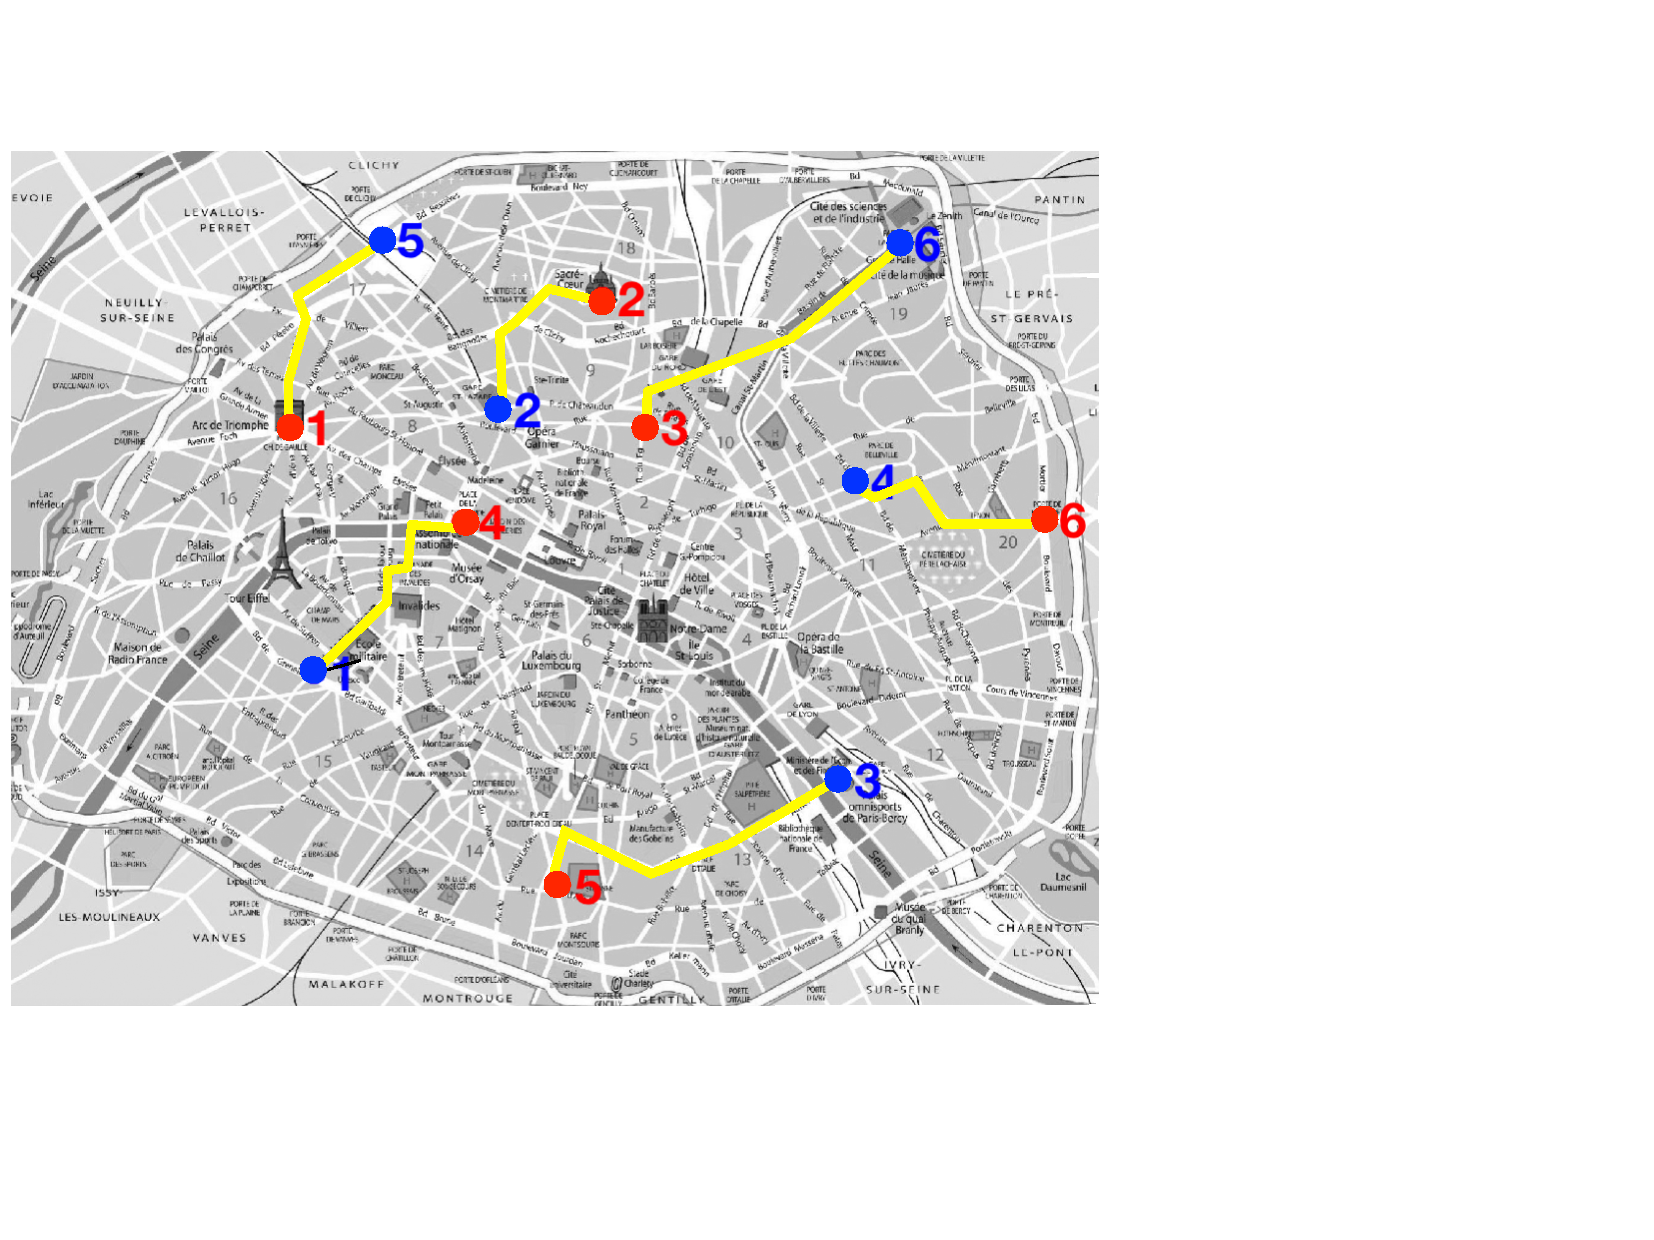
\includegraphics[width=.27\linewidth]{transport/cafe-paris/map-paris-1} 
    \end{tabular}
    \caption{\label{fig:image-cafe} Matrice de coût et connexions associées. Gauche : une ligne de la matrice coût. Droite : un exemple particulier de permutation. } 
\end{figure}

Afin de satisfaire la contrainte d'approvisionnement (que l'on appelle aussi la conservation de la masse), il faut que chaque boulangerie soit connectée à un et un seul café. Comme il y a le même nombre de boulangeries que de cafés, ceci implique que chaque café est également connecté à une et une seule boulangerie. On va noter 
\eq{    
    \si : \iC \in \{1,\ldots,6\} \longmapsto \jC \in \{1,\ldots,6\}
}
un tel choix de connexions. 
%
Les deux images de droite de la figure~\ref{fig:image-cafe} illustrent l'exemple
\eql{\label{eq-bijection-exmp}
    \si(\Red{1})=\Blu{5}, \;
    \si(\Red{2})=\Blu{2}, \;
    \si(\Red{3})=\Blu{6}, \;
    \si(\Red{4})=\Blu{1}, \;
    \si(\Red{5})=\Blu{3}, \;
    \si(\Red{6})=\Blu{4}.
}  
La contrainte de conservation de masse signifie que $\si$ est une bijection de l'ensemble $\{1,\ldots,6\}$ dans lui-même. On dit aussi que $\si$ est une permutation. 

Le coût de transport associé à une telle bijection est la somme des coûts $C_{\iC,\si(\iC)}$ sélectionnés par la permutation $\si$, c'est-à-dire 
\eql{\label{eq:cout}
    \text{Coût}(\si) \eqdef 
        C_{\Red{1},\si(\Red{1})} + 
        C_{\Red{2},\si(\Red{2})} + 
        C_{\Red{3},\si(\Red{3})} + 
        C_{\Red{4},\si(\Red{4})} + 
        C_{\Red{5},\si(\Red{5})} + 
        C_{\Red{6},\si(\Red{6})}. 
}
Par exemple, pour la bijection~\eqref{eq-bijection-exmp} montrée à la figure~\ref{fig:image-cafe}, on obtient comme coût
\eq{
    C_{\Red{1},\Blu{5}} + 
    C_{\Red{2},\Blu{2}} + 
    C_{\Red{3},\Blu{6}} + 
    C_{\Red{4},\Blu{1}} + 
    C_{\Red{5},\Blu{3}} + 
    C_{\Red{6},\Blu{4}} = 
    10 + 7 + 15 + 10 + 14 + 9 = 65. 
}


Le problème de Monge consiste à chercher une permutation $\si$ qui a le coût minimum, c'est-à-dire résoudre le problème d'optimisation
\eql{\label{eq:monge}
    \umin{\si \in \Si_6} \text{Coût}(\si), 
}
où 
l'on a noté $\Si_6$ 
l'ensemble des permutations de l'ensemble $\{1,\ldots,6\}$.

\begin{figure}\centering
    \begin{tabular}{@{}c@{\hspace{1mm}}c@{\hspace{1mm}}c@{\hspace{1mm}}c@{}}
        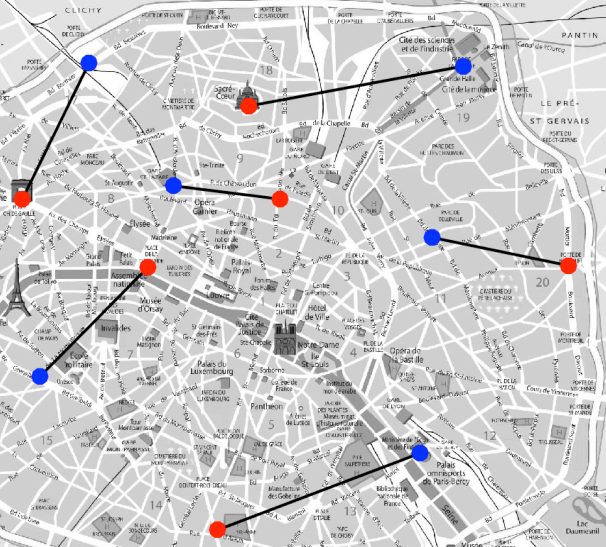
\includegraphics[width=.22\linewidth]{transport/cafe-paris/ordre-croissant-64}&
        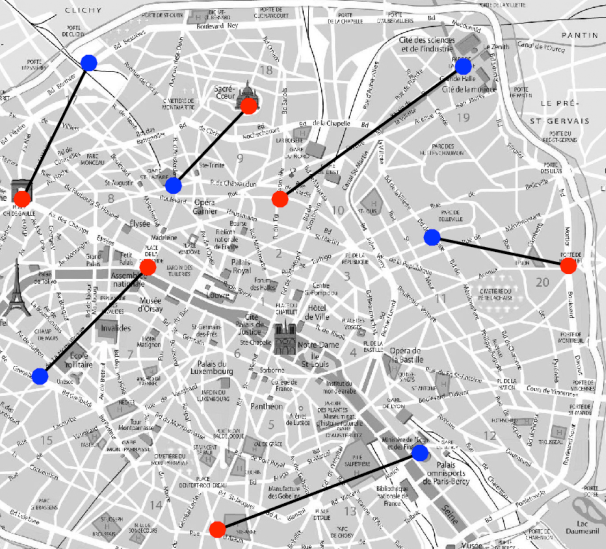
\includegraphics[width=.22\linewidth]{transport/cafe-paris/ordre-croissant-65}&
        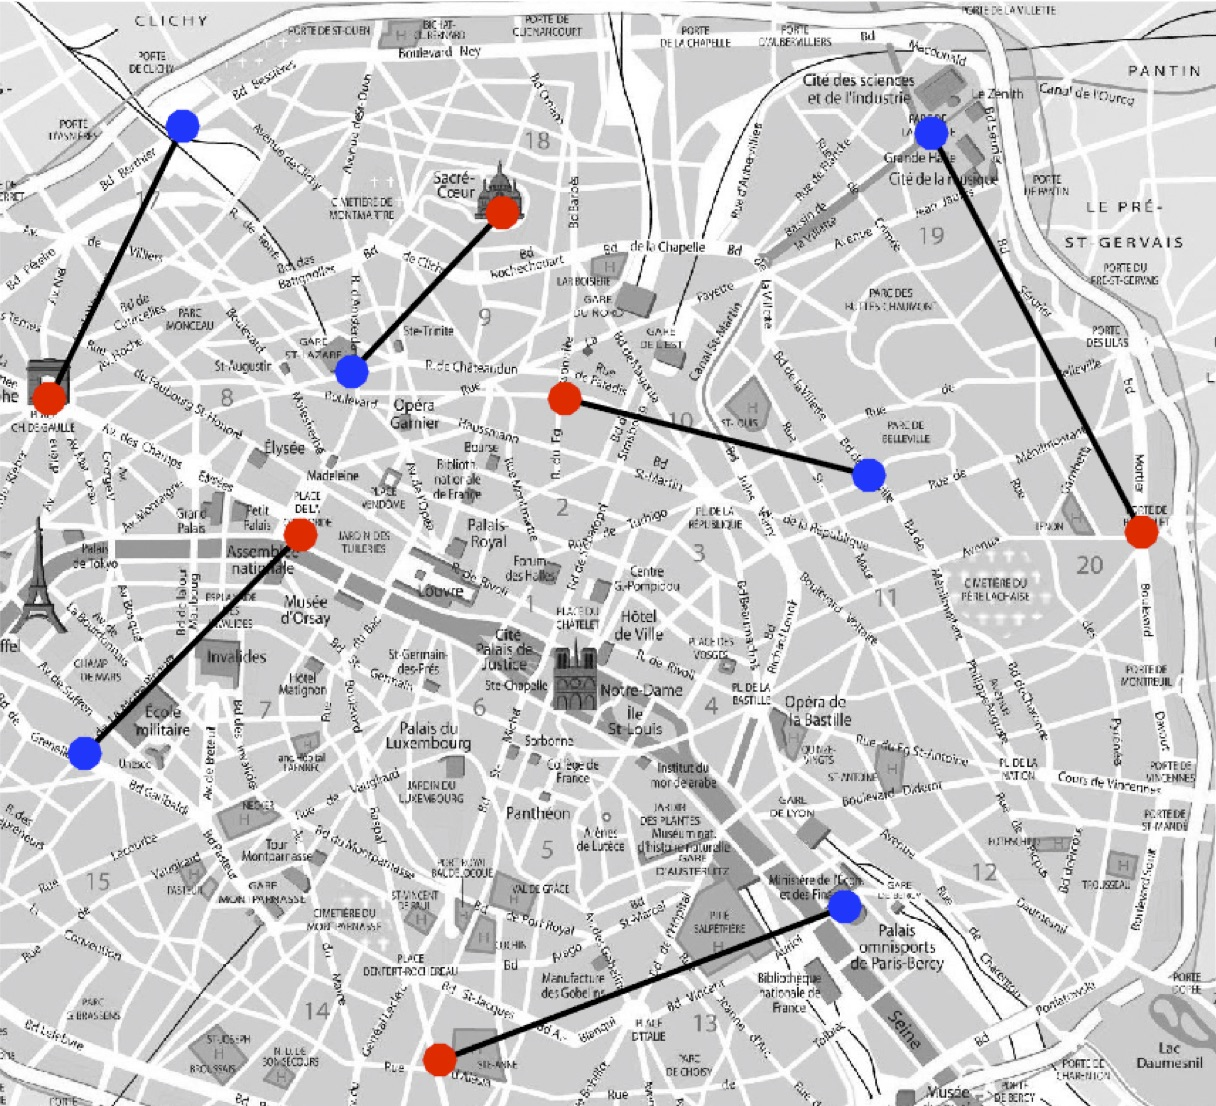
\includegraphics[width=.22\linewidth]{transport/cafe-paris/ordre-croissant-66}&
        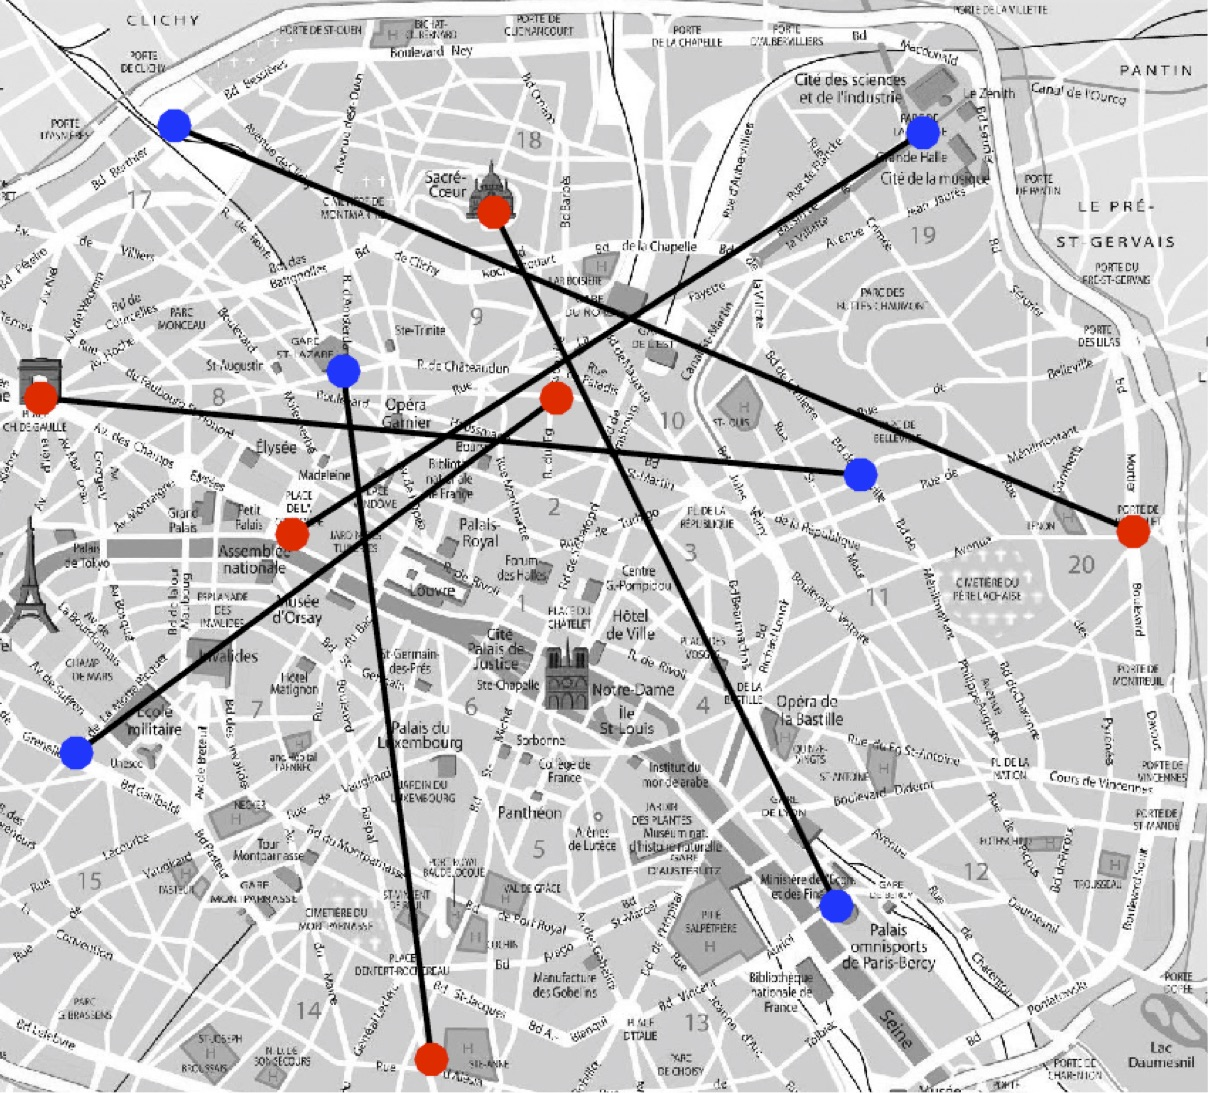
\includegraphics[width=.22\linewidth]{transport/cafe-paris/ordre-croissant-152}\\
        Coût=64 &  
        Coût=65 &  
        Coût=66 &  
        Coût=152
    \end{tabular}
    \caption{\label{fig:ordre-croissant} Exemples de permutations avec différent coûts. } 
\end{figure}

La figure~\ref{fig:ordre-croissant} montre que la permutation~\eqref{eq-bijection-exmp} n'est pas la meilleure : il existe par exemple une autre permutation qui a un coût de 64. Mais est-ce la meilleure ? Il se trouve que oui, on peut en effet tester sur un ordinateur toutes les permutations de  $\{1,\ldots,6\}$ et calculer leur coût. Combien y a-t-il de permutations au total ? Pour effectuer ce dénombrement, on voit qu'il y a six choix d'affectation possible de $\Red{1}$ à  $\si(\Red{1}) \in \{\Blu{1,\ldots,6}\} $, puis cinq choix possibles pour affecter $\Red{2}$ à $\si(\Red{2}) \in  \{ \Blu{1,\ldots,6 } \}  - \{ \si(\Red{1}) \}$, et ainsi de suite. Le nombre total de possibilités est donc $6 \times 5 \times 4 \times 3 \times 2 \times 1 = 720$ que l'on note $6!$. Si l'on considère un nombre $n$ de boulangeries, alors le nombre de permutations à tester pour trouver la meilleure est $n! =n \times (n-1) \times \cdots \times 2 \times 1$. Ce nombre croît extrêmement vite avec $n$, par exemple $70! \approx 1,198 \times 10^{100}$, à comparer avec les $10^{11}$ neurones dans le cerveau et les $10^{79}$ atomes dans l'univers. Cette stratégie de recherche exhaustive n'est donc possible que pour de toute petites valeurs de $n$. 


\begin{figure}\centering
    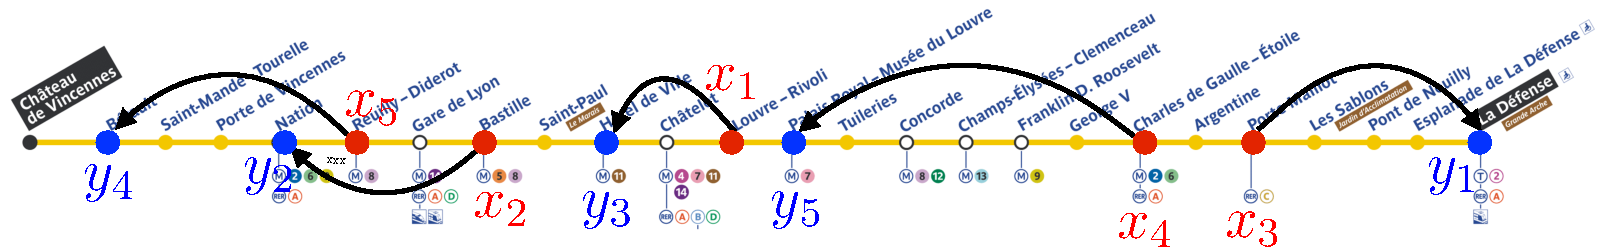
\includegraphics[width=.9\linewidth]{transport/metro/plan-metro}
    \caption{\label{fig:metro} Le transport optimal en 1D le long d'une ligne de métro. La bijection optimale est  
    $\si : (\Red{1,2,3,4,5}) \mapsto (\Blu{3,4,5,1,2})$. } 
\end{figure}

%%%%%%%%%%%%%%%%%%%%%%%%%%%%%%%
\myparagraph{En 1D et 2D}

% ENLEVE : % La section~\ref{sec-kanto} explique comment des avancées mathématiques ont permis de développer des techniques efficaces pour calculer un transport optimal $\si$ même pour de grandes valeurs de $n$. Mais il aura fallu attendre près de 200 ans pour y arriver. Dans quelques rares cas, on peut cependant calculer le transport optimal de façon simple. 

Il aura fallu près de 200 ans pour que des idées nouvelles émergent pour calculer efficacement un transport optimal $\sigma$ même pour des grandes valeurs de $n$. Avant d'expliquer ces avancées mathématiques, commençons par un cas dans lequel le transport optimal se calcule facilement.
%
Le cas le plus élémentaire est lorsque les points à apparier sont le long d'un axe 1D, par exemple si les cafés et les boulangeries sont situés le long d'une ligne de métro. Il faut également que le coût $C_{\iC,\jC}$ soit la distance le long de cet axe (par exemple le temps de trajet en métro entre les stations). 
%
On se place à gauche de tous les points en jeu et on parcourt la ligne de métro de gauche à droite. Le premier point rouge est associé avec le premier point bleu, le deuxième point rouge avec le deuxième point bleu, etc. 
%
% Dans ce cas, il suffit de reclasser les indices $\iC$ et $\jC$ par ordre croissant (donc de gauche à droite le long de la ligne de métro) et d'apparier le premier indice $\iC$ au premier indice $\jC$ ensemble, puis le deuxième indice, etc. 
%
Ce procédé est illustré à la figure~\ref{fig:metro}.  
%
Le temps de calcul nécessaire pour calculer le transport optimal en métro est donc le temps nécessaire pour classer les indices. L'algorithme le plus simple pour effectuer un classement est celui utilisé habituellement pour trier un jeu de $n$ cartes : il s'agit du tri par insertion, qui insère itérativement chaque carte à sa place par rapport aux cartes déjà classées. Il effectue $n(n-1)/2$ comparaisons. Pour $n=70$, ceci nécessite donc seulement 2415 operations, ce qui rend la méthode utilisable, au contraire de la recherche exhaustive de toutes les $n!$ permutations.
% 
On dispose d'algorithmes encore plus rapides (par exemple le tri fusion), qui effectuent de l'ordre de $n \log(n)$ opérations, et donc pour $n = 70$, de telles méthodes nécessitent moins de 1000 opérations. 

Malheureusement, il n'est plus possible d'utiliser cette technique de classement dans des cas plus généraux. Pour des points en dimension 2, si on prend comme coût $C_{\iC,\si(\iC)}$ la distance euclidienne (la distance en vol d'oiseau) entre les points, alors Gaspard Monge a montré dans son papier original (voir la figure~\ref{fig:ot2d}, à gauche) qu'un transport optimal ne peut pas contenir de croisement. Par exemple, comme le montre la figure~\ref{fig:ot2d} (à droite), si l'on trace tous les segments entre les points $\iC \mapsto \jC = \si(\iC)$  que l'on relie par la bijection définie par un $\si$ optimal, ceux-ci ne se croisent jamais. 

\begin{figure}\centering
    \begin{tabular}{@{}c@{\hspace{6mm}}c@{\hspace{3mm}}c@{}} % c@{\hspace{1mm}}
        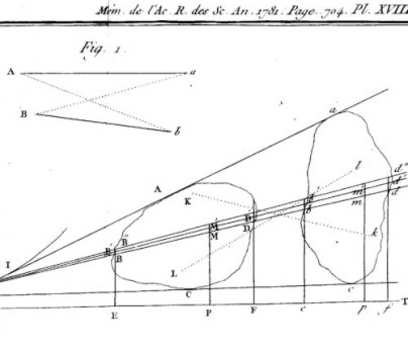
\includegraphics[width=.22\linewidth]{transport/monge-2d/article-monge}&
%        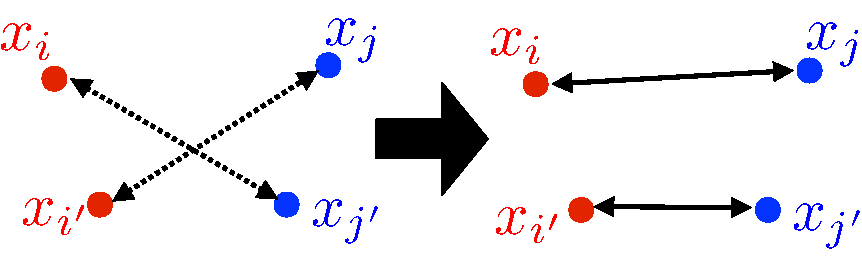
\includegraphics[width=.22\linewidth]{transport/monge-2d/decroisement}&
        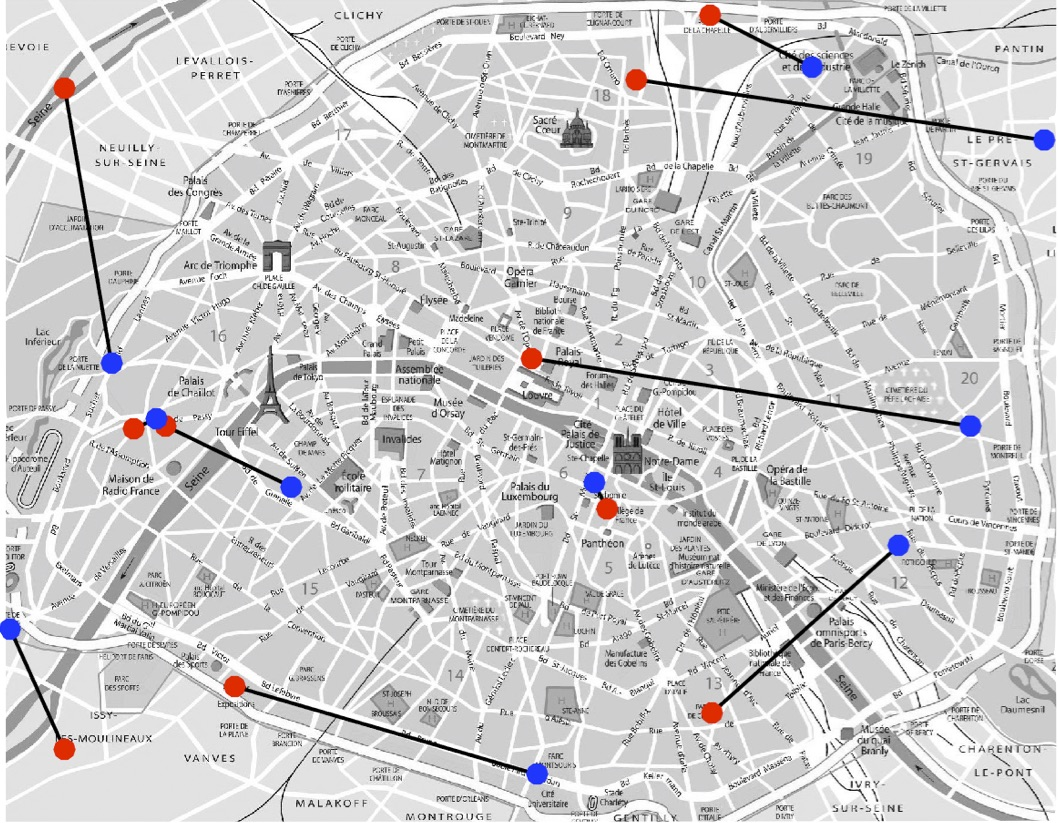
\includegraphics[width=.22\linewidth]{transport/monge-2d/example-10}&
        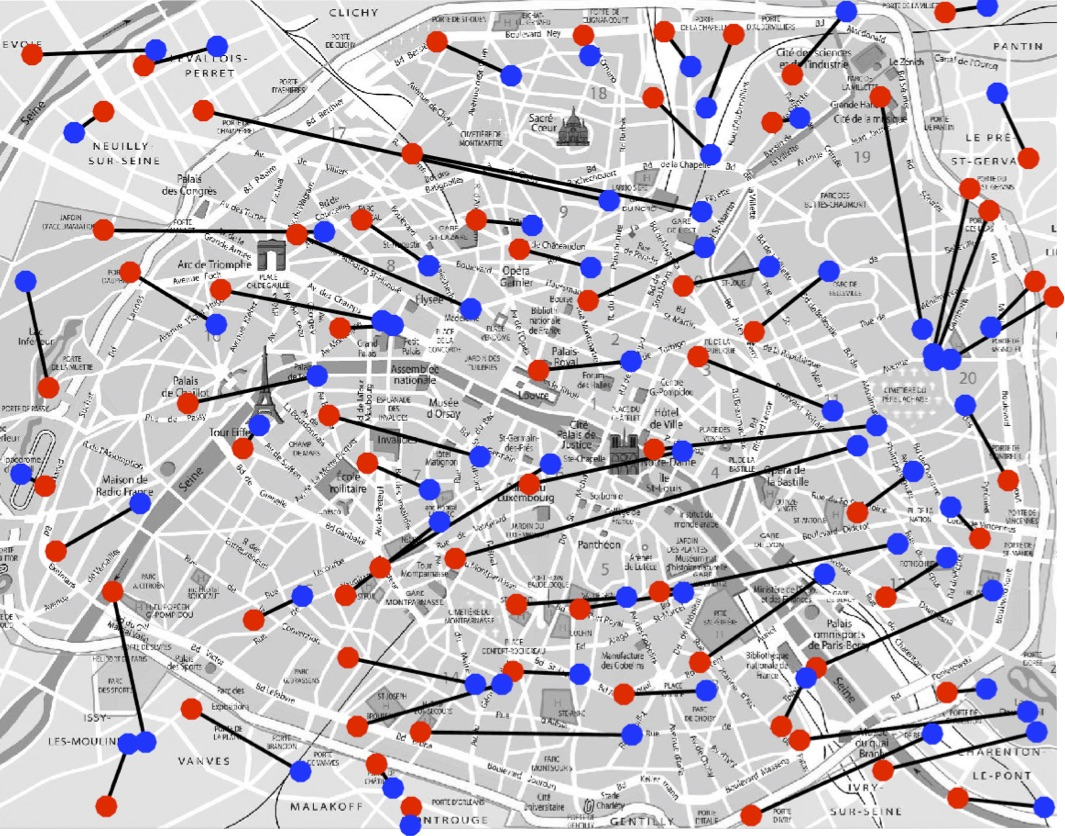
\includegraphics[width=.22\linewidth]{transport/monge-2d/example-70}
    \end{tabular}
    \caption{\label{fig:ot2d} Gauche: extrait de l'article de Monge~\cite{Monge1781}. Droite: le transport optimal en 2D pour un coût euclidien.  } 
\end{figure}

Cette observation géométrique n'est cependant pas suffisante pour calculer un transport optimal en 2D : il existe en effet beaucoup de permutations $\si$ telles que les segments associés ne se croisent pas. 
%
Il va falloir analyser de façon plus fine la structure des permutations optimales afin de pouvoir les calculer de façon efficace. 
%
Nous allons maintenant voir comment Leonid Kantorovitch a reformulé le problème de Monge afin d'y parvenir. 


%%%%%%%%%%%%%%%%%%%%%%%%%%%%%%%%%%%%%%%%%%%%%%
\section{Le Transport Optimal de Kantorovitch}
\label{sec-kanto}

Leonid Kantorovitch est un mathématicien et économiste soviétique qui a révolutionné la théorie du transport optimal pendant les années 40. Ses recherches sont issues de considérations pratiques qui l'ont occupé avant et après la seconde guerre mondiale. Il y a joué un rôle important pour assurer une distribution optimale des ressources, en particulier durant le siège de Léningrad.
%
Il a par la même occasion participé au développement de l'optimisation moderne, laquelle a eu un impact énorme dans de très nombreux domaines appliqués. Il a ainsi obtenu en 1975 le prix Nobel d'économie, car les premières applications (mais certainement pas les seules !) de sa théorie se sont manifestées dans ce domaine. 


%%%%%%%%%%%%%%%%%%%%%%%%%%%%%%%
\myparagraph{Le problème de Kantorovitch}

L'idée centrale de Kantorovitch~\cite{Kantorovich42} est de modifier le problème de Monge en remplaçant l'ensemble des permutations par un ensemble plus grand mais plus simple. Tout d'abord on remarque que l'on peut représenter une permutation $\si \in \Si_n$ à l'aide d'une matrice de permutation $P$ qui est une matrice binaire (remplie de 0 et de 1) de taille $n \times n$ telle que $P_{\iC,\jC} = 0$ sauf si $\jC=\si(\iC)$ auquel cas $P_{\iC,\si(\iC)} = 1$. Par exemple, pour $n=3$ points, les permutations 
$(\Red{1,2,3}) \mapsto (\Blu{1,2,3})$ (l'identité), 
$(\Red{1,2,3}) \mapsto (\Blu{3,2,1})$ et
$(\Red{1,2,3}) \mapsto (\Blu{2,1,3})$ sont respectivement représentées par les matrices de taille $3 \times 3$
\eq{
	\begin{pmatrix} 1&0&0 \\ 0&1&0 \\ 0&0&1 \end{pmatrix}, \quad
	\begin{pmatrix} 0&0&1 \\ 0&1&0 \\ 1&0&0 \end{pmatrix} \qetq
	\begin{pmatrix} 0&1&0 \\ 1&0&0 \\ 0&0&1 \end{pmatrix}.
}
Dans la suite, on note $\Pp_n$ l'ensemble des $n!$ matrices de permutation de taille $n \times n$.

Comme la matrice est binaire, avec seulement $n$ éléments non nuls égaux à 1, on peut remplacer la somme de $n$ termes qui apparait dans $\text{Coût}(\si)$ défini en~\eqref{eq:cout} par une somme sur l'ensemble des $n \times n$ indices $(\iC,\jC)$, c'est-à-dire que si $P$ est la matrice de permutation associée à $\si$, on a 
\eq{
	\text{Coût}(\si) = \sum_{\iC=1}^n \sum_{\jC=1}^n P_{\iC,\jC} C_{\iC,\jC}.
}
On peut ainsi remplacer le problème de Monge~\eqref{eq:monge} par le problème équivalent 
\eql{\label{eq:mongematrix}
    \umin{P \in \Pp_n}  \sum_{\iC=1}^n \sum_{\jC=1}^n P_{\iC,\jC} C_{\iC,\jC}.
}

Le génie de Kantorovitch a été de remarquer que l'on peut remplacer l'ensemble discret $\Pp_n$ (c'est-à-dire composé d'un ensemble fini, mais très grand, de $n!$ matrices) par un ensemble \guill{continu} (donc en particulier infini) mais plus simple. On remarque en effet que les matrices de permutation de $\Pp_n$ sont exactement les matrices qui ont un et un seul 1 le long de chaque ligne et de chaque colonne. Ceci peut aussi s'exprimer comme le fait qu'une matrice de permutation est une matrice binaire dont la somme de chaque ligne et de chaque colonne vaut 1, c'est-à-dire
\eq{
	\Pp_n = \enscond{ P \in \{0,1\}^{n \times n} }{ \foralls \iC, \sum_{\jC} P_{\iC,\jC}=1, \foralls \jC, \sum_{\iC} P_{\iC,\jC}=1  }.
}
Ce qui rend cet ensemble très compliqué, c'est la contrainte binaire, c'est-à-dire que ces matrices sont contraintes à être dans $\{0,1\}^{n \times n}$. Kantorovitch propose alors de \guill{relaxer} cette contrainte en supposant simplement que les entrées de $P$ sont entre $0$ et $1$. Ceci définit un ensemble plus grand, l'ensemble des matrices bistochastiques 
\eql{\label{eq:bistoch}
	\Bb_n \eqdef \enscond{ P \in [0,1]^{n \times n} }{ \foralls \iC, \sum_{\jC} P_{\iC,\jC}=1, \foralls \jC, \sum_{\iC} P_{\iC,\jC}=1  }.
}
Le problème de Kantorovitch s'obtient en effectuant ce remplacement dans~\eqref{eq:mongematrix}, afin de résoudre 
\eql{\label{eq:kantoassign}
    \umin{P \in \Bb_n} 
        \sum_{\iC=1}^n \sum_{\jC=1}^n P_{\iC,\jC} C_{\iC,\jC}.
}
L'immense avantage du problème de Kantorovitch~\eqref{eq:kantoassign} par rapport à celui de Monge~\eqref{eq:mongematrix} est que l'ensemble des matrices bistochastique est convexe, c'est-à-dire que si l'on considère deux matrices bistochastiques $P,Q \in \Bb_n$, alors leur moyenne $\frac{P+Q}{2} \in \Bb_n$ est encore bistochastique. Ceci n'est pas vrai pour les matrices de permutation, puisque la moyenne de deux matrices binaires $(P,Q)$ n'est pas binaire (sauf bien sûr si $P=Q$). Cette convexité est la clef pour le développement d'algorithmes efficaces. 
%
Cette nouvelle formulation a en effet pu bénéficier d'une deuxième révolution initiée par George Dantzig~\cite{Dantzig51}, qui, à la même époque, a proposé l'algorithme du simplexe. Celui-ci permet de résoudre efficacement une certaine classe de problèmes d'optimisation convexe : les problèmes de programmation linéaire, dont~\eqref{eq:kantoassign} est un cas particulier. Dans le cas du problème de Kantorovitch, il existe en effet un algorithme du simplexe qui a une complexité de l'ordre de $n^3$ opérations, ce qui permet de faire des calculs pour de grands $n$, de l'ordre de plusieurs milliers. 


%%%%%%%%%%%%%%%%%%%%%%%%%%%%%%%
\myparagraph{L'équivalence Monge--Kantorovitch}

L'ensemble des matrices bistochastiques est plus grand que celui des matrices de permutations, $\Pp_n \subset \Bb_n$, de sorte que l'on a l'inégalité 
\eql{\label{eq:monge-vs-kanto}
    \umin{P \in \Bb_n} 
        \sum_{\iC=1}^n \sum_{\jC=1}^n P_{\iC,\jC} C_{\iC,\jC}
     \leq 
    \umin{P \in \Pp_n} 
        \sum_{\iC=1}^n \sum_{\jC=1}^n P_{\iC,\jC} C_{\iC,\jC}
}
entre les problèmes de Kantorovitch et de Monge. Mais de façon à première vue surprenante, un théorème fondamental dû à George Birkhoff et à John von Neumann~\cite{birkhoff,von1953certain} assure qu'en fait il y a égalité entre les valeurs de ces deux minimisations. En effet, ce théorème montre qu'il existe toujours une matrice solution du problème de Kantorovitch qui est une matrice de permutation, de sorte qu'elle est aussi solution du problème de Monge. Attention cependant, en général il n'y a pas unicité des solutions de ces problèmes : il peut exister une matrice bistochastique solution du problème de Kantorovitch qui n'est pas une permutation. 
%
La conjonction de deux avancées spectaculaires, dues à Kantorovitch et à Dantzig, a permis de rendre le transport optimal applicable à des problèmes de grande taille, puisque l'algorithme du simplexe permet de résoudre en pratique ces problèmes. 

%%%%%%%%%%%%%%%%%%%%%%%%%%%%%%%
\myparagraph{Le cas pondéré}

Outre son intérêt pratique, la formulation de Kantorovitch a aussi permis de généraliser le problème initial de Monge, en donnant le bon cadre pour le formaliser et l'étudier mathématiquement. En effet, le problème de Monge est très limité. Que se passe-t-il par exemple s'il n'y pas le même nombre $n$ de cafés et $m$ de boulangeries ? Le problème initial~\eqref{eq:monge} n'a pas de solution, car on ne peut pas mettre en bijection deux ensembles de tailles différentes. Le bon concept n'est pas le nombre de boulangeries et de cafés, mais plutôt les distributions $(\Red{a_1,\ldots,a_n})$ de production (associées au boulangeries) et les distributions $(\Blu{b_1,\ldots,b_m})$ de consommation des cafés. 
%
Par exemple, si la première boulangerie produit 45 croissants par jour, on prendra $\Red{a_1} =45$, de même $\Blu{b_3} = 34$ signifie que le 3$^\text{e}$ café consomme 34 croissants par jour.
%
Dans le cas initialement considéré, où $n=m$, toutes les quantités $\Red{a_i}$ et $\Blu{b_j}$ sont égales à 1. Mais dans de nombreux cas concrets, ces quantités sont quelconques. Ces quantités doivent être positives, et vérifier 
\eq{
	\Red{a_1+\cdots+a_n} = \Blu{b_1 + \cdots + b_m}, 
}
de sorte qu'il y ait autant de production que de consommation. La construction de Kantorovitch s'adapte naturellement à ce cas de distributions générales, en remplaçant les matrices bistochastiques~\eqref{eq:bistoch} par des matrices de \guill{couplage} qui satisfont la contrainte de conservation de la masse 
\eq{
	\Bb(\aC,\bC) \eqdef \enscond{ P \in \RR_+^{n \times m} }{ \foralls \iC, \sum_{\jC} P_{\iC,\jC}=\Red{a_i}, \foralls \jC, \sum_{\iC} P_{\iC,\jC}= \Blu{b_j}  }.
}
Dans le cas initial où $n=m$ et $\Red{a_i}=\Blu{b_j}=1$, alors $\Bb(\aC,\bC) = \Bb_n$ et l'on retrouve des matrices bistochastiques. Dans le cas général, à chaque fois qu'une entrée $P_{\iC,\jC}$ est non-nulle, ceci signifie que l'on transfère de la \guill{masse} (ici une certaine quantité de croissants) entre $\iC$ et $\jC$. Comme le montre la figure~\ref{fig:coupling-visu}, on peut visualiser de différentes façons une telle matrice $P$ couplant deux distributions $(\aC,\bC)$.
%
Contrairement au cas des matrices bistochastiques, pour lequel il y a toujours une solution qui est une permutation, ici un couplage optimal $\Bb(\aC,\bC)$ peut avoir plus d'une seule entrée non-nulle $P_{\iC,\jC}$ le long d'une ligne indexée par $\iC$ (voir la figure~\ref{fig:coupling-visu}). Ceci signifie que cette boulangerie $\iC$ est connectée à plusieurs cafés, de sorte que sa production est alors séparée en plusieurs lots de croissants distribués, tout en satisfaisant la contrainte de conservation de la masse $\sum_{\jC} P_{\iC,\jC}=\Red{a_i}$.

\begin{figure}\centering
    \begin{tabular}{@{}c@{\hspace{1mm}}c@{\hspace{1mm}}c@{\hspace{1mm}}c@{}}
        \includegraphics[width=.22\linewidth]{transport/kantorovitch/coupling-array}&
        \includegraphics[width=.22\linewidth]{transport/kantorovitch/coupling-squares}&
        \includegraphics[width=.22\linewidth]{transport/kantorovitch/coupling-map}&
        \includegraphics[width=.22\linewidth]{transport/kantorovitch/coupling-bipartite} \\
        (a) matrice & (b) histogrammes & (c) segments & (d) graphe biparti
    \end{tabular}
    \caption{\label{fig:coupling-visu} Différentes façons de représenter une matrice de couplage $P \in \Bb(\aC,\bC)$:
    	(a) un tableau de nombres dont les lignes et colonnes ont des sommes prescrites ; 
		(b) un histogramme bidimensionnel dont la taille de carré est proportionnelle à $P_{\iC,\jC}$ ; 
		(c) un ensemble de segments dont la largeur est proportionnelle à $P_{\iC,\jC}$. 
		(d) un graphe biparti, c'est-à-dire avec deux groupes de points reliés par des arêtes.   } 
\end{figure}


Le problème de Kantorovitch qui généralise~\eqref{eq:kantoassign} s'écrit alors
\eql{\label{eq-kanto-gen}
    \umin{P \in \Bb(\aC,\bC)} 
        \sum_{\iC=1}^n \sum_{\jC=1}^m P_{\iC,\jC} C_{\iC,\jC}
}
ce qui signifie que l'on doit payer un coût  $C_{\iC,\jC}$ à chaque fois que l'on transfère une unité de masse entre $\iC$ et $\jC$. Tout comme le problème original~\eqref{eq:kantoassign}, on peut le résoudre de façon efficace avec l'algorithme du simplexe.  La figure~\ref{fig:coupling-visu} montre un exemple de couplage optimal. 



%%%%%%%%%%%%%%%%%%%%%%%%%%%%%%%%%%%%%%%%%%%%%%
\section{Les applications}

Bien que les motivations initiales de Monge et Kantorovitch aient été respectivement militaires et économiques, le transport optimal a trouvé d'innombrables applications, à la fois théoriques et concrètes. Sur le plan mathématique, on peut considérer des distributions \guill{continues} de masses, en quelque sorte la limite quand le nombre de points $n$ tend vers l'infini. Ceci permet de définir le problème de transport entre des mesures de probabilités quelconques. Ce point de vue théorique est extrêmement fructueux, et c'est le mathématicien français Yann Brenier qui a le premier montré l'équivalence dans le cadre continu des formulations de Monge et de Kantorovich~\cite{Brenier91}. Ces travaux pionniers ont montré la connexion entre le problème de transport et les équations aux dérivées partielles, et ont débouché, entre autres, sur les médailles Fields de Cédric Villani (2010) et Alessio Figalli (2018). 

\begin{figure}\centering
\begin{tabular}{@{}c@{\hspace{1mm}}c@{\hspace{1mm}}c@{}}
    \includegraphics[width=.24\linewidth]{transport/applis/painting-2} &
    \includegraphics[width=.24\linewidth]{transport/applis/painting-1} &
    \includegraphics[width=.24\linewidth]{transport/applis/painting-2-equalized} \\
    Image $(\Red{x_i})_{\iC=1}^n$ & Image $(\Blu{y_j})_{\jC=1}^n$ & Image  $(y_{\si(\iC)})_{\iC=1}^n$ \\
    \includegraphics[width=.24\linewidth]{transport/applis/painting-2-histo}&
    \includegraphics[width=.24\linewidth]{transport/applis/painting-1-histo}&
    \includegraphics[width=.24\linewidth]{transport/applis/painting-1-histo}
\end{tabular}
\caption{\label{fig:image-eq} Exemple de transfert de palettes de couleurs à l'aide du transport optimal. 
	Haut: les pixels sont sur la grille d'affichage pour former une image couleur. 	
	Bas: les pixels sont placés à leurs positions dans $\RR^3$ pour former un nuage de points. }
\end{figure}

Le transport optimal est depuis peu au c\oe{}ur de problématiques plus appliquées en sciences des données, en particulier pour résoudre des problèmes en traitement d'image et en apprentissage machine. 
%
La première idée, la plus immédiate, est d'utiliser la bijection $\si$ afin de transformer des données, par exemple des images. Dans ce cas, on considère les pixels $(\Red{x_i})_{\iC=1}^n$ et $(\Blu{y_j})_{\jC=1}^n$ de deux images couleur. Chaque pixel $\Red{x_i}, \Blu{y_j} \in \RR^3$ est un vecteur de dimension 3, qui représente les intensités de chacune des trois couleurs élémentaires, rouge, vert et bleu. Afin de changer les couleurs de la première image, et lui imposer la palette de la deuxième image, on calcule le transport $\si$ pour la matrice de coût $C_{\iC,\jC} = \norm{\Red{x_i} - \Blu{y_j}}^2$ (c'est-à-dire le carré de la norme euclidienne dans $\RR^3$), c'est-à-dire le carré de la distance euclidienne entre les pixels. L'image avec les couleurs modifiées est $(y_{\si(\iC)})_{\iC=1}^n$, c'est à dire que l'on remplace dans la première image le pixel $\Red{x_i}$ par le pixel $y_{\si(\iC)}$. Cette image ressemble à la première, mais a la palette de couleurs de la deuxième image.
%
La figure~\ref{fig:image-eq} illustre ce procédé pour imposer la palette de couleurs de Picasso à un tableau de Cézanne. 

On peut également utiliser le transport optimal pour des problèmes plus difficiles, en n'utilisant que de façon indirecte la bijection $\si$ ou bien la matrice de couplage optimal $P \in \Bb(\aC,\bC)$. L'idée centrale est que la quantité associée à un couplage optimal $P$ solution de~\eqref{eq-kanto-gen}
\eq{
	W(\aC,\bC) \eqdef \sum_{i,j} P_{\iC,\jC} C_{\iC,\jC}
}
définit en quelque sorte l'effort nécessaire pour déplacer la masse de la distribution $\aC$ vers la distribution $\bC$. Elle permet donc de quantifier combien ces deux distributions sont \guill{proches}. Par exemple, si $C_{\iC,\jC} = \norm{\Red{x_i} - \Blu{y_j}}^2$ est le carré de la distance euclidienne entre des points, alors la quantité $W(\aC,\bC)^{1/2}$ est une distance entre les distributions, en particulier elle vérifie $W(\aC,\bC)=0$ si et seulement si $\aC=\bC$, et elle vérifie l'inégalité triangulaire. Ces propriétés sont très importantes pour permettre d'appliquer le transport à des problèmes pratiques.


\begin{figure}\centering
        \includegraphics[width=.6\linewidth]{transport/applis/shapes-3d}
    \caption{\label{fig:barycenters} Exemple d'interpolation barycentrique entre des formes 3D, obtenu en minimisant~\eqref{eq-bary}.  }
\end{figure}

Un exemple typique d'application de cette quantité $W$ consiste à calculer des barycentres entre des distributions~\cite{agueh2011barycenters}. La figure~\ref{fig:barycenters} montre un exemple où l'on considère trois distributions $a,b,c$ (montrées aux trois sommets du triangles) qui sont des distributions uniformes de masse à l'intérieur de formes 3D (c'est-à-dire que la masse $a_i$ associée au $i^{\text{e}}$ point est 0 à l'extérieur de la première forme et prend une valeur constante à l'intérieur). 
%
On calcule un barycentre pondéré de ces trois distributions en imitant le fait que dans un espace Euclidien, le barycentre pondéré $r$ de trois points $x,y,z$ minimise la somme des distances au carré
\eq{
    \umin{r} \al \norm{x-r}^2 + \be \norm{y-r}^2 +  \ga \norm{z-r}^2,
}
où les poids $(\al,\be,\ga)$ sont les pondérations du barycentre, qui sont des réels positifs et tels que $\al+\be+\ga=1$.
%
Le barycentre pondéré $d$  de $(a,b,c)$ minimise ainsi la somme pondérée de distances de transport optimal
\eql{\label{eq-bary}
	\umin{d} \al W(a,d) + \be W(b,d) + \ga W(c,d).
}
En modifiant les poids $(\al,\be,\ga)$, on modifie la forme obtenue en se déplaçant à l'intérieur d'un triangle de transport optimal. 
%
On peut utiliser cette distance $W$ pour bien d'autres applications où l'on doit comparer des distributions de probabilité. C'est le cas en apprentissage machine, par exemple pour comparer des textes à l'aide des distributions des mots qui les composent. La figure~\ref{fig:bagwords} illustre les histogrammes d'apparition des mots pour deux textes, où la taille des lettres du mot $\iC$ est proportionnelle à la masse $\aC_\iC$. Une question difficile dans ce cas est de savoir quelle matrice de coût $C_{\iC,\jC}$ utiliser entre deux mots $(\iC,\jC)$. Il s'agit d'un travail de linguistique (caractériser la proximité sémantique entre des mots du langages), que l'on peut chercher à résoudre en même temps que le transport optimal~\cite{huang2016supervised}. 

\begin{figure}\centering
    \includegraphics[width=.35\linewidth]{transport/applis/bag-word-1}
    \qquad
    \includegraphics[width=.35\linewidth]{transport/applis/bag-word-2}
\caption{\label{fig:bagwords} Exemples d'histogrammes de distributions des mots, qui peuvent être utilisés pour comparer les discours d'Obama et de Lincoln (seuls les mots les plus fréquents sont montrés).  }
\end{figure}


%%%%%%%%%%%%%%%%%%%%%%%%%%%%%%%%%%%%%%%%%%%%%%
\section*{Conclusions}

Le transport optimal a connu de nombreuses révolutions. Sous l'impulsion de mathématiciens tels que Monge, Kantorovitch, Dantzig et Brenier, il est progressivement devenu un outil théorique et numérique fondamental. 
%
Il est maintenant au c\oe{}ur de questions importantes en science des données pour modéliser, résoudre numériquement et analyser théoriquement les problèmes de l'apprentissage machine. Les opportunités pour développer de nouvelles théories et des algorithmes performants sont immenses. 
%
Pour plus d'informations sur les aspects théoriques du transport optimal, on pourra consulter les livres~\cite{Villani03,SantambrogioBook}. Les aspects numériques et applicatifs sont couverts dans le livre~\cite{PeyreCuturi}.


%%%%%%%%%%%%%%%%%%%%%%%%%%%%%%%%%%%%%%%%%%%%%%
\section*{Remerciements}

Je tiens à remercier Vincent Beck, Gwenn Guichaoua et Marie-Noëlle Peyré pour leurs relectures attentives. 




\bibliographystyle{plain}
\bibliography{biblio-sparsity,biblio-shannon,biblio-ot}


\end{document}

